%%%%%%%%%%%%%%%%%%%%%%%%%%%%%%%%%%%%%%%%%
% MHL Thesis LaTeX Template
% Version 1.0 (23/6/2020)
%
% This template is based on a template by:
% Steve Gunn (http://users.ecs.soton.ac.uk/srg/softwaretools/document/templates/)
% Sunil Patel (http://www.sunilpatel.co.uk/thesis-template/)
%
% found on:
% http://www.LaTeXTemplates.com/template/masters-doctoral-thesis
%
% Template license:
% CC BY-NC-SA 3.0 (http://creativecommons.org/licenses/by-nc-sa/3.0/)
%%%%%%%%%%%%%%%%%%%%%%%%%%%%%%%%%%%%%%%%%

%----------------------------------------------------------------------------------------
%	DOCUMENT CONFIGURATIONS
%----------------------------------------------------------------------------------------

\documentclass[
	12pt, % The default document font size, options: 10pt, 11pt, 12pt
	% oneside, % Two side (alternating margins) for binding by default, uncomment to switch to one side
	english, % ngerman for German
	onehalfspacing, % Single line spacing, alternatives: singlespacing or doublespacing
	%draft, % Uncomment to enable draft mode (no pictures, no links, overfull hboxes indicated)
	%nolistspacing, % If the document is onehalfspacing or doublespacing, uncomment this to set spacing in lists to single
	liststotoc, % Uncomment to add the list of figures/tables/etc to the table of contents
	toctotoc, % Uncomment to add the main table of contents to the table of contents
	parskip, % Uncomment to add space between paragraphs
	%nohyperref, % Uncomment to not load the hyperref package
	headsepline, % Uncomment to get a line under the header
	% chapterinoneline, % Uncomment to place the chapter title next to the number on one line
	% consistentlayout, % Uncomment to change the layout of the declaration, abstract and acknowledgements pages to match the default layout
]{MastersDoctoralThesis} % The class file specifying the document structure

%----------------------------------------------------------------------------------------
%	PACKAGES
%----------------------------------------------------------------------------------------

\usepackage[utf8]{inputenc} % Required for inputting international characters
\usepackage[LGR, T1]{fontenc} % Output font encoding for international characters
\usepackage{babel} % Use the Palatino font by default [default or mathpazo]
\usepackage[backend=bibtex,style=numeric,natbib=true,sorting=none]{biblatex} % Use the bibtex back-end with the numeric citation style
\usepackage[autostyle=true]{csquotes} % Required to generate language-dependent quotes in the bibliography
\usepackage[section]{placeins}
\usepackage{float}
\usepackage{comment}
\usepackage{algorithm}
\usepackage[noend]{algpseudocode}
\usepackage{hyperref}
\usepackage{graphicx}
\usepackage{amsmath}
\usepackage{textcomp} %provide many text symbols (such as baht, bullet, copyright, musical note, one quarter, section, and yen)
\usepackage{amssymb} % Mathematical Symbols

% Greek language support
\usepackage{textgreek}
\usepackage{lmodern} 
\usepackage{alphabeta}

% One different way for chapter styling
% --------------------------------------------------
% \usepackage{titlesec, blindtext, color}
% \definecolor{gray75}{gray}{0.75}
% \newcommand{\hsp}{\hspace{20pt}}
% \titleformat{\chapter}[hang]{\Huge\bfseries}{\thechapter\hsp\textcolor{gray75}{|}\hsp}{0pt}{\Huge\bfseries}
% --------------------------------------------------

% Second different chapter styling
% --------------------------------------------------
% \usepackage[explicit]{titlesec}
% \usepackage{lmodern}
% \newlength\chapnumb
% \setlength\chapnumb{4cm}
% \titleformat{\chapter}[block]
% 	{\normalfont\sffamily}{}{0pt}
% 	{\parbox[b]{\chapnumb}{\fontsize{40}{40}\selectfont\thechapter}
%   	\parbox[b]{\dimexpr\textwidth-\chapnumb\relax}{
% 		\raggedleft\hfill{\LARGE#1}\\
% 		\rule{\dimexpr\textwidth-\chapnumb\relax}{0.4pt}}}

% \titleformat{name=\chapter,numberless}[block]
% 	{\normalfont\sffamily}{}{0pt}
% 	{\parbox[b]{\chapnumb}{\mbox{}}
%   	\parbox[b]{\dimexpr\textwidth-\chapnumb\relax}{%
%     	\raggedleft\hfill{\LARGE#1}\\
% 		\rule{\dimexpr\textwidth-\chapnumb\relax}{0.4pt}}}
% --------------------------------------------------

% Maybe remove, that solves a warning
\pgfplotsset{compat=1.15}

\makeatletter
\makeatother
\def\infinity{\rotatebox{90}{8}}
\addtocontents{loa}{\def\string\figurename{Algorithm}}

%----------------------------------------------------------------------------------------
%	BIBLIOGRAPHY FILES
%----------------------------------------------------------------------------------------

% TODO: comment out example.bib file when done reading the template instructions
% \addbibresource{example.bib} % The filename of the bibliography
\addbibresource{References/References.bib} % The filename of the bibliography
\addbibresource{References/Introduction.bib}
\addbibresource{References/Theoretical-Background.bib}
\addbibresource{References/Related-Work.bib}

%----------------------------------------------------------------------------------------
%	MARGIN SETTINGS
%----------------------------------------------------------------------------------------

\geometry{
	paper=a4paper, % Change to letterpaper for US letter
	inner=2.5cm, % Inner margin
	outer=2.8cm, % Outer margin
	bindingoffset=1cm, % Binding offset
	top=1.5cm, % Top margin
	bottom=1.5cm, % Bottom margin
	%showframe, % Uncomment to show how the type block is set on the page
}

%----------------------------------------------------------------------------------------
%	THESIS INFORMATION
%----------------------------------------------------------------------------------------

% TODO: fill info below
\thesistitle{Design and Implementation of a Low Cost Embedded System for Localization of Drones Flying in Swarms} % Your thesis title, this is used in the title and abstract, print it elsewhere with \ttitle
\thesistitlelang{Σχεδίαση και Υλοποίηση Ενσωματωμένου Συστήματος Χαμηλού Κόστους για Εύρεση Θέσης μη Επανδρωμένων Αεροσκαφών που Πετούν σε Σχηματισμό} 
\author{Christos \textsc{Spyridakis}} % Your name, this is used in the title page and abstract, print it elsewhere with \authorname
\abstractnamelang{Περίληψη}
\bynamelang{από τον }
\authorex{Χρήστο \textsc{Σπυριδάκη}}
\supervisor{Prof. Apostolos \textsc{Dollas}} % Your supervisor's name, this is used in the title page, print it elsewhere with \supname
\degree{Electrical and Computer Engineer} % Your degree name, this is used in the title page and abstract, print it elsewhere with \degreename
\degreeex{Ηλεκτρολόγος Μηχανικός και Μηχανικός Υπολογιστών}
\subject{Electrical and Computer Engineering} % Your subject area, this is not currently used anywhere in the template, print it elsewhere with \subjectname
\keywords{Drones, Swarm, Swarm of Drones, WSN} % Keywords for your thesis, this is not currently used anywhere in the template, print it elsewhere with \keywordnames
\university{\href{https://www.tuc.gr/}{Technical University of Crete}} % Your university's name and URL, this is used in the title page and abstract, print it elsewhere with \univname
\universityex{\href{https://www.tuc.gr/}{Πολυτεχνείο Κρήτης}}
\department{\href{https://www.ece.tuc.gr/}{School of Electrical and Computer Engineering}} % Your department's name and URL, this is used in the title page and abstract, print it elsewhere with \deptname
\departmentex{\href{https://www.ece.tuc.gr/}{Σχολή Ηλεκτρολόγων Μηχανικών και Μηχανικών Υπολογιστών}}
\group{\href{https://www.mhl.tuc.gr/}{Microprocessor and Hardware Laboratory}} % Your research group's name and URL, this is used in the title page, print it elsewhere with \groupname
\faculty{
		% \href{http://faculty.university.com}{Faculty Name}
} % Your faculty's name and URL, this is used in the title page and abstract, print it elsewhere with \facname

\AtBeginDocument{
	\hypersetup{pdftitle=\ttitle} % Set the PDF's title to your title
	\hypersetup{pdfauthor=\authorname} % Set the PDF's author to your name
	\hypersetup{pdfkeywords=\keywordnames} % Set the PDF's keywords to your keywords
}

%----------------------------------------------------------------------------------------
%	TITLE PAGE
%----------------------------------------------------------------------------------------

\begin{document}

\frontmatter % Use roman page numbering style (i, ii, iii, iv...) for the pre-content pages

\pagestyle{plain} % Default to the plain heading style until the thesis style is called for the body content

\begin{titlepage}
	\begin{center}

		\vspace*{.01\textheight}
		{\scshape\LARGE \univname\par}\vspace{0.2cm} % University name
		\textsc{\Large Diploma Thesis}\\[0.15cm] % Thesis type

		\HRule \\[0.3cm] % Horizontal line
		{\huge \bfseries \ttitle\par}\vspace{0.3cm} % Thesis title
		\HRule \\[0.05cm] % Horizontal line

		\begin{minipage}[t]{0.32\textwidth}
			\begin{flushleft} \large
				\emph{Author:}\\
				% TODO: fill correct link
				\href{https://www.linkedin.com/in/cspyridakis}{\authorname} % Author name - remove the \href bracket to remove the link
			\end{flushleft}
		\end{minipage}
		\begin{minipage}[t]{0.59\textwidth}
			\begin{flushright} \large
				\emph{Thesis Committee:} \\
				% TODO: fill correct link
				\href{https://www.ece.tuc.gr/index.php?id=4531&tx_tuclabspersonnel_list%5Bperson%5D=289&tx_tuclabspersonnel_list%5Baction%5D=person&tx_tuclabspersonnel_list%5Bcontroller%5D=List}{\supname \hspace{.1cm}(Supervisor)}\\ % Supervisor name - remove the \href bracket to remove the link
				% TODO: fill correct link, full name
				\href{https://www.ece.tuc.gr/index.php?id=4531&tx_tuclabspersonnel_list%5Bperson%5D=79&tx_tuclabspersonnel_list%5Baction%5D=person&tx_tuclabspersonnel_list%5Bcontroller%5D=List}{Asst. Prof. Eftychios \textsc{Koutroulis}}\\
				% TODO: fill correct link, full name
				\href{https://www.tuc.gr/index.php?id=5643&tx_tuclabspersonnel_pi3%5Bpersonid%5D=347}{Asst. Prof. Panagiotis \textsc{Partsinevelos}}
			\end{flushright}
		\end{minipage}\\[0.42cm]

		
\includegraphics[scale=0.21]{Images/TUC_logo.png} % University/department logo - uncomment to place it
		\\[0.5cm]

		\vfill

		\large \textit{A thesis submitted in fulfillment of the requirements\\ for the diploma of \degreename}\\[0.1cm] % University requirement text
		\textit{in the}\\[0.1cm]
		\deptname\\\groupname\\[0.4cm] % Research group name and department name

		\vfill

		{\large \today}\\[2cm] % Date
		%\includegraphics{Logo} % University/department logo - uncomment to place it

		\vfill
	\end{center}
\end{titlepage}

%----------------------------------------------------------------------------------------
%	ABSTRACT PAGE - ENGLISH
%----------------------------------------------------------------------------------------

\begin{abstract}
	\addchaptertocentry{\abstractname} % Add the abstract to the table of contents
	TODO
	\ldots
\end{abstract}

%----------------------------------------------------------------------------------------
%	ABSTRACT PAGE - GREEK
%----------------------------------------------------------------------------------------

\begin{extraAbstract}
	\addchaptertocentry{\abstractname} % Add the abstract to the table of contents
	TODO
	\ldots
\end{extraAbstract}

%----------------------------------------------------------------------------------------
%	ACKNOWLEDGEMENTS
%----------------------------------------------------------------------------------------

\begin{acknowledgements}
	\addchaptertocentry{\acknowledgementname} % Add the acknowledgements to the table of contents
	TODO
\end{acknowledgements}

%----------------------------------------------------------------------------------------
%	LIST OF CONTENTS/FIGURES/TABLES PAGES
%----------------------------------------------------------------------------------------

\tableofcontents % Prints the main table of contents
\listoffigures % Prints the list of figures
\listoftables % Prints the list of tables
\listofalgorithms % Prints the list of algorithms
\addcontentsline{toc}{chapter}{List of Algorithms}


%----------------------------------------------------------------------------------------
%	PHYSICAL CONSTANTS/OTHER DEFINITIONS
%----------------------------------------------------------------------------------------

\begin{constants}{lr@{${}={}$}l} % The list of physical constants is a three column table
	% Constant Name & $Symbol$ & $Constant Value$ with units\\
	% The \SI{}{} command is provided by the siunitx package, see its documentation for instructions on how to use it
	Speed of Light & $c_{0}$ & \SI{2.99792458e8}{\meter\per\second} (exact)\\
\end{constants}

%----------------------------------------------------------------------------------------
%	SYMBOLS
%----------------------------------------------------------------------------------------

\begin{symbols}{lll} % Include a list of Symbols (a three column table)
	%Symbol & Name & Unit \\
	%E.g. $P$ & power & \si{\watt} (\si{\joule\per\second}) \\

	$a$ & distance & \si{\meter} \\
	
	% Gap to separate the Roman symbols from the Greek
	\addlinespace 

	$\omega$ & angular frequency & \si{\radian} \\

\end{symbols}

	
%----------------------------------------------------------------------------------------
%	ABBREVIATIONS
%----------------------------------------------------------------------------------------

% TODO: edit to your requirements
% spell-checker: disable
\begin{abbreviations}{ll} % Include a list of abbreviations (a table of two columns)]
	\textbf{MCU}	& \textbf{M}icro \textbf{C}ontroller \textbf{U}nit \label{abbr:MCU} \\ 
	\textbf{MPU}	& \textbf{M}icro \textbf{P}rocessor \textbf{U}nit \label{abbr:MPU} \\ 
	\textbf{UAV}	& \textbf{U}nmanned \textbf{A}erial \textbf{V}ehicle \label{abbr:UAV} \\ % USED
	\textbf{VTOL}	& \textbf{V}ertically \textbf{H}over, \textbf{T}ake-off, and \textbf{L}and \label{abbr:VTOL} \\ % USED
	\textbf{ESC}	& \textbf{E}lectronic \textbf{S}peed \textbf{C}ontrol \label{abbr:ESC} \\
	\textbf{IMU}	& \textbf{I}ntertial \textbf{M}easurement \textbf{U}nit \label{abbr:IMU} \\
	\textbf{GPS}	& \textbf{G}lobal \textbf{P}ositioning \textbf{S}ystem \label{abbr:GPS} \\
	\textbf{FPV}	& \textbf{F}irst \textbf{P}erson \textbf{V}iew \label{abbr:FPV} \\
	\textbf{WSN}	& \textbf{W}ireless \textbf{S}ensor \textbf{N}etworks \label{abbr:WSN} \\
	\textbf{UGV}	& \textbf{U}nmanned \textbf{G}round \textbf{V}ehicle \label{abbr:UGV} \\
	\textbf{MAV}	& \textbf{M}icro \textbf{A}erial \textbf{V}ehicle \label{abbr:MAV} \\
	\textbf{USV}	& \textbf{U}nmanned \textbf{S}urface \textbf{V}ehicle \label{abbr:USV} \\
	\textbf{UAS}	& \textbf{U}nmanned \textbf{A}ircraft \textbf{S}ystem \label{abbr:UAS} \\ % USED
	\textbf{ISR}	& \textbf{I}ntelligence, \textbf{S}urveillance, and \textbf{R}econnaissance \label{abbr:ISR} \\
	\textbf{UCAV}	& \textbf{U}nmanned \textbf{C}ombat \textbf{A}erial \textbf{V}ehicle \label{abbr:UCAV} \\
	% \textbf{}	& \textbf{} \textbf{} \textbf{} \label{abbr:} \\
	% \textbf{}	& \textbf{} \textbf{} \textbf{} \label{abbr:} \\

\end{abbreviations}
% spell-checker: enable

%----------------------------------------------------------------------------------------
%	DEDICATION
%----------------------------------------------------------------------------------------

\dedicatory{Dedicated to those people who have helped me be the person I am today\ldots}

%----------------------------------------------------------------------------------------
%	THESIS CONTENT - CHAPTERS
%----------------------------------------------------------------------------------------

% Include the chapters of the thesis as separate files from the Chapters folder
% Uncomment the lines as you write the chapters
\pagestyle{thesis} % Return the page headers back to the "thesis" style
\mainmatter % Begin numeric (1,2,3...) page numbering

\chapter{Introduction} % Main chapter title
\label{chap:Chapter1}  % For referencing this chapter elsewhere, use \ref{Chapter1}
\epigraph{``Alone we can do so little, together we can do so much” }{\textit{Hellen Keller}}


Τα τελευταία χρόνια η ανάπτυξη της επιστήμης έχει επιφέρει την απόκτηση των 
τεχνολογικών επιτευγμάτων από το ευρύ κοινό\udot με ένα πολύ οικονομικό αντίτιμο. Αυτό σημαίνει
ότι ο καθένας πολύ εύκολα, μπορεί να έχει στην κατοχή του ακόμα και προϊόντα τα οποία θεωρούνται 
state-of-the-art, χωρίς να χρειάζεται να δαπανήσει μεγάλα ποσά. 
Το ίδιο φυσικά συμβαίνει και με τον κλάδο των drone και την - κατά επέκταση - χρήση αυτών\udot ακόμα και 
για ψυχαγωγικό σκοπό.  

Κατά το τέλος του έτους 2019 μόνο στις Ηνωμένες Πολιτείες της Αμερικής υπήρχαν πάνω από 
990 χιλιάδες εγγεγραμμένοι χειριστές drone με πάνω από 1.32 εκατομμύρια drone ψυχαγωγικού 
χαρακτήρα να χρησιμοποιούνται \cite{2019-drone-statistic}. Ενώ μέχρι το 2025 υπολογίζεται 
ότι το μέγεθος αγοράς των υπηρεσιών drone θα κοστολογείται στα 63.6 εκατομμύρια δολάρια \cite{expected-drone-market}.

Φυσικά η χρήση τους δεν περιορίζεται μόνο στην ψυχαγωγία, εταιρίες όπως η Amazon έχουν 
αποκτήσει ήδη τα απαραίτητα πιστοποιητικά και εγκρίσεις, με σκοπό να 
χρησιμοποιήσουν drone για παράδοση των δεμάτων αρκετά σύντομα \cite{amazon-drones}, καθώς προς το παρόν
η διαδικασία βρίσκεται σε στάδιο δοκιμών. 
Συνεπώς είναι εύκολο να κατανοηθεί ότι ο συγκεκριμένος κλάδος πρόκειται να έχει ακόμα μεγαλύτερη 
άνθιση, με αρκετά μεγάλο ερευνητικό ενδιαφέρον να του αναλογεί.   

Με την αύξηση των drone και την αύξηση των εφαρμογών, υπάρχει η ανάγκη συνε\-ργασίας και η δημιουργία drone swarms 
για την επιτυχή ολοκλήρωση των στόχων που έχουν οριστεί. Όμως για να καταφέρουν τα drone
να συνεργαστούν, χρειάζεται πρώτα να μπορούν να ξεπεράσουν τα προβλήματα τα οποία υπάρχουν.

\newpage

%----------------------------------------------------------------------------------------
%	SECTION 1
%----------------------------------------------------------------------------------------
\section{Unmanned aerial vehicles} \label{sec:Chapter1-1} 

Είναι σημαντικό από τα πρώτα βήματα, να έχει γίνει κατανοητό με τον όρο drone σε τι 
παραπέμπουμε - όπως επίσης πότε θεωρείται ότι ένα σμήνος από drone πετάει σε σχηματισμό (drone swarm).

\subsection{History and drone types} \label{sec:Chapter1-1-1}
%----------------------------------------------------------------------------------------
Όταν αναφερόμαστε στον όρο Unmanned Aerial Vehicle (\hyperref[abbr:UAV]{UAV}) ή απλούστερα drone 
κάνουμε αναφορά για ένα μη επανδρωμένο ιπτάμενο αεροσκάφος το οποίο ελέγχεται είτε απομακρυσμένα από
έναν άνθρωπο, είτε είναι τελείως αυτόνομο.
Τα \hyperref[abbr:UAV]{UAV} μαζί με ένα Base Station (\hyperref[abbr:BS]{BS}) και την
από κοινού επικοινωνίας του σταθμού - drone, δημιουργούν αυτό που ονομάζουμε Unmanned Aircraft 
System (\hyperref[abbr:UAS]{UAS}) \cite{what-is-UAV} \cite{what-is-UAV-and-history}.

Η πρώτη εμφάνιση των \hyperref[abbr:UAV]{UAV} έγινε κατά το 1849 στα πλαίσια μάχης, ενώ οι πρώτες 
καινοτομίες πάνω σε αυτά ξεκίνησαν ήδη από τις αρχές του 20ου αιώνα. Το 2013 τουλάχιστον 50 χώρες 
χρησιμοποιούσαν \hyperref[abbr:UAV]{UAVs} για κάποιον σκοπό, με μερικές από αυτές φυσικά να 
σχεδιάζουν τα δικά τους \cite{what-is-UAV-and-history}.
Αυτήν την στιγμή υπάρχουν πάνω από 1000 διαφορετικά μοντέλα \hyperref[abbr:UAV]{UAV} που χρησιμοποιούνται
ανά τον κόσμο, με τα περισσότερα από αυτά να μην έχουν ψυχαγωγικό χαρακτήρα
\cite{list-of-UAVs}. 

Είναι λοιπόν ξεκάθαρο ότι το πλήθος των drone είναι τόσο μεγάλο, λόγω των δια- φορετικών αναγκών - και ότι κάποια έχουν καλύτερα
αποτελέσματα από ότι άλλα σε συγκεκριμένες αποστολές. Για αυτό, έχουν γίνει 
ήδη προσπάθειες για την κατηγοριοποίηση των \hyperref[abbr:UAV]{UAVs} σύμφωνα με τα διάφορα χαρακτηριστικά που μπορεί να έχουν.
Ενδεικτικά με βάση το μέγεθος, την αυτονομία, το βάρος ή το μηχανολογικό σχεδια\-σμό των \hyperref[abbr:UAV]{UAV}
να είναι μερικές από τις υπάρχουσες \cite{what-is-UAV}
\cite{drone-classification} \cite{application-areas|swarm-types|uavs-classification|sensor's-used|swarms-problems|public-awareness}.
Στο \emph{Table} \ref{tab:drone-determined-by-their-structure} υπά\-ρχει μία απλουστευμένη κατηγοριοποίηση η οποία προτάθηκε
από τους συγγραφείς του \cite{application-areas|swarm-types|uavs-classification|sensor's-used|swarms-problems|public-awareness}
σύμφωνα με τη βασική μηχανολογική δομή που μπορεί να έχει ένα drone καθώς και τα πλεονεκτήματα της κάθε δομής. 

\begin{table}[H]
    \caption{Κατηγοριοποίηση των \hyperref[abbr:UAV]{UAV} βάση της δομή τους \cite{application-areas|swarm-types|uavs-classification|sensor's-used|swarms-problems|public-awareness}.}
    \label{tab:drone-determined-by-their-structure}
    \centering
    \begin{tabular}{ll}
        \toprule
        \textbf{Drones} & \textbf{Main features}  \\
        \midrule
            Fixed-Wing & long endurance and fast flight speed \\
            Fixed-Wing Hybrid & \hyperref[abbr:VTOL]{VTOL} and long endurance flight \\
            Single Rotor & \hyperref[abbr:VTOL]{VTOL}, hover, and long endurance flight \\
            Multirotor & \hyperref[abbr:VTOL]{VTOL}, hover, and short endurance flight \\
        \bottomrule
    \end{tabular}
\end{table}

\begin{figure} [H]
    \centering
    % -----------------
    \begin{minipage}{.5\textwidth}
      \centering
      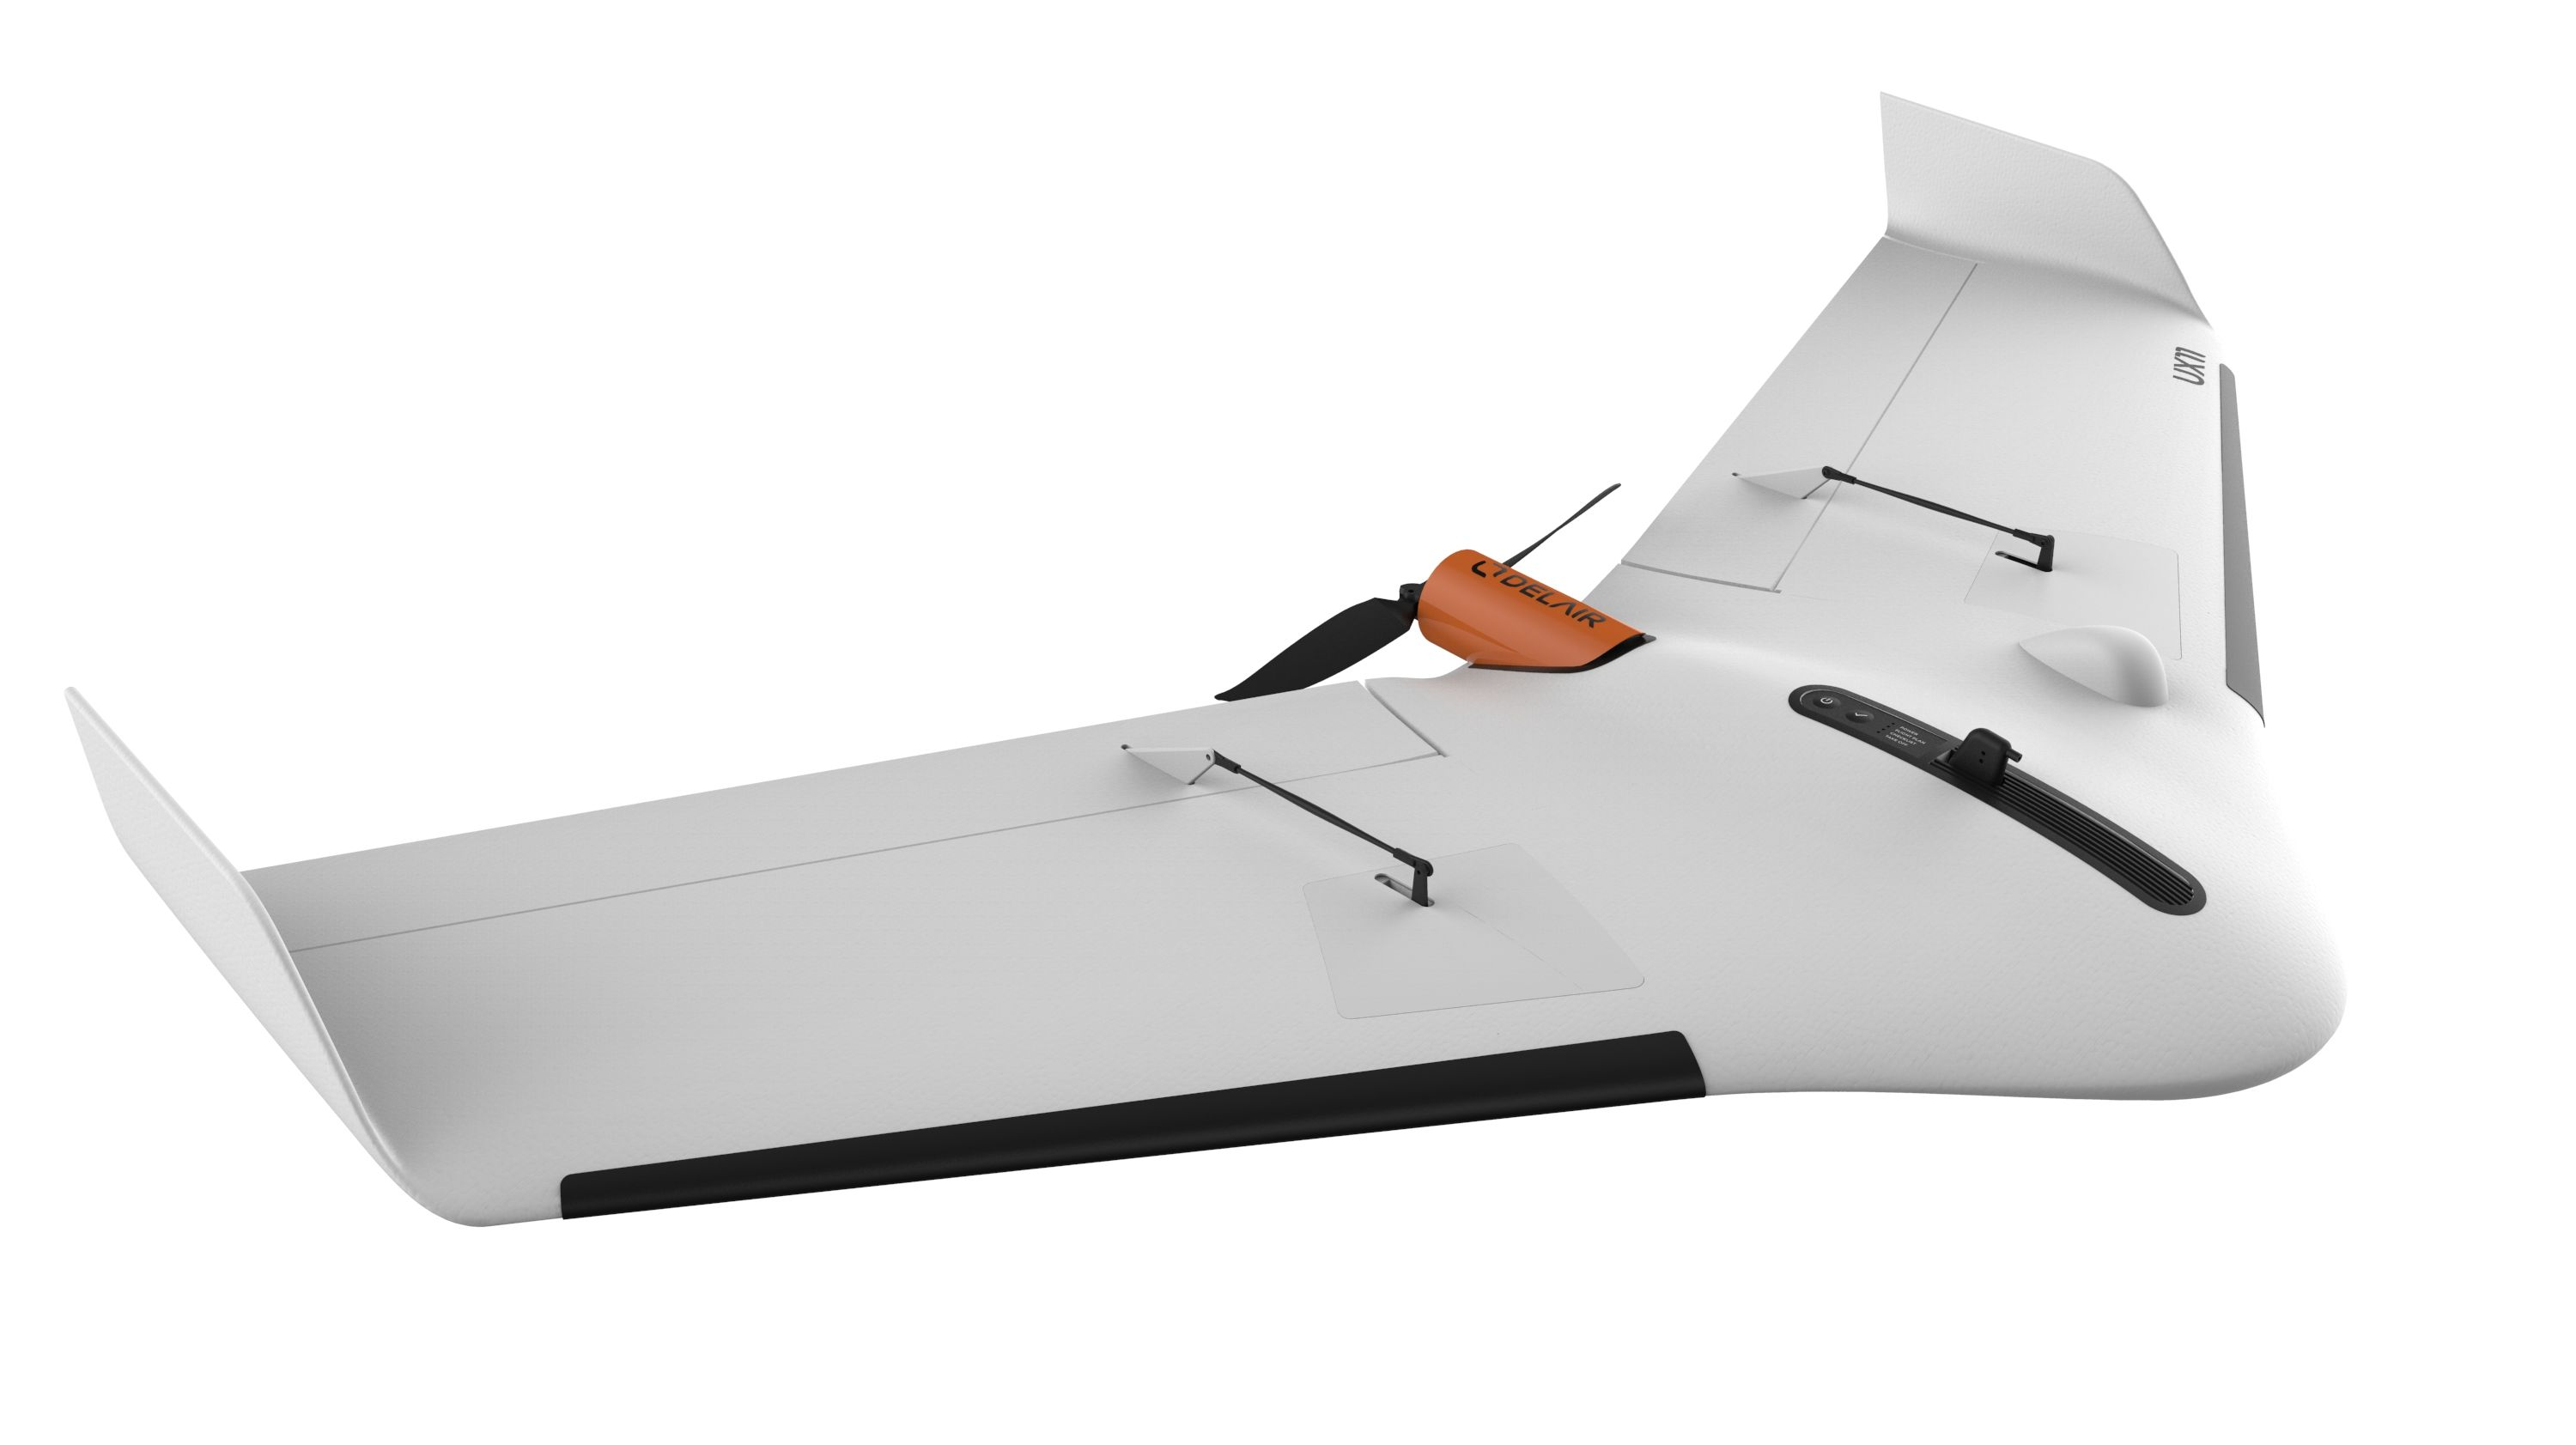
\includegraphics[width=\linewidth]{Images/Introduction/uav-fixed-wing-example.jpg}
      {(a) Fixed-Wing} (\href{https://delair.aero/portfolio/surveying-and-mapping/}{URL})
    \end{minipage}%
    % -----------------
    \begin{minipage}{.5\textwidth}
      \centering
      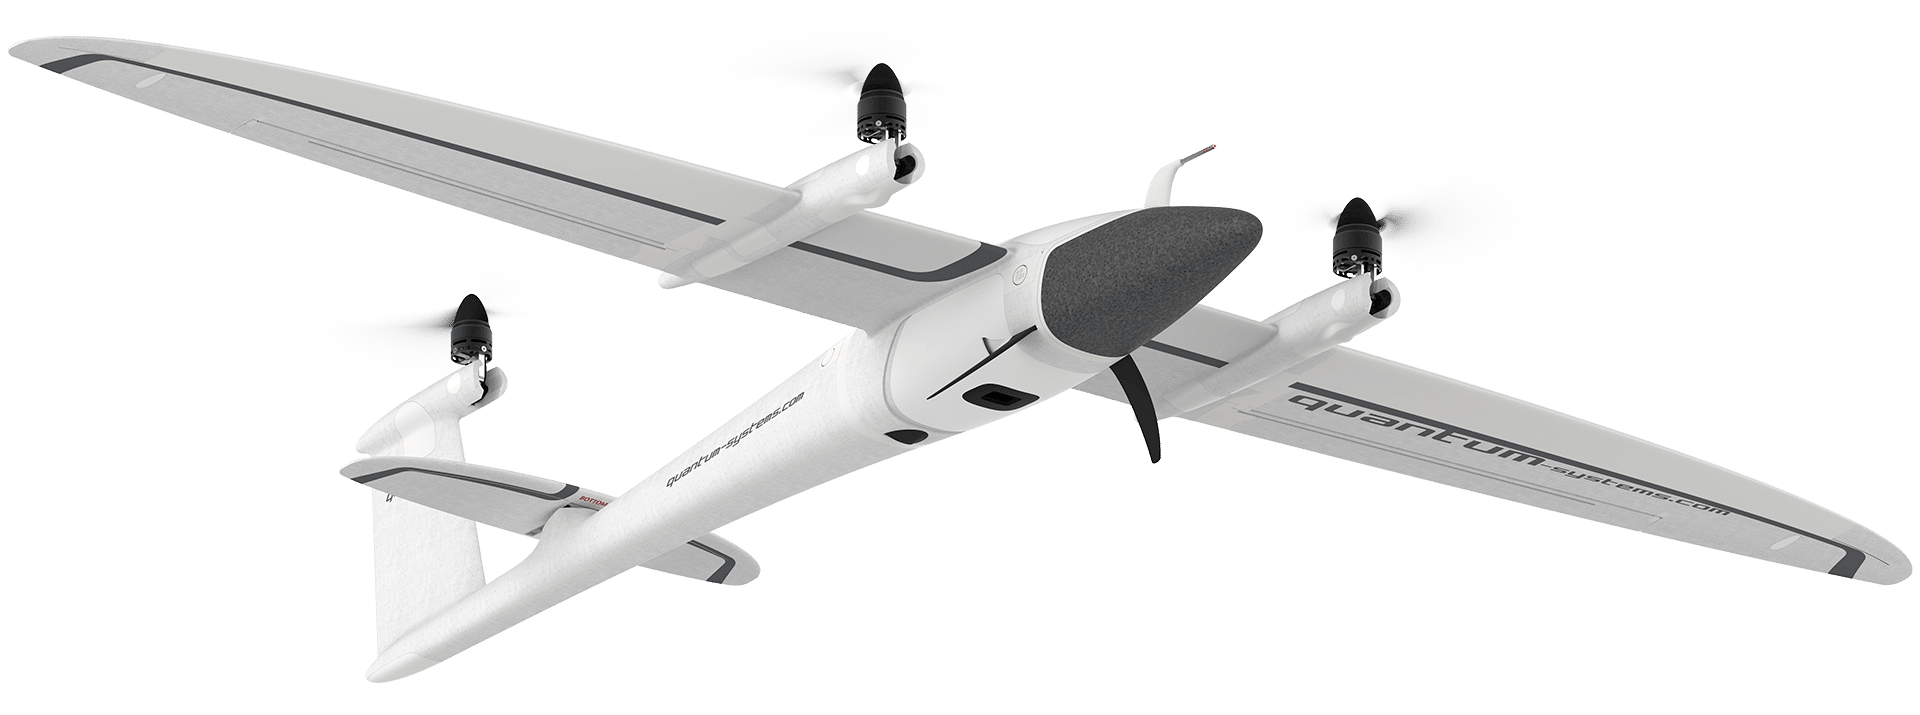
\includegraphics[width=\linewidth]{Images/Introduction/uav-fixed-wing-hybrid-example.png}
      {(b) Fixed-Wing Hybrid} (\href{https://www.quantum-systems.com/project/trinity-f90/}{URL})
    \end{minipage}
    % -----------------
    \begin{minipage}{.5\textwidth}
        \centering
        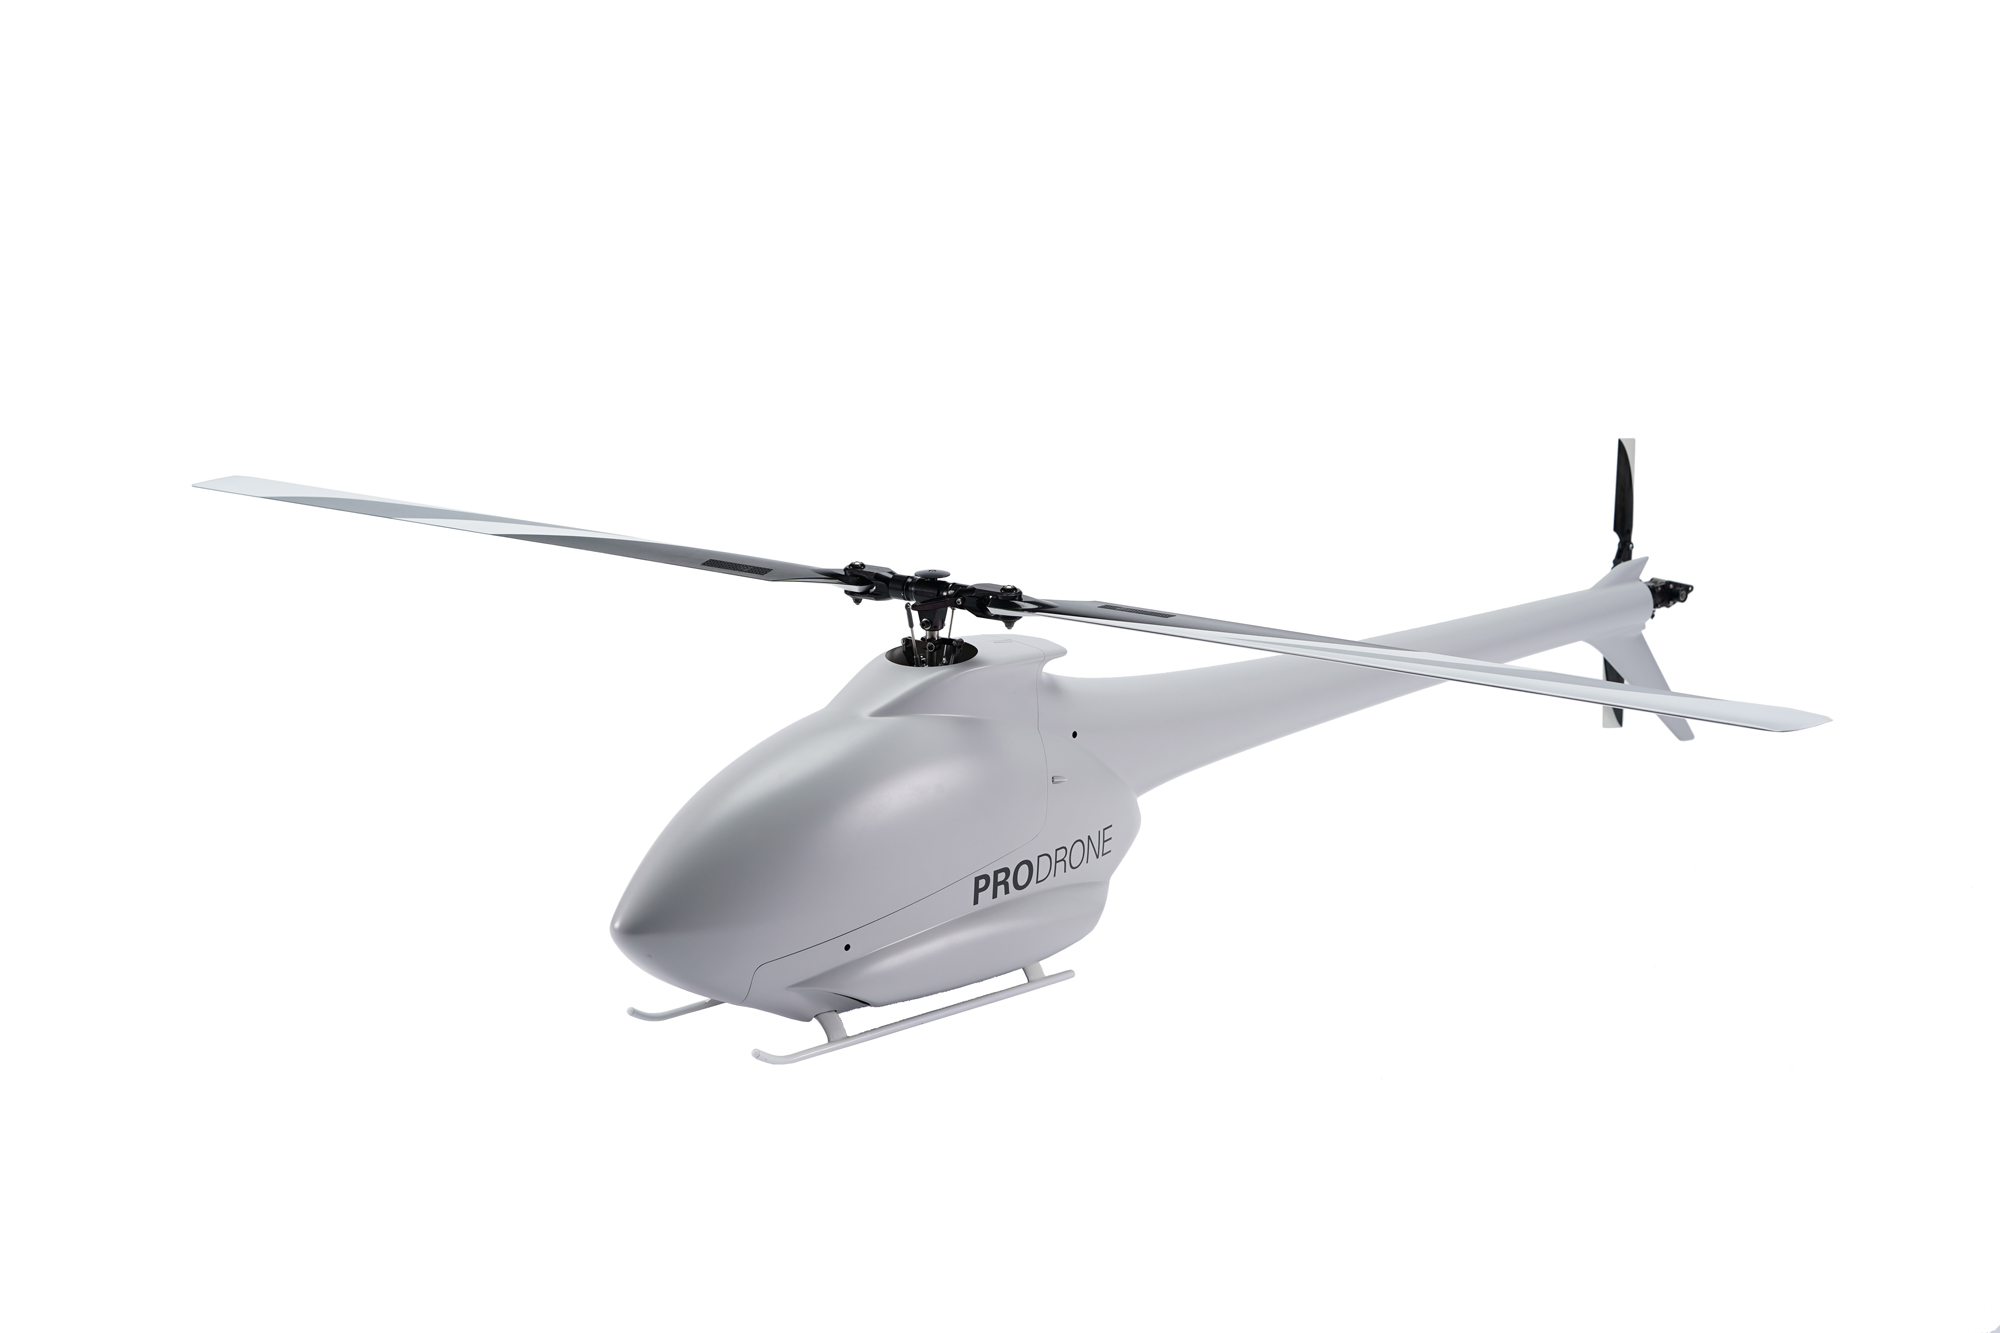
\includegraphics[width=\linewidth]{Images/Introduction/uav-single-rotor-example.jpg}
        {(c) Single Rotor} (\href{https://www.prodrone.com/release-en/2874/}{URL})
      \end{minipage}%
      % -----------------
      \begin{minipage}{.5\textwidth}
        \centering
        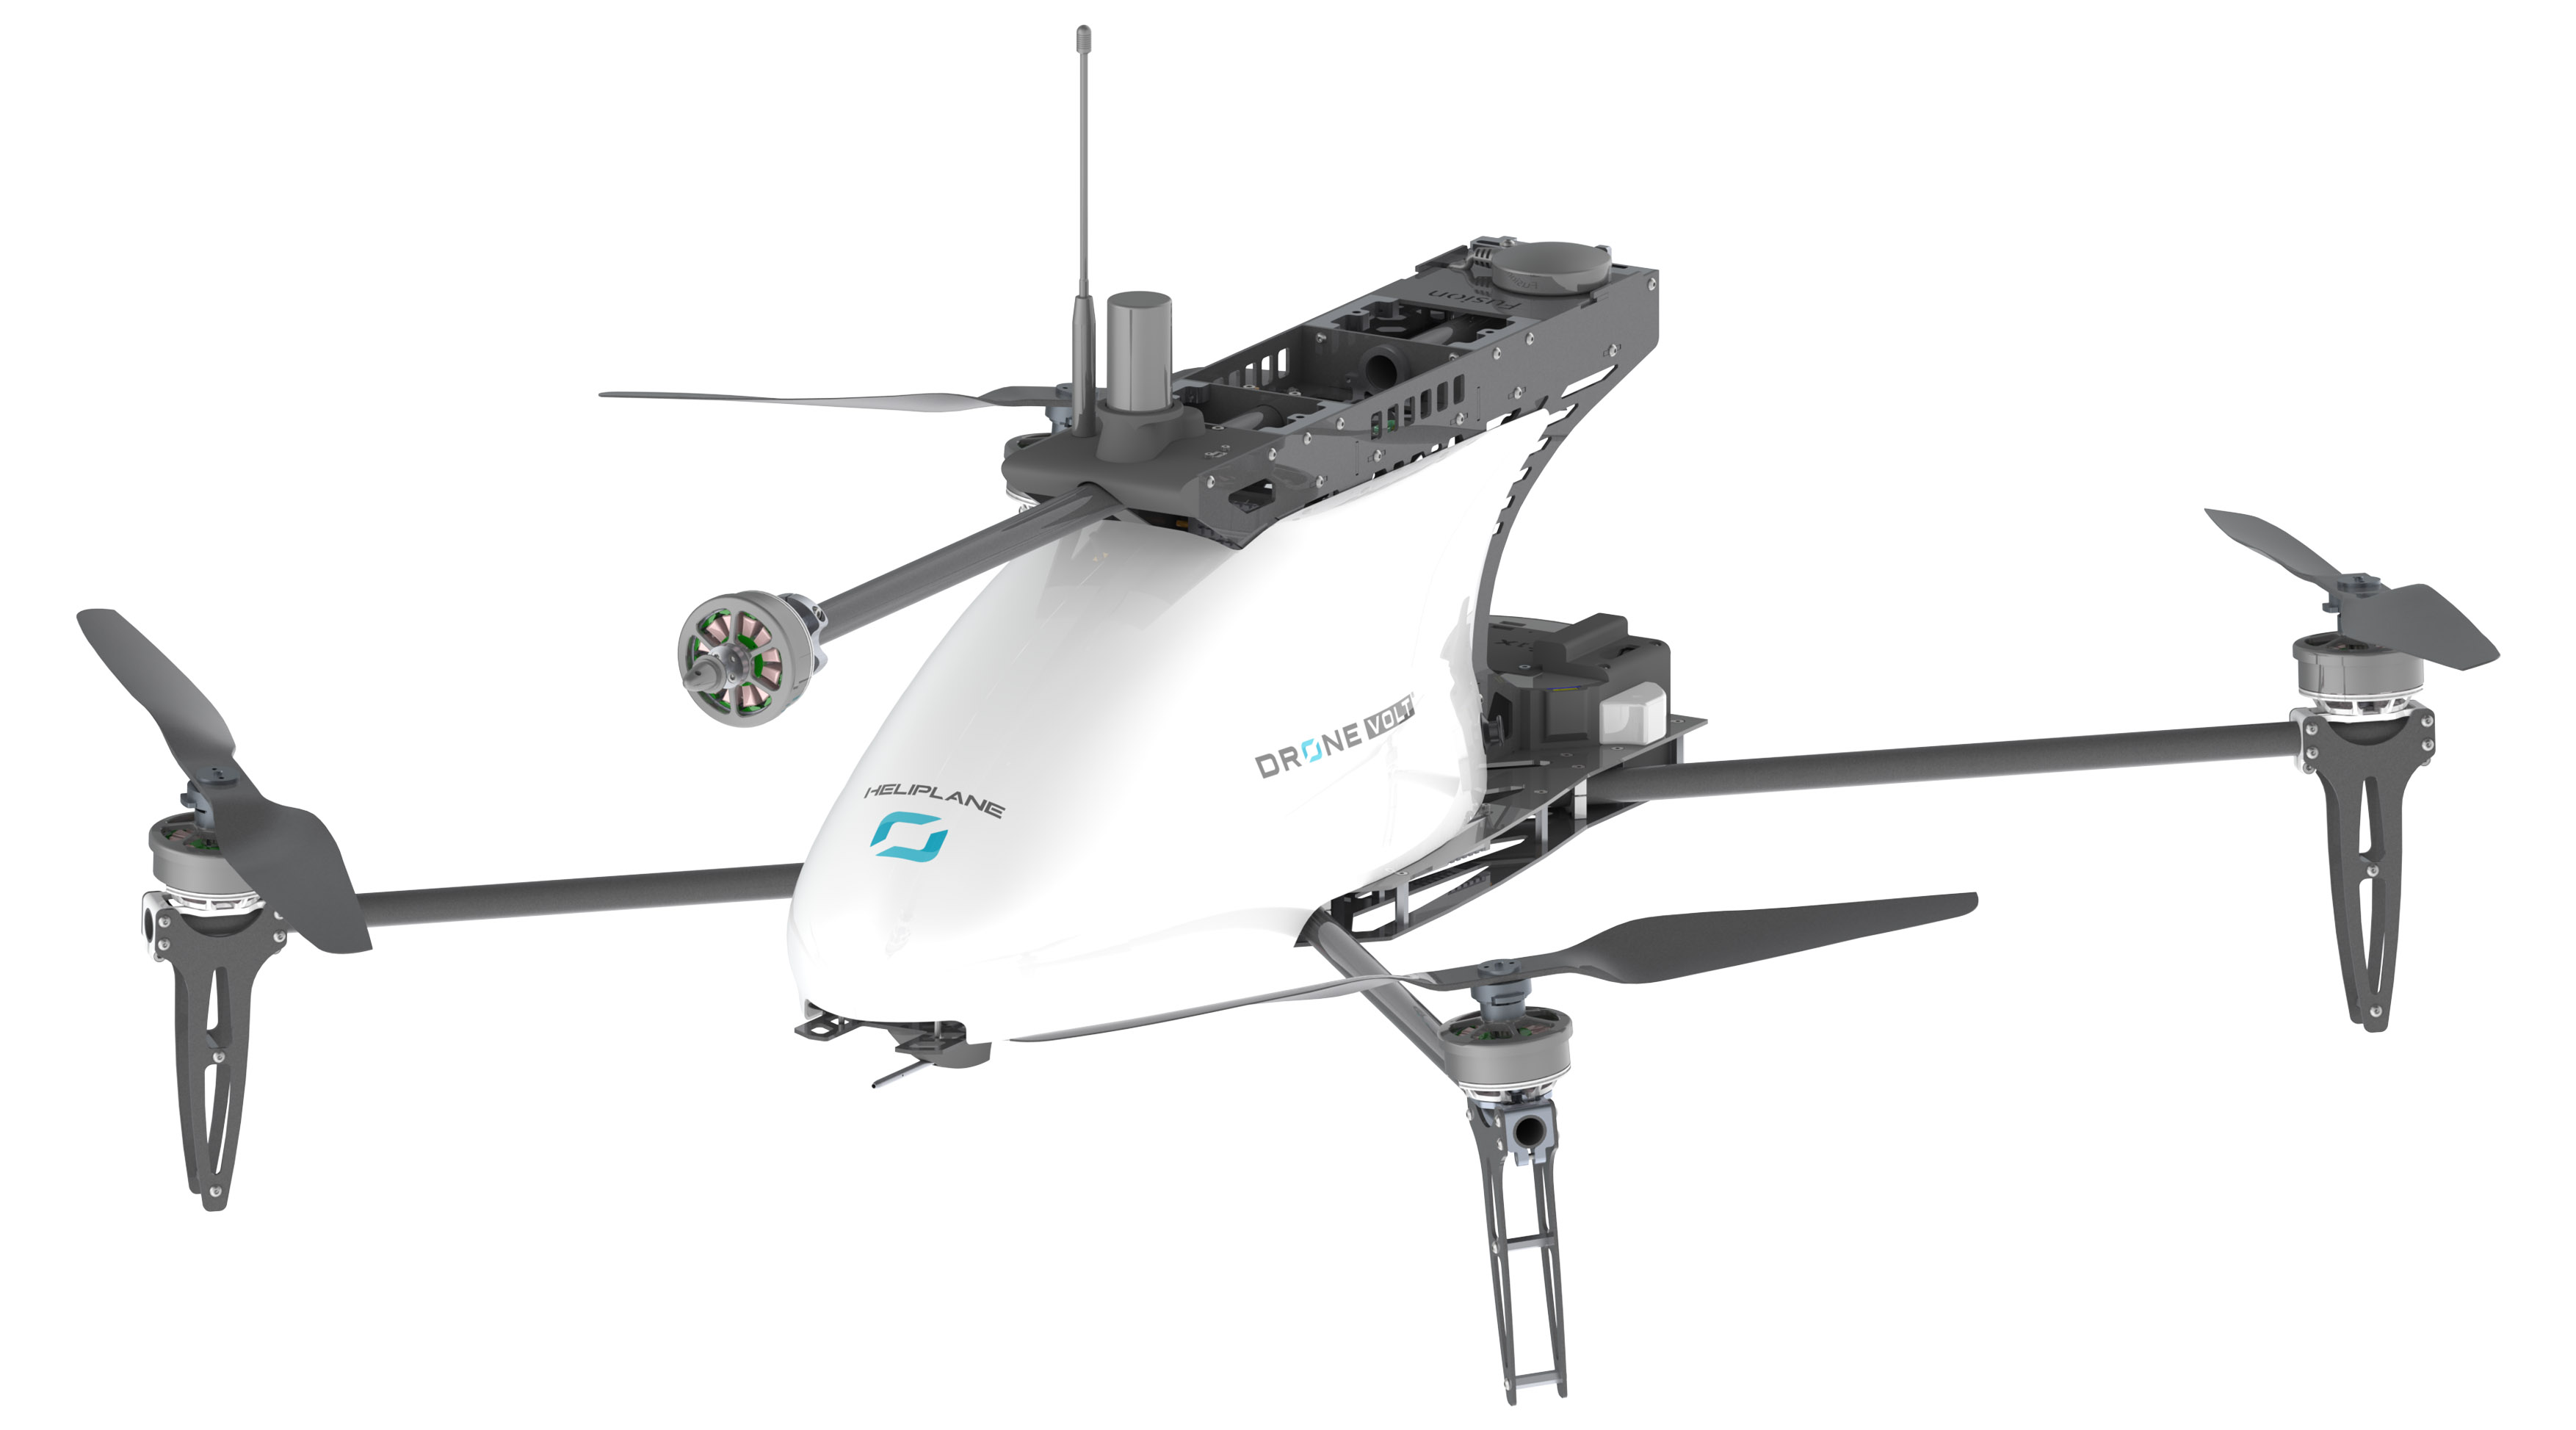
\includegraphics[width=\linewidth]{Images/Introduction/uav-multirotor-example.jpg}
        {(d) Multirotor} (\href{https://metatronus.com/heliplane/}{URL})
      \end{minipage}
      % -----------------
    \hfill \break
    \decoRule
    \caption[UAV Examples]{\hyperref[abbr:UAV]{UAV} Examples}
    \label{fig:UAV-samples}
\end{figure}

Τυπικά τα Fixed-Wing drones είναι αρκετά ακριβά, χρειάζονται εξειδικευμένους χει\-ριστές για να
λειτουργήσουν, όπως επιπλέον και περισσότερο χώρο για την απογείωση και την προσγείωση. Είναι 
ιδανικά για εφαρμογές που χρειάζεται να καλύψουμε μεγάλες περιοχές και συχνά έχουν αυτονομία 
τουλάχιστον μερικών ωρών. Για αυτούς τους λόγους χρησιμοποιούνται κυρίως από κυβερνήσεις,
στρατιωτικές μονάδες ή επιχειρήσεις για την γρήγορη επίβλεψη μεγάλων εκτάσεων \cite{fixed-wing}.  

Τα Fixed-Wing Hybrid προσπαθούν να λύσουν τα μειονεκτήματα που έχουν τα Fixed-Wing drones, την μη ικανότητα 
δηλαδή για  Vertically Hover, Take-off, and Land (\hyperref[abbr:VTOL]{VTOL}) όμως είναι ακόμα σε αρχικά στάδια
\cite{application-areas|swarm-types|uavs-classification|sensor's-used|swarms-problems|public-awareness}.

Τα Single Rotor είναι επίσης αρκετά ακριβά, πολύπλοκα μηχανολογικά μηχανήμα- τα, που δέχονται πολλούς κραδασμούς, 
απαιτούν εξειδικευμένους χειριστές όμως μπορούν να μεταφέρουν αρκετά βαριά payloads, θετικό στην χρήση τους ότι 
μπορούν να πραγματοποιήσουν \hyperref[abbr:VTOL]{VTOL} \cite{application-areas|swarm-types|uavs-classification|sensor's-used|swarms-problems|public-awareness}.

Τα Multirotor είναι ίσως τα πιο ευρέως διαδεδομένα. Καθώς είναι τα πιο οικονομικά από τα παραπάνω και εύκολο να κατασκευαστούν.
Μπορούν να βρεθούν στο εμπόριο με διάφορο πλήθος από έλικες και είναι το κύριο είδος που χρησιμοποιείται από ερασιτέχνες
ή χομπίστες για λόγους αναψυχής \cite{application-areas|swarm-types|uavs-classification|sensor's-used|swarms-problems|public-awareness}.

Στο \emph{Figure} \ref{fig:UAV-samples} δίνονται κάποια ενδεικτικά παραδείγματα \hyperref[abbr:UAV]{UAVs} με βάση την κατηγοριοποίηση
του \emph{Table} \ref{tab:drone-determined-by-their-structure}.
Φυσικά αυτή η κατηγοριοποίηση δεν περιλαμβάνει όλα τα είδη drone, είναι όμως ικανοποιητική για να γίνουν
ξεκάθαρες δύο βασικές ιδέες. Αρχικά ανάλογα με την εφαρμογή που μας ενδιαφέρει, θα πρέπει να επιλέξουμε
την χρήση του πλέον κατάλληλου τύπου drone. Όπως επίσης με βάση την επιλογή του συγκεκριμένου τύπου -
αυτόματα έχουμε να διαχειριστούμε τα πλεονεκτήματα ή τα μειονεκτήματα που έχει.

Σε περίπτωση που μας ενδιαφέρει, οι συγγραφείς του \cite{drone-classification} παρουσιάζουν 
με εκτενέ- στερο τρόπο, διάφορες κατηγοριοποιήσεις
και είδη drone τα οποία δεν εμπίπτουν στα πλαίσια αυτής της διπλωματικής και κυμαίνονται 
από smart dust, bio-drones, hybrid drones και άλλα πολλά.

\subsection{Characteristics} \label{sec:Chapter1-1-2}

Σε όποια από τις κατηγορίες και αν αντιστοιχεί ένα drone
από την στιγμή που είναι ένα ιπτάμενο αντικείμενο, θα πρέπει να έχει την δυνατότητα να κινείται -
φυσικά - στον αέρα. Στο \emph{Figure} \ref{fig:UAV-principal-axes} παρουσιάζονται στους 3 άξονες, τα 6
Degrees of Freedom (\hyperref[abbr:DoF]{DoF}) - τόσο \emph{Transitional} όσο και \emph{Rotational} - ενός \hyperref[abbr:UAV]{UAV} \cite{aircraft-principal-axes} καθώς και το όνομα
που δίνεται στην κίνηση ανάλογα με τον άξονα που πραγματοποιείται.

\begin{figure} [H]
	\centering
	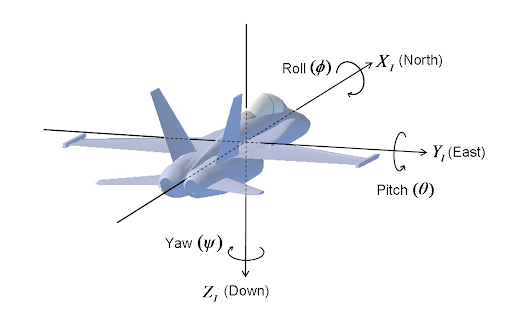
\includegraphics[scale=0.6]{Images/Introduction/aircraft-principal-axes.png}
	\decoRule
	\caption[UAV principal axes]{\hyperref[abbr:UAV]{UAV} principal axes (\href{http://www.chrobotics.com/library/understanding-euler-angles}{URL})}
	\label{fig:UAV-principal-axes}
\end{figure}

Ζούμε σε μία ψηφιακή εποχή, στην οποία ένα από τα πιο σημαντικά κατορθώματα 
είναι η ανάπτυξη των Integrated Circuits (\hyperref[abbr:IC]{IC}s) \& Μicro-electro-mechanical Sy\-stems (\hyperref[abbr:MEMS]{MEMS}) \cite{mems}, 
πράγμα το οποίο έχει βοηθήσει - έξυπνες συσκευές γεμάτες με αισθητήρες να βρίσκονται γύρω μας. 
Τέτοια τεχνολογικά επιτεύγματα όπως τα drones είναι συνεπώς εξοπλισμένα με 
Micro Controller Units (\hyperref[abbr:MCU]{MCU}) \cite{mcu} ή Micro Processor Units (\hyperref[abbr:MPU]{MPU}) \cite{mpu} για 
τον έλεγχο τους, ενώ δεν θα μπορούσαν να μην περιλαμβάνουν πλέον και 
ένα μεγάλο πλήθος και εύρος διαφορετικών τύπων sensors on-board. Με δύο από τους πιο σημαντικούς 
να είναι το Electronic Speed Control (\hyperref[abbr:ESC]{ESC}) \cite{electronic-speed-control}
και το Inertial Measurement Unit (\hyperref[abbr:IMU]{IMU}) \cite{inertial-measurement-unit} - τα οποία 
χρησιμοποιούνται ώστε το drone να μπορεί να διατηρεί μία σταθερή και ελεγχόμενη πτήση \cite{application-areas|swarm-types|uavs-classification|sensor's-used|swarms-problems|public-awareness}.
Εκτός από αυτούς βέβαια, ένα drone μπορεί να διαθέτει Global Positioning System (\hyperref[abbr:GPS]{GPS}), camera 
για λήψη οπτικού υλικού ή ελέγχου μέσω First Person View (\hyperref[abbr:FPV]{FPV}), Obstacle avoidance sensors ή ακόμα και άλλους.
Με κύριο περιορισμό\udot τα αισθητήρια όργανα να βρίσκονται στο εύρος βάρος του payload, που μπορεί να μεταφέρει το drone. 

% Συνοψίζοντας το συγκεκριμένο section, drone μπορεί να θεωρηθεί κάθε μη επανδρωμένη ηλεκτρονικά ελεγχόμενη και εναέρια συσκευή, 
% η οποία κινείται στον χώρο, και χρησιμοποιεί τους on-board αισθητήρες που διαθέτει ώστε να φέρει εις πέρας
% τις λειτουργίες για τις οποίες έχει σχεδιαστεί. 
Σε αυτό το section πραγματοποιήθηκε μία πρώτη οριοθέτηση του όρου drone, παρόλα αυτά
δεν αναφέρθηκαν λόγοι ύπαρξης τους, καθώς και εφαρμογές τους.  Η ύπαρξης των swarms είναι ουσιαστικά η 
κάλυψη των αναγκών από των individual drones σε μεγαλύτερη κλίμακα, για αυτό\udot μερικές από τις εφαρμογές των drone - βρίσκονται
στο \emph{Section} \ref{sec:Chapter1-2-2}.


%----------------------------------------------------------------------------------------
%	SECTION 2
%----------------------------------------------------------------------------------------
\section{Motivation} \label{sec:Chapter1-2} 
Ξεκινώντας από τα individual drones, αξίζει να σημειωθεί ότι το Πολυτεχνείο Κρήτης έχει ένα ενεργό
ερευνητικό ιστορικό στον τομέα των αεροχημάτων. Το SenseLab στο οποίο υπεύθυνος καθηγητής είναι ο κύριος
Παρτσινέβελος της Σχολής Μηχανικών Ορυκτών Πόρων να είναι ένα από αυτά -
και μάλιστα με πολλαπλές διακρίσεις  σε διεθνείς διαγωνισμούς \cite{senselab-site} \cite{senselab-demo}. 

%-----------------------------------------------------------------------------------
\subsection{Nature} \label{sec:Chapter1-2-1}
Στην φύση είναι αρκετά συχνή η ύπαρξη έμβιων οργανισμός που κινούνται σε ομάδες, με μερικά από αυτά ως παράδειγμα, τα σμήνη από πουλιά και
έντομα, κοπάδια ψαριών ή και αγέλες ζώων. Σκοπός της συνεργασίας τους είναι κυρίως η προστασία από θηρευτές ή άλλοι σχετικοί με την επιβίωση.
Αρκετές έρευνες έχουν γίνει εμπνευ- σμένες σε αυτό, ακόμα και στον τομέα των fleet of drones
\cite{research-on-drone-swarms-move-like-animals} \cite{research-on-drone-swarms-move-like-animals-like-documentary} \cite{swarm-of-drones}.
  
%-----------------------------------------------------------------------------------
\subsection{Swarms and Applications} \label{sec:Chapter1-2-2}
Από μόνο του ένα {\hyperref[abbr:UAV]{UAV} σε πολλές περιπτώσεις θα μπορέσει να φέρει εις πέραν την αποστολή 
που του έχει ανατεθεί. Πολύ εύκολα όμως μπορούν να δημιουργηθούν ζητήματα αξιοπιστίας, όταν ένα μεμονωμένο drone
χρειάζεται ως παράδειγμα να χα- ρτογραφήσει σε μικρό χρονικό διάστημα ένα άγνωστο και μεγάλης έκτασης περιβάλλον. Όπως επίσης, εάν θα θέλαμε να
διαθέτει πολλαπλούς αισθητήρες για να έχουμε πιο λεπτομερείς δεδομένα σε μία αποστολή, όμως αυτό να είναι αδύνατον διότι 
υπε- ρβαίνουν το δυνατόν payload που μπορεί να μεταφέρει
το drone. Η ακόμα, και για το ενδεχόμενο αποτυχίας της αποστολής, σε κάποιο πιθανό malfunction που θα πραγματοποιηθεί στο ιπτάμενου όχημα.
Μπορούμε να πούμε λοιπόν\udot σε μία abstract σύγκριση με αυτή των ζώων, ότι ωθούμαστε για ανάλογους σκοπούς στην χρήση των swarms ώστε
να ξεπεράσουμε αυτά τα προβλήματα \cite{reason-for-working-together|related-swarm-research}.  

Με τον όρο swarm συχνά αναφερόμαστε στην μεθοδολογία που ακολουθούμε ώστε να συντονίζουμε πολλαπλές 
ανεξάρτητες ρομποτικές οντότητες να συμπεριφέρονται συνεργατικά ως ένα ενιαίο σύστημα \cite{what-is-swarm-robotics}.
Με τον όρο συνεργατικά, αυτό σημαίνει είτε να μπορούν να κινηθούν ως ομάδα \cite{moving-models-for-robotic-swarms}
\cite{swarm-formation-translation-rotation-attack-demo} \cite{lab-demo-of-formations-in-3d-movement-with-obstacles},
είτε να επικοινωνούν ώστε γνώση πληροφορίας την οποία έχει συλλέξει ένα από αυτά να μεταδίδεται
και στα υπόλοιπα (π.χ. σε περίπτωση που θέλουμε να κάνουμε 3D reconstruction μίας περιοχής ή γνώση της θέσης από 
την οποία λαμβάνεται - με χρήση της κάμερας - υλικό είναι σημαντική για την δημιουργία του ψηφιακού μοντέλου 
\cite{localization-importance-for-3d-scene-reconstruction}). 

Σήμερα τα drones καθώς και τα fleet of drones χρησιμοποιούνται σε ένα μεγάλος εύρος εφαρμογών.
Έχει γίνει αναφορά είδη από την αρχή του chapter ότι χρησιμοποιούνται για λόγους αναψυχής,
με μερικά παραδείγματα, την διεκπεραίωση shows \cite{intel's-shows-around-the-world-and-2018-drones-record}
\cite{ford's-100-drone-show} \cite{swarm-magic-show} και την καταγραφή οπτικού υλικού για δημιουργία 
ταινιών \cite{drones-for-filmmaking}. Άλλες πιο ζωτικής σημασίας χρήσεις τους, είναι σχετικές με 
environment mapping \cite{drones-enviroment-mapping}, police surveillance \cite{drones-police}, natural disaster inspection 
\cite{drones-natural-disaster},  Search \& Rescue (\hyperref[abbr:SR]{S\&R}) \cite{drones-for-search-and-rescue}, 
light cargo transportation \cite{drones-delivery} και πολλές άλλες. Ακόμα και στρατιωτικές επιχειρήσεις 
χρησιμοποιούν drones. Συνήθως σε αυτές τις περιπτώσεις αναφερόμαστε στην χρήση Unmanned Combat Aerial Vehicle (\hyperref[abbr:UCAV]{UCAV}) 
\cite{UCAVs} \cite{military-robots-samples-and-photos} και πολλές από τις εφα\-ρμογές στο συγκεκριμένο
τομέα έχουν να κάνουν με Intelligence Surveillance, and Reconnaissance (\hyperref[abbr:ISR]{ISR})
\cite{drones-isr}.

Για περισσότερες εφαρμογές των drones/swarms \cite{list-of-uav-applications} ή λεπτομέρειες σχετικά με αυτές, μπορούμε να ανατρέξουμε στην υφιστάμενη βιβλιογραφία 
\cite{application-senarios|related-work|the-platform-they-used|communication-infrastructure-and-problems}
\cite{some-applications} \cite{swarm-friendly-communications|brain-sensor-drones|different-swarm-applications|}.

%----------------------------------------------------------------------------------------
%	SECTION 3
%----------------------------------------------------------------------------------------
\section{Scientific Goals and Contributions} \label{sec:Chapter1-3} 
Όπως μπορεί να γίνει εύκολα αντιληπτό η γνώση της σχετικής θέσης ενός {\hyperref[abbr:UAV]{UAV} σε σχέση με τα υπόλοιπα του σμήνους, 
είναι αρκετά σημαντική για ένα πολύ μεγάλο πλήθος εφαρμογών.
Σκοπός της συγκεκριμένης διπλωματικής εργασίας, είναι να γίνει η απαραίτητη ερευνητική
αναζήτηση, ώστε να επιτευχθεί ο σχεδιασμός καθώς και η υλοποίηση ενός ενσωματωμένου συστήματος - το 
οποίο να είναι σε θέση με όσο το δυνατόν πιο οικονομικό τρόπο - να υπολογίζει την θέση των μεμονωμένων
αεροχημάτων όταν αυτά πετούν σε σχηματισμό.  

%----------------------------------------------------------------------------------------
%	SECTION 4
%----------------------------------------------------------------------------------------
\section{Thesis Outline} \label{sec:Chapter1-4} 

    \begin{itemize}
        \item \textbf{Chapter \ref{chap:Chapter2} - {\hypersetup{hidelinks}\nameref{chap:Chapter2}}:} 
          Σε αυτό το κεφάλαιο παρουσιάζεται το απαραίτητο μαθηματικό υπόβαθρο, καθώς και βασικές μεθοδολογίες εύρεσης τοποθεσία, 
          που προέρχονται από τον τομέα των  Wireless Sensor Networks (\hyperref[abbr:WSN]{WSN}).
        \item \textbf{Chapter \ref{chap:Chapter3} - {\hypersetup{hidelinks}\nameref{chap:Chapter3}}:}
        Στην συγκεκριμένη ενότητα γίνεται μία συ\-νο\-πτική αναφορά σε τεχνικές που χρησιμοποιούνται ήδη, σύμφωνα με την βιβλιο\-γραφία,
        για την εύρεσης θέσης μέσα στα swarms.
        \item \textbf{Chapter \ref{chap:Chapter4} - {\hypersetup{hidelinks}\nameref{chap:Chapter4}}:}
        Σε αυτό το σημείο παρουσιάζεται η διαδικασία σχεδιασμού του ενσωματωμένου συστήματος που σχετίζεται αυτή η διπλωματική.
        % \item \textbf{Chapter \ref{chap:Chapter5} - {\hypersetup{hidelinks}\nameref{chap:Chapter5}}:}       %Maybe rename chapter's name
        % TODO:
        \item \textbf{Chapter \ref{chap:Chapter6} - {\hypersetup{hidelinks}\nameref{chap:Chapter6}}:}
        Στο παρόν κεφάλαιο παρουσιάζονται οι απαραίτητοι έλεγχοι που έγιναν για την επαλήθευση της ορθής λειτουργίας του συστήματος.
        \item \textbf{Chapter \ref{chap:Chapter7} - {\hypersetup{hidelinks}\nameref{chap:Chapter7}}:} 
        Στο συγκεκριμένο κεφάλαιο παρουσιάζονται τα τελικά συμπεράσματα τα οποία βγήκαν από το σύνολο της διπλωματικής - 
        καθώς και κάποιες από τις πιθανές μελλοντικές εξελίξεις της.
    \end{itemize}
   % Introduction
\chapter{Theoretical Background} % Main chapter title
\label{chap:Chapter2} % For referencing the chapter elsewhere, use \ref{Chapter1} 
\epigraph{''Let no one ignorant of geometry enter” }{\textit{Plato}}

O χώρος των \hyperref[abbr:WSN]{WSN} έχει και αυτός τα τελευταία χρόνια υψηλό ερευνητικό ενδιαφέρον.
Θα μπορούσε να πει κανείς - λόγο το ότι αποτελεί ένα πιο γενικό κλάδο - περισσότερο από ότι αυτό των 
drones. Συνεπώς θα μεταφερθούμε σε πρώτο επίπεδο στο πιο γενικό φάσμα, αυτό των \hyperref[abbr:WSN]{WSN} 
για να προσεγγίσουμε το localization problem. 

Όταν μιλάμε για \hyperref[abbr:WSN]{WSN}, αναφερόμαστε σε αυτόνομα ηλεκτρονικά συστήματα, χωρικά διασκορπισμένα σε ένα πεδίο - τα οποία συχνά περιλαμβάνουν
αισθητήρες και επικοινωνούν με τα γειτονικά τους ή σταθμούς βάσης για να μεταφέρουν πληροφορία \cite{wsn-wikipedia} \cite{farooqiazam2016location}.

Το καθένα από αυτά τα ανεξάρτητα συστήματα ονομάζεται \textbf{Node}. Ενώ για το κάθε μεμονωμένο node 
μπορεί να έχουμε στην διάθεση μας location information ή όχι. 
Μία πρώτη σκέψη θα ήταν κάθε node ενός συστήματος αισθητήρων να περιλαμβάνει \hyperref[abbr:GPS]{GPS} ώστε να γνωρίζουμε 
την θέση του. Αυτό μπορεί γρήγορα να καταρριφθεί σαν σκέψη, αν αναλογιστούμε αρχικά ότι το Global Navigation Satellite System (\hyperref[abbr:GNSS]{GNSS})
δεν είναι διαθέσιμο σε κάθε περιβάλλον λειτουργίας (π.χ. εσωτερικούς χώρους), όπως επίσης μπορεί να μην είναι δυνατή η χρήση του σε όλους τους κόμβους
ενός συστήματος, λόγο περιορισμών όπως το κόστος, μέγεθος του node και energy consumption \cite{farooqiazam2016location}.   

\begin{table}[H]
    \caption{Nodes' names definitions}
    \label{tab:nodes-names-definition}
	\centering
	\resizebox{1\textwidth}{!}{
		\begin{tabular}{ll}
			\toprule
			\textbf{Node name} & \textbf{Definition}  \\
			\midrule
				Unknown/Free/Dumb/Non-anchors & Their position is unknown \\
				Beacons/Anchors/Landmarks & Nodes with known location information \\
				Settled & Initial unknown nodes with estimated position \\
			\bottomrule
		\end{tabular}
	}
\end{table}

Στην υπάρχουσα βιβλιογραφία \cite{farooqiazam2016location} \cite{wsn-Localization-systems} \cite{wsn-Localization-techniques} βρίσκουμε ότι
nodes των οποίων η θέση είναι γνωστή ή άμεσα υπολογίσιμη, συχνά ονομάζονται \textbf{Beacons}. Πληροφορία σχετικά με την θέση αυτών
των nodes είναι γνωστή, είτε γιατί έχουν τοποθετηθεί από εμάς σε προκαθορισμένες θέσεις, είτε μέσου ενός εξωτερικού συστήματος
όπως το \hyperref[abbr:GPS]{GPS} \cite{angle-of-arrival}.
Αντίθετα κόμβοι για τους οποίους δεν έχουμε αρχικά πληροφορία της θέσης τους, ονομάζονται \textbf{Non-anchors}.
Άλλος ένας σημαντικός ορισμός, που θα πρέπει να αναφερθεί είναι ότι συχνά ονομάζουμε \textbf{Settle} nodes, 
αυτά τα οποία αρχικά δεν γνωρίζαμε την θέση τους αλλά στην συνέχεια την εκτιμήσαμε.
Στο Table \ref{tab:nodes-names-definition} παρουσιάζονται συνοπτικά τα διάφορα ονόματα που έχουν δοθεί ανά 
καιρούς για το κάθε τύπο node.

Σκοπός ενός localization system είναι, με χρήση της γνώσης που έχουμε για τα beacon nodes να εκτιμήσουμε
την θέση όσο περισσότερων unknown nodes ώστε να τα μετατρέψουμε σε settled nodes και η εκτίμηση της κάθε
θέσης να είναι με όσο το δυνατόν μικρότερο error απόκλισης. 

\begin{figure} [H]
	\centering
	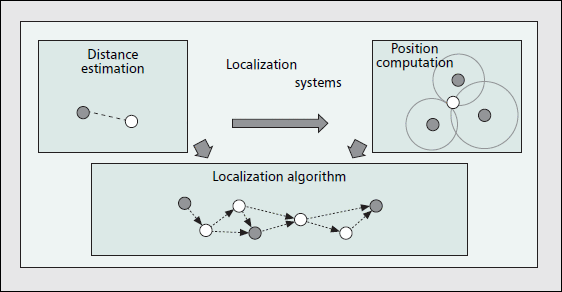
\includegraphics[scale=0.5]{Images/Theoretical-Background/localization-systems-components.png}
	\decoRule
	\caption[Localization System components]{Localization System components based on \cite{wsn-Localization-systems} (\href{https://ieeexplore.ieee.org/document/4407221}{URL})}
	\label{fig:Localization-Systems-components}
\end{figure}

Οι συγγραφείς του \cite{wsn-Localization-systems} επιχειρούν να χωρίσουν ένα localization system, ώστε 
αυτό να αποτελείται από τρία διακριτά components, αυτή τη κατηγοριοποίηση την υιοθετούν κατά την έρευνα τους και οι ερευνητές του \cite{localization-systems-components}. Πρώτο μπορεί να θεωρηθεί αυτό του \textbf{Distance/Angle Estimation}, 
που σκοπό έχει να υπολογίσει την απόσταση ή γωνία που έχουν δύο nodes του συστήματος μεταξύ τους.
Η πληροφορία που θα παραχθεί από αυτό το component θα χρησιμοποιηθεί στα άλλα μέρη του συστήματος.
Στην συνέχεια υπάρχει το \textbf{Position Computation}, δουλειά του οποίου είναι να υπολογίσει την θέση ενός
node με βάση την γνώση που έχουμε για τα beacons και την πληροφορία που λάβαμε από το πρώτο component.
Ενώ τέλος είναι το κύριο μέρος του συστήματος, με όνομα \textbf{Localization Algorithm} και ουσιαστικά είναι
ο προκαθορισμένος τρόπος που θα ακολουθηθεί για να υπολογιστεί η θέση των unknown nodes με βάση όλες τις 
πληροφορίες που έχουμε.
Στο Figure \ref{fig:Localization-Systems-components} δίνεται η απεικόνιση που έδωσαν οι συγγραφείς του 
\cite{wsn-Localization-systems} για να εξηγήσουν το παραπάνω. Ενώ στο Figure \ref{fig:Localization-system}
έχει γίνει μία προσπάθεια να κατηγοριοποιηθούν τα κομμάτια καθώς και τεχνικές των Localization Systems,
με βάση τα \cite{farooqiazam2016location} \cite{wsn-Localization-systems} \cite{wsn-Localization-techniques}
και αναλύονται στην συνέχεια του κεφαλαίου.

\begin{figure} [H]
	\tikzset{
		basic/.style  = {draw, text width=2cm, font=\sffamily},
		root/.style   = {basic, thin, align=center, fill=white, text width=5cm},
		level 1/.style = {sibling distance=16em, level distance=5em},
		level-2/.style = {basic, thin, align=center, fill=white, text width=5.5cm},
		level-31/.style = {basic, thin, align=center, fill=white, text width=2cm},
		level-32/.style = {basic, thin, align=center, fill=white, text width=2.8cm},
		level-33/.style = {basic, thin, align=center, fill=white, text width=5cm},
		level-4/.style = {basic, thin, align=center, fill=white, text width=4.5cm},
		level-42/.style = {basic, thin, align=center, fill=white, text width=4.8cm},
		edge from parent/.style={->,solid,black,thick,draw}, 
		edge from parent path={(\tikzparentnode.south) -- (\tikzchildnode.north)},
		>=latex, node distance=1.5cm, edge from parent fork down
	}
	\centering
	\resizebox{1\textwidth}{!}{
		\begin{tikzpicture}[]
			\node[root] {\textbf{Localization Systems}}
				child {node[level-2] (c1) {\textbf{Distance/Angle Estimation}}}
				child {node[level-2] (c2) {\textbf{Position Computation}}}
				child {node[level-2] (c3) {\textbf{Localization Algorithm}}};
			
			% -----------------------------------------------------------------------------
			% Distance/Angle
			\node [level-31, below of = c1, xshift=-25pt] (c11) {Distance};
				\node [level-4, below of = c11, xshift=50pt] (c111) {Received Signal Strength};
				% \node [level-4, below of = c111] (c112) {Lighthouse approach};
				\node [level-4, below of = c111] (c113) {Propagation time based measurements};
					\node [level-42, below of = c113, xshift=30pt] (c1131) {One-way propagation time};
					\node [level-42, below of = c1131] (c1132) {Roundtrip propagation time};
					\node [level-42, below of = c1132] (c1133) {Time Difference of Arrival};
					\foreach \value in {1,2,3} \draw[->] (c113.197) |- (c113\value.west);
				\foreach \value in {1,3} \draw[->] (c11.195) |- (c11\value.west);

			\node [level-31, below of = c1133, xshift=-80pt] (c12) {Angle};
				\node [level-4, below of = c12, xshift=70pt] (c121) {Receiver Antenna Amplitude response};
				\node [level-4, below of = c121] (c122) {Receiver Antenna Phase response};
				\foreach \value in {1,2} \draw[->] (c12.210) |- (c12\value.west);
			\foreach \value in {1,2}   \draw[->] (c1.188) |- (c1\value.west);
			
			% Position Computation
			\node [level-32, below of = c2, xshift=25pt] (c21) {Trilateration};
			\node [level-32, below of = c21] (c22) {Bounding box};
			\node [level-32, below of = c22] (c23) {Triangulation};
			\node [level-32, below of = c23] (c24) {Multilateration};
			\node [level-32, below of = c24] (c25) {Probabilistic approaches};
			\node [level-32, below of = c25] (c26) {Central position};
			\foreach \value in {1,...,6} \draw[->] (c2.196) |- (c2\value.west);

			% Localization Algorithm
			\node [level-33, below of = c3, xshift=10pt] (c31) {Range-based/Range-free};
			\node [level-33, below of = c31] (c32) {Distributed/Centralized \\ Position Computation};
			\node [level-33, below of = c32] (c33) {Relative/Absolute Positioning};
			\node [level-33, below of = c33] (c34) {Indoor/Outdoor scenarios};
			\node [level-33, below of = c34] (c35) {One-hop/Multihop};
			\node [level-33, below of = c35] (c36) {With/Without Infrastructure};
			\foreach \value in {1,...,6} \draw[->] (c3.187) |- (c3\value.west);
		\end{tikzpicture}
	}
	\decoRule
	\caption[Localization System overview]{Localization System overview}
	\label{fig:Localization-system}
\end{figure}

Με βάση τον παραπάνω διαχωρισμό των Localization Systems σε τρία διακριτά μέρη, μπορούμε να καταλάβουμε
ότι η απόκλιση της εκτίμησης του συνολικού συστήματος, εξαρτάται από τα σφάλματα  του κάθε μεμονωμένου μέρους.

%----------------------------------------------------------------------------------------
%	SECTION 1
%----------------------------------------------------------------------------------------
\section{Distance/Angle Estimation} \label{sec:Chapter2-1} 

\subsection{Distance}\label{sec:Chapter2-1-1}

Θα ξεκινήσουμε με μία σύντομη ανάλυση των τεχνικών εκτίμησης της απόστασης μεταξύ δύο nodes
που χρησιμοποιούνται ήδη. 

%----------------------------------------------------------------------
\subsubsection{Received Signal Strength}
Η πρώτη τεχνική η οποία έχει χρησιμοποιηθεί για τον υπολογισμό απόστασης στα 
\hyperref[abbr:WSN]{WSN}, είναι αυτή με όνομα Received Signal Strength Indicator
(\hyperref[abbr:RSSI]{RSSI}) και έχει ως αρχή την χρήση της έντασης της ισχύς ενός 
σήματος που λαμβάνουμε στον δέκτη, ως τρόπο υπολογισμού της απόστασης
του πομπό από αυτόν. Path loss ή path attenuation \cite{wikipedia-Path_loss} ονομάζεται η μείωση της ισχύς
ενός σήματος καθώς αυτό διαδίδεται.
Στον ελεύθερο χώρο η λαμβανόμενη ισχύς $P_r(d)$ που ανιχνεύει ο πομπός
μπορεί να περιγραφτεί από το μοντέλο του Free Space Path Loss (\hyperref[abbr:FSPL]{FSPL}) \cite{wikipedia-fspl}, το οποίο προκύπτει
μέσω της Friis transmission equation \cite{wsn-Localization-techniques} \cite{rssi-wlan} \cite{wikipedia-friis-equation} - σχέση (\ref{eq:signal-strength}).

\begin{align}
	P_r(d)=\frac{P_tG_tG_r\lambda^2}{(4\pi)^2d^2} \label{eq:signal-strength}
\end{align}

Όπου $P_t$ είναι η ισχύς που στέλνει ο πομπός, $G_t$ είναι το gain της κεραίας του
πομπού, $G_r$ το gain της κεραίας του δέκτη, λ είναι το μήκος κύματος του σήματος
το οποίο μεταδίδουμε και d η απόσταση του πομπού από τον δέκτη. Αν θεωρήσουμε ότι 
τα $G_t$, $G_r$ και λ είναι μη μεταβλητές τιμές - με $C_f = \frac{G_tG_r\lambda^2}{(4\pi)^2}$ - τότε μπορούμε να καταλήξουμε
στην (\ref{eq:signal-strength-simple}) \cite{rssi-simple-formula}.

\begin{align}
	P_r(d)=C_f\frac{P_t}{d^2} \label{eq:signal-strength-simple}
\end{align}

Αυτό που μπορούμε να δούμε από την παραπάνω σχέση είναι ότι, ιδανικά στον ελεύθερο 
χώρο σε Line of Sight (\hyperref[abbr:LoS]{LoS}) μετάδοση -
η ισχύς του σήματος που λαμβάνει ο πομπός εξαρτάται από το αντίστροφο τετράγωνο της
απόστασης των δύο nodes. Η σχέση (\ref{eq:signal-strength-simple}) συχνά αναφέρεται σε watt, 
όμως όταν μιλάμε για transmitting power αντί για την χρήση των watt, είναι αρκετά βολική
η χρήση του dBm \cite{wikipedia-dBm}. Για αυτό τον λόγω παρακάτω παραπείθονται τα conversion
equations, από το ένα στο άλλο \cite{rssi-wlan} \cite{wikipedia-dBm}. 

\begin{align}
	\left\{
		\begin{array}{ll}
			P[dBm]= 10\cdot log_{10}\left(\frac{P[mW]}{1[mW]}\right) \\[10pt]
			\quad \quad P[mW] = 10^\frac{(P[dBm])}{10}
		\end{array}
	\right.
\end{align}

Ενώ το Figure \ref{fig:Ideal-RSSI-over-distance} περιγράφει σχηματικά το ιδανικό μοντέλο της εξάρτηση της ισχύς με την αύξηση
της απόστασης όταν χρησιμοποιούμε στον δέκτη μέτρηση σε dΒm. 

%-------------------------------------------

\begin{figure} [H]
	\centering
	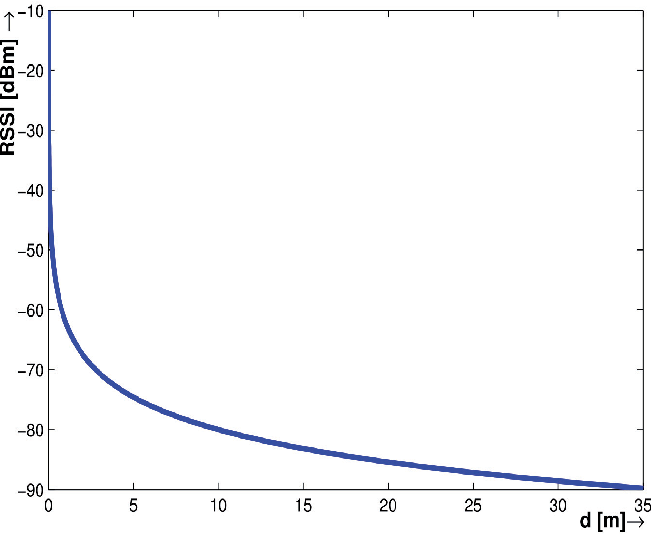
\includegraphics[scale=0.32]{Images/Theoretical-Background/Ideal-RSSI-over-distance.png}
	\decoRule
	\caption[Ideal RSSI over distance]{Ideal RSSI over distance based on \cite{ideal-rssi-model}}
	\label{fig:Ideal-RSSI-over-distance}
\end{figure}

Αν λοιπόν, μετράμε την ισχύ με την οποία λαμβάνουμε ένα σήμα, μπορούμε να είμαστε σε θέση να υπολογίσουμε την απόσταση που βρίσκεται
ο πομπός από εμάς.
Αυτή η μέθοδος παρόλο που είναι αρκετά δημοφιλής και οικονομική για τον υπολογισμό της απόστασης
- λόγω του ότι δεν απαιτεί επιπλέον αισθητήρες - σε πραγματικές 
συνθήκες αντιμετωπίζει αρκετά προβλήματα, καθώς οι μετρήσεις μπορούν να επηρεαστούν από θόρυβο,
ανακλάσεις του σήματος, διαθλάσεις, δυναμικά περιβάλλοντα ή εμπόδια σε αυτά, Non-Line of Sight (\hyperref[abbr:NLoS]{NLoS}) μετάδοση, 
ή ακόμα και errors στο hardware 
\cite{wsn-Localization-systems} \cite{ideal-rssi-model}.
Σε ένα βαθμό μπορεί να βελτιωθεί η απόδοση με στατικό ή δυναμικό calibration του συστήματος 
όμως μέχρι τώρα δεν χρησιμοποιείται για εκτίμηση απόστασης σε εφαρμογές όπου nodes έχουν μεγάλη
απόσταση μεταξύ τους ή μας ενδιαφέρει να έχουμε μεγάλη ακρίβεια προσέγγισης της απόστασης \cite{ideal-rssi-model}.

%----------------------------------------------------------------------
\subsubsection{Propagation Time}
Σε αυτήν την κατηγορία εκτίμησης απόστασης μεταξύ nodes - η οποία βασίζεται σε χρονικές μετρήσεις της διάδοσης του σήματος Time of Flight (\hyperref[abbr:ToF]{ToF})
- κατά κύριο λόγο χρησιμοποιούνται δύο βασικές τεχνικές, η Time of Arrival (\hyperref[abbr:ToA]{ToA}) και η Time 
Difference of Arrival (\hyperref[abbr:TDoA]{TDoA}) \cite{wsn-Localization-systems}. 

\begin{figure} [H]
    \centering
    % -----------------
    \begin{minipage}{.5\textwidth}
      \centering
      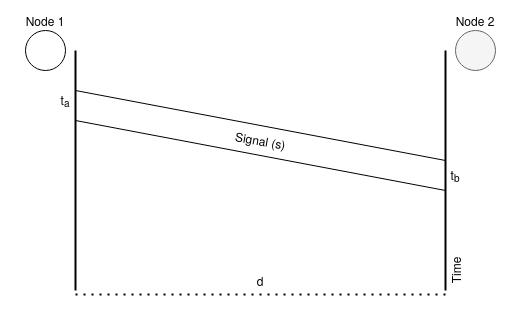
\includegraphics[width=\linewidth]{../Photos/toa-oneway.png}
      {(a) One-way}
    \end{minipage}%
    % -----------------
    \begin{minipage}{.5\textwidth}
      \centering
      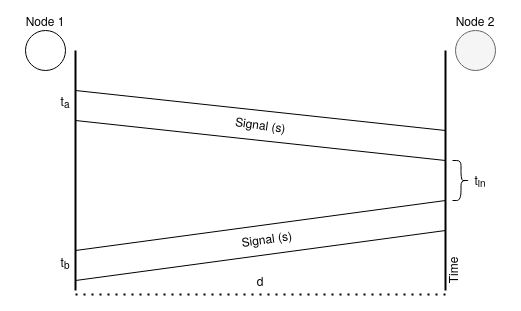
\includegraphics[width=\linewidth]{../Photos/toa-roundtrip.png}
      {(b) Roundtrip}
    \end{minipage}
    \hfill \break
    \decoRule
    \caption[Time of Arrival cases]{Time of Arrival cases}
    \label{fig:Time-of-Arrival-cases}
\end{figure}

Θα ξεκινήσουμε με μία σύντομη περιγραφή της \hyperref[abbr:ToA]{ToA}. Από την κινηματική γνωρίζουμε την 
σχέση (\ref{eq:speed}), η οποία συσχετίζει την ταχύτητα κίνησης ενός σώματος V ως το πηλίκο της μεταβολής
της θέσης $\mathrm{d}s$ - που έκανε το σώμα, προς τον χρόνο $\mathrm{d}t$ που χρειάστηκε για να πραγματοποιηθεί η μεταβολή \cite{Kinematics}.

\begin{align}
	V=&\frac{\mathrm{d}s}{\mathrm{d}t} \label{eq:speed} \\
	d=&s(t_b-t_a) \label{eq:tod-distance}
\end{align}

Αξιοποιώντας την (\ref{eq:speed}) ως αρχή, μπορούμε να καταλήξουμε στην (\ref{eq:tod-distance}) για να εκτιμήσουμε
την απόσταση d που βρίσκονται δύο nodes μεταξύ τους, αν ένα κύμα κινείται με ταχύτητα $s$ και χρειάστηκε 
χρόνο $t$ για να μεταδοθεί από το ένα node στο άλλο. Στο Figure \ref{fig:Time-of-Arrival-cases} (a) απεικονίζεται
σχηματικά αυτό, όπου $t=t_b-t_a$ με $t_b$ η χρονική στιγμή που φτάνει το κύμα στο receiver και $t_a$
η χρονική στιγμή η οποία ξεκινάει από τον transmitter. Σε περίπτωση που μιλάμε για Radio Frequency 
(\hyperref[abbr:RF]{RF}) η ταχύτητα μετάδοσης του κύματος είναι ίση με την ταχύτητα μετάδοσης του φωτός $c_o$, το οποίο 
σε $1μs$ διανύει περίπου 300m.
Με βάση αυτό, μπορούμε εύκολα να καταλάβουμε ότι για να έχουμε ακριβή αποτελέσματα είναι αρκετά σημαντικό
τα clocks των δύο nodes να είναι απόλυτα συγχρονισμένα για να μην έχουμε error απόκλισης, πράγμα που
απαιτεί να κάνουμε το συνολικό σύστημα αρκετά πιο πολύπλοκο σχεδιαστικά 
ώστε η απόκλιση μας να είναι σε ανεκτά σημεία για την εφαρμογή \cite{wsn-Localization-systems} \cite{wsn-Localization-techniques}.

Μπορούμε να το παρακάμψουμε αυτό, με το να γίνει η μέτρηση σε roundtrip μετάδοση, Figure \ref{fig:Time-of-Arrival-cases} (b).
Σε αυτήν την περίπτωση το ένα node στέλνει ένα σήμα, και μόλις το λάβει ένα γειτονικό node, απαντάει πίσω στο πρώτο. 
Με αυτόν τον τρόπο η μέτρηση του χρόνου εκκίνησης $t_a$ και άφιξης $t_b$ του σήματος γίνονται στο ίδιο node - 
άρα δεν χρειάζεται συγχρονισμός, και η πραγματική απόσταση είναι η μισή από αυτή που θα υπολογιστεί. Ο κύριος παράγοντας
σφάλματος σε αυτή την μέθοδο, είναι ο υπολογισμός του χρόνου που χρειάστηκε το δεύτερο node για να διαχειριστεί
το σήμα που έλαβε και να απαντήσει. Αυτό το internal delay $t_{in}$ μπορεί να είναι είτε γνωστό από 
ένα a priori calibration, είτε μπορεί να μετριέται και να στέλνεται μαζί με το σήμα απάντησης - ώστε να αφαιρείται
από τον χρόνο μετάδοσης του κύματος \cite{wsn-Localization-techniques}.
Με αυτά τα δεδομένα η σχέση (\ref{eq:toa-roundtrip}) περιγράφει τον τρόπο υπολογισμού της
απόστασης d μεταξύ των δύο nodes.

\begin{align}
	d=\frac{s(t_b-t_a-t_{in})}{2} \label{eq:toa-roundtrip}
\end{align}


Όσον αφορά την τεχνική \hyperref[abbr:TDoA]{TDoA}, και σε αυτήν την περίπτωση υπάρχουν δύο παραλλαγές της \cite{wsn-Localization-systems} - όπου και οι 
δύο είναι βασισμένες στην αρχή το ότι δεν μας ενδιαφέρει η χρονική στιγμή που ξεκίνησε η αποστολή ενός σήματος, αλλά μόνο
οι χρονική στιγμή που το λάβαμε.

\begin{figure} [H]
    \centering
	% -----------------
    \begin{minipage}{.5\textwidth}
      \centering
      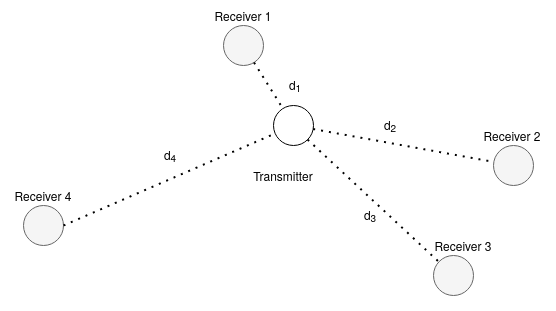
\includegraphics[width=\linewidth]{../Photos/tdoa-multiple.png}
      {(a) Single signal - multiple receivers}
    \end{minipage}%
    % -----------------
    \begin{minipage}{.5\textwidth}
      \centering
      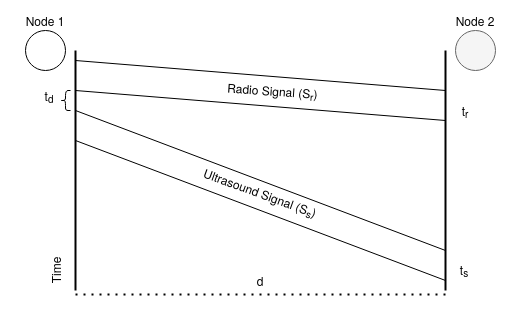
\includegraphics[width=\linewidth]{../Photos/tdoa-timing.png}
      {(b) Multiple signals - single receiver}
    \end{minipage}
    \hfill \break
    \decoRule
    \caption[Time Difference of Arrival cases]{Time Difference of Arrival cases}
    \label{fig:Time-Difference-of-Arrival-cases}
\end{figure}


Η πρώτη περίπτωση σχετίζεται με single signal και multiple receivers και παρουσιάζεται στο 
Figure \ref{fig:Time-Difference-of-Arrival-cases} (a), 
η οποία χρησιμοποιείται συνήθως στα cellular network και απαιτεί την ύπαρξη 
τουλάχιστον 4 beacons για τον υπολογισμό της θέσης ενός free node στον τρισδιάστατο χώρο. Υπολογίζει την χρονική διαφορά
που έφτασε σε καθένα από τα beacons το σήμα που έστειλε το free node, για τον υπολογισμό της απόστασης του free node από
το καθένα από αυτά. Σημαντικό σε αυτήν την περίπτωση είναι και εδώ, να είναι απόλυτα συγχρονισμένα τα beacons. 
Βασίζεται στις ιδιότητες των υπερβολικών καμπύλων και στο ότι με δεδομένη μία συγκεκριμένη χρονική διαφορά του σήματος, 
το free node θα πρέπει να βρίσκεται κάπου πάνω σε μία υπερβολική καμπύλη όπως παρουσιάζεται από το Figure \ref{fig:TDoA-hyberbolas}
\cite{youtube-angle-of-arrival-tdoa-hyberbolas}. 

\begin{figure} [H]
	\centering
	% -----------------
    \begin{minipage}{.5\textwidth}
      \centering
      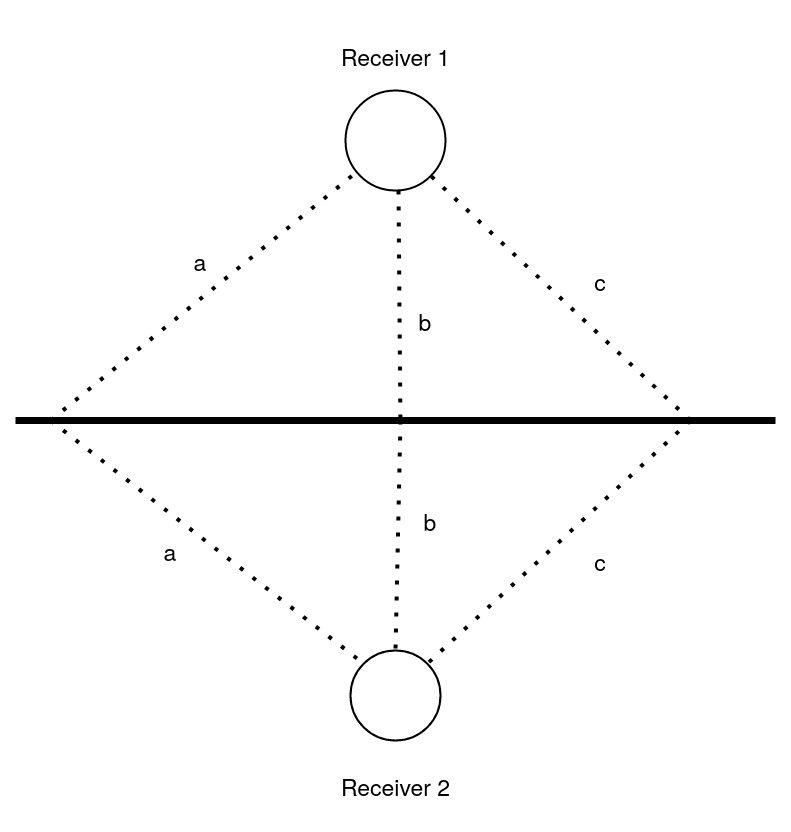
\includegraphics[width=0.5\linewidth]{../Photos/tdoa-dt-0.png}\\
      {(a) $Δt = 0$}
    \end{minipage}%
    % -----------------
    \begin{minipage}{.5\textwidth}
      \centering
      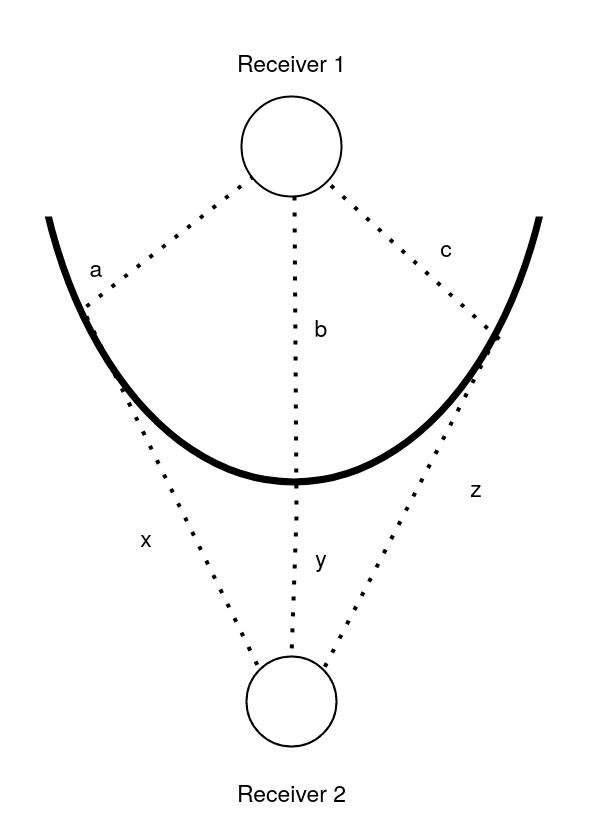
\includegraphics[width=0.5\linewidth]{../Photos/tdoa-dt-not-0.png}\\
      {(b) $Δt \neq 0$}
	\end{minipage}
	% -----------------
    \hfill \break
    \decoRule
    \caption[TDoA hyberbolas based on $\Delta t$]{TDoA hyberbolas based on $\Delta t$}
    \label{fig:TDoA-hyberbolas}
\end{figure}
\begin{align}
	\Delta t = a-a = 0 \quad \quad & \quad \quad\Delta t = x-a \nonumber \\
	\Delta t = b-b = 0 \quad \quad & \quad \quad\Delta t = y-b \nonumber \\
	\Delta t = c-c = 0 \quad \quad & \quad \quad\Delta t = z-c \nonumber
\end{align}


Η γενική ιδέα σε αυτήν την περίπτωση περιγράφεται στην εξίσωση (\ref{eq:tdoa-multiple}) \cite{wsn-Localization-techniques} \cite{simple-tdoa} - και αυτό που 
θέλουμε, είναι να υπολογίσουμε την θέση του $r_t$ (free node) γνωρίζοντας για κάθε δύο διαφορετικά $r_i$ και $r_j$ beacon nodes
την χρονική στιγμή $t_i$ και $t_j$ που έφτασε το σήμα στο καθένα - εάν αυτό κινούταν με ταχύτητα s και το $\norm{\cdot}$ αναπαριστά την ευκλείδεια
απόσταση μεταξύ τους.

\begin{align}
	\Delta t_{ij} \triangleq & t_i - t_j = \frac{1}{s} (\norm{r_i - r_t} - \norm{r_j - r_t}), \quad i \neq j\label{eq:tdoa-multiple}
\end{align}

Η δεύτερη εκδοχή της χρήσης \hyperref[abbr:TDoA]{TDoA} - η οποία είναι πιο συχνή στα \hyperref[abbr:WSN]{WSN} και μας ενδιαφέρει περισσότερο, 
χρησιμοποιεί multiple signals με single receiver και παρουσιάζεται στο Figure \ref{fig:Time-Difference-of-Arrival-cases} (b). 
Αρχή λειτουργίας έχει ότι ο transmitter θα στείλει πολλαπλά διαφορετικού είδους σήματα και ο δέκτης θα μετρήσει την χρονική διαφορά 
που τα έλαβε. Ως παράδειγμα μπορεί το ένα σήμα να είναι σε \hyperref[abbr:RF]{RF} και να κινείται με ταχύτητα $s_r=c_o$ και το άλλο 
ηχητικό με ταχύτητα $s_s \approx 340m/s$. Αν $t_1$ τη χρονική στιγμή που λαμβάνει το \hyperref[abbr:RF]{RF} σήμα ενώ $t_2$ το ηχητικό,
μπορούμε να υπολογίσουμε την απόσταση μεταξύ των κόμβων από την εξίσωση (\ref{eq:tdoa-distance})
\cite{wsn-Localization-systems}.

\begin{align}
	d=&(s_r-s_s)(t_2-t_1) \label{eq:tdoa-distance}
\end{align}

Θετικό σε αυτήν την μέθοδο είναι ότι το error μπορεί να είναι της τάξης των μερικών εκατοστών, όμως αρχικά απαιτεί επιπλέον εξοπλισμό στο node -
ώστε να μπορεί να στείλει και να λάβει πολλαπλά είδη σήματος - πράγμα που μπορεί να το κάνει αντιοικονομικό ή αρκετά μεγαλύτερο σε διαστάσεις από 
το επιθυμητό. Όπως επίσης - και μάλιστα  
σημαντικότερο - η απόσταση η οποία μπορεί να 
χρησιμοποιηθεί, επηρεάζεται σε μεγάλο βαθμό από τα χαρακτηριστικά του δεύτερου σήματος. Ως παράδειγμα τα ηχητικά σήματα 
δεν μπορούν να μεταφερθούν σε μεγάλες αποστάσεις ή το ότι η ταχύτητα τους μπορεί να επηρεαστεί σημαντικά από περιβαλλοντολογικούς παράγοντες
\cite{farooqiazam2016location}.



%----------------------------------------------------------------------
% \subsubsection{Lighthouse}


%----------------------------------------------------------------------
\subsection{Angle}\label{sec:Chapter2-1-1}
Άλλη μία χρήσιμη μέτρηση η οποία μας ενδιαφέρει, είναι η εκτίμηση της γωνίας από την οποία λαμβάνουμε το σήμα ενός γειτονικού
node σε σχέση με έναν άξονας αναφοράς. Ο άξονας αυτός μπορεί να είναι είτε κοινώς για όλα τα nodes (π.χ. ως προς το βόρειο γεωγραφικό πόλο),
είτε μπορεί να είναι για το κάθε node ξεχωριστός, ως παράδειγμα με βάση τον προσανατολισμό του ίδιου του node ή με βάση την γωνία λήψης ενός 
επιπλέον σήματος \cite{wsn-Localization-systems}. Την πληροφορία αυτή την βρίσκουμε στην βιβλιογραφία να ονομάζεται Angle of Arrival 
(\hyperref[abbr:AoA]{AoA}) ή Direction of Arrival (\hyperref[abbr:DoA]{DoA}). 
Γνωρίζουμε ότι ένα σήμα καθορίζεται πλήρως από τρεις παραμέτρους, το πλάτος, την συχνότητα και την φάση του. Για τον υπολογισμό 
της γωνίας (\hyperref[abbr:AoA]{AoA}) μπορούν να χρησιμοποιηθούν τεχνικές με γνώμονα το καθένα από αυτά ξεχωριστά.


\begin{figure} [H]
	\centering
	
    % -----------------
		\begin{minipage}{.5\textwidth}
			\centering
			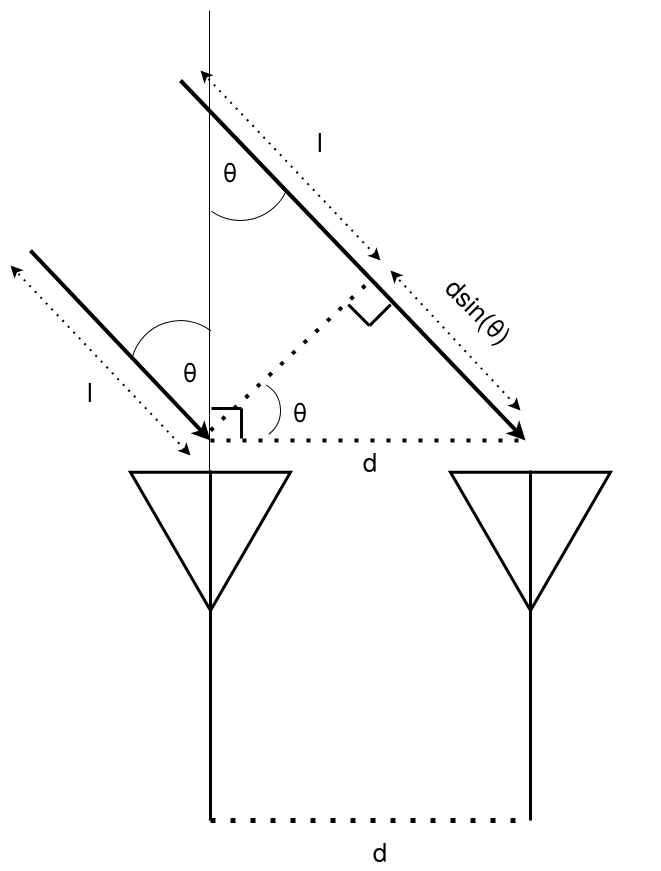
\includegraphics[width=0.6\linewidth]{../Photos/aoa-2antennas.png}\\
			{(a) }
		\end{minipage}%
		% -----------------
		\begin{minipage}{.5\textwidth}
			\centering
			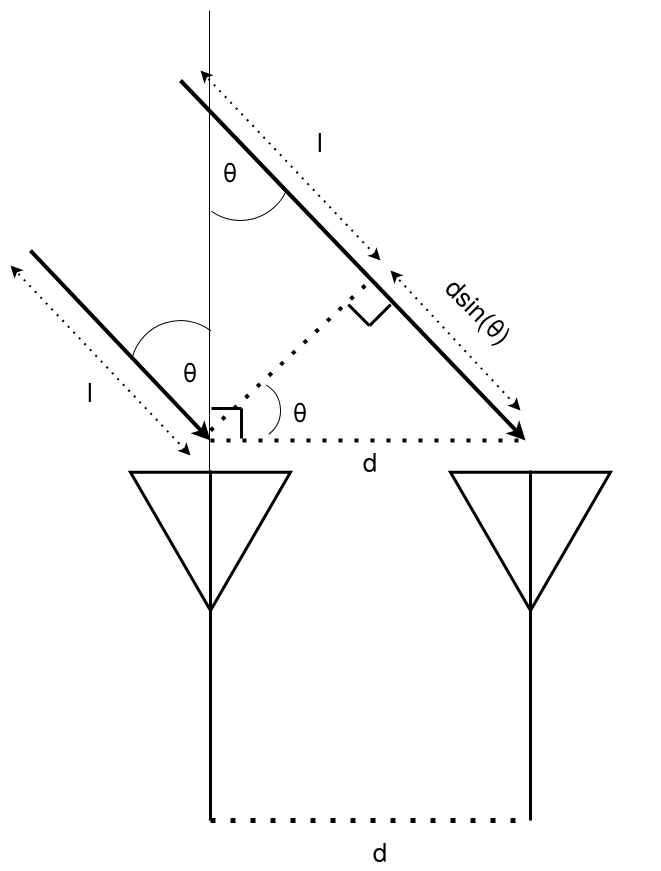
\includegraphics[width=0.6\linewidth]{../Photos/aoa-2antennas.png}\\
			{(b) }
		\end{minipage}
	% -----------------
    \hfill \break
    \decoRule
    \caption[]{}
    \label{}
\end{figure}

TODO: Angle of Arrival

%----------------------------------------------------------------------------------------
%	SECTION 2
%----------------------------------------------------------------------------------------
\section{Position Computation} \label{sec:Chapter2-2} 
Αν έχουμε δύο nodes, οι μετρήσεις που λάβαμε από το Section \ref{sec:Chapter2-1} είναι αρκετές για να γνωρίζουμε την θέση του καθενός,
συνεπώς ενδιαφέρον βρίσκεται στην ύπαρξη τριών ή παραπάνω nodes σε ένα σύστημα. Με βάση τις πληροφορίες που έχουμε συλλέξει - μέσω των τεχνικών που 
περιγράφτηκαν στο προηγούμενο κεφάλαιο - θα προσπαθήσουμε πλέον να εκτιμήσουμε την θέση ενός node. Στην συνέχεια αυτού του section περιγράφονται μέθοδοι οι οποίοι μπορούν να χρησιμοποιηθούν για να το επιτύχουν
αυτό. Κύρια διαφορά τους είναι η απόδοση που μπορεί να έχουν, η οποία όμως σχετίζεται με την αύξηση της πολυπλοκότητας στους υπολογισμούς που θα
χρειαστούν καθώς επίσης και ποιες από τις παραπάνω πληροφορίες θα εκμεταλλευτούν. 

Για την εύρεση της θέσης ενός unknown node στο τρισδιάστατο χώρο $(\mathfrak{R}^3)$ ως ελάχιστο χρειαζόμαστε τέσσερα επιπλέον nodes.
Στις παρακάτω περιγραφές όμως, και χωρίς βλάβη της γενικότητας θα χρησιμοποιηθούν τρία για την απλούστευση της περιγραφής, με την παραδοχή ότι μας
ενδιαφέρει η δισδιάστατη ανάλυση $(\mathfrak{R}^2)$.

\begin{figure} [H]
	\centering
	
    % -----------------
		\begin{minipage}{.33\textwidth}
			\centering
			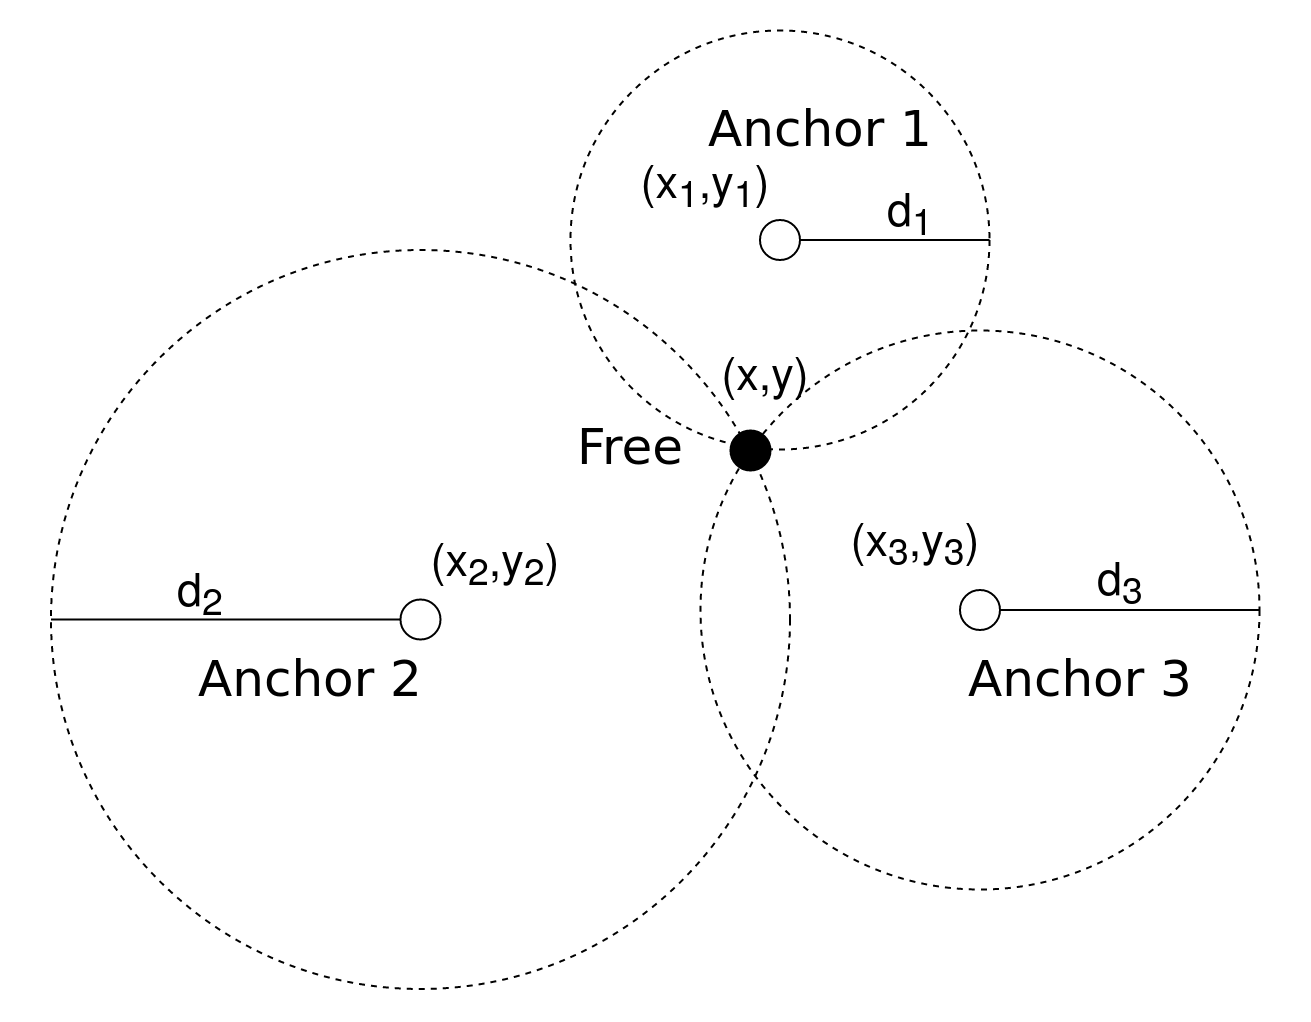
\includegraphics[width=\linewidth]{../Photos/Trilateration-ideal.png}
			{(a) Ideal Trilateration}
		\end{minipage}%
		% -----------------
		\begin{minipage}{.33\textwidth}
			\centering
			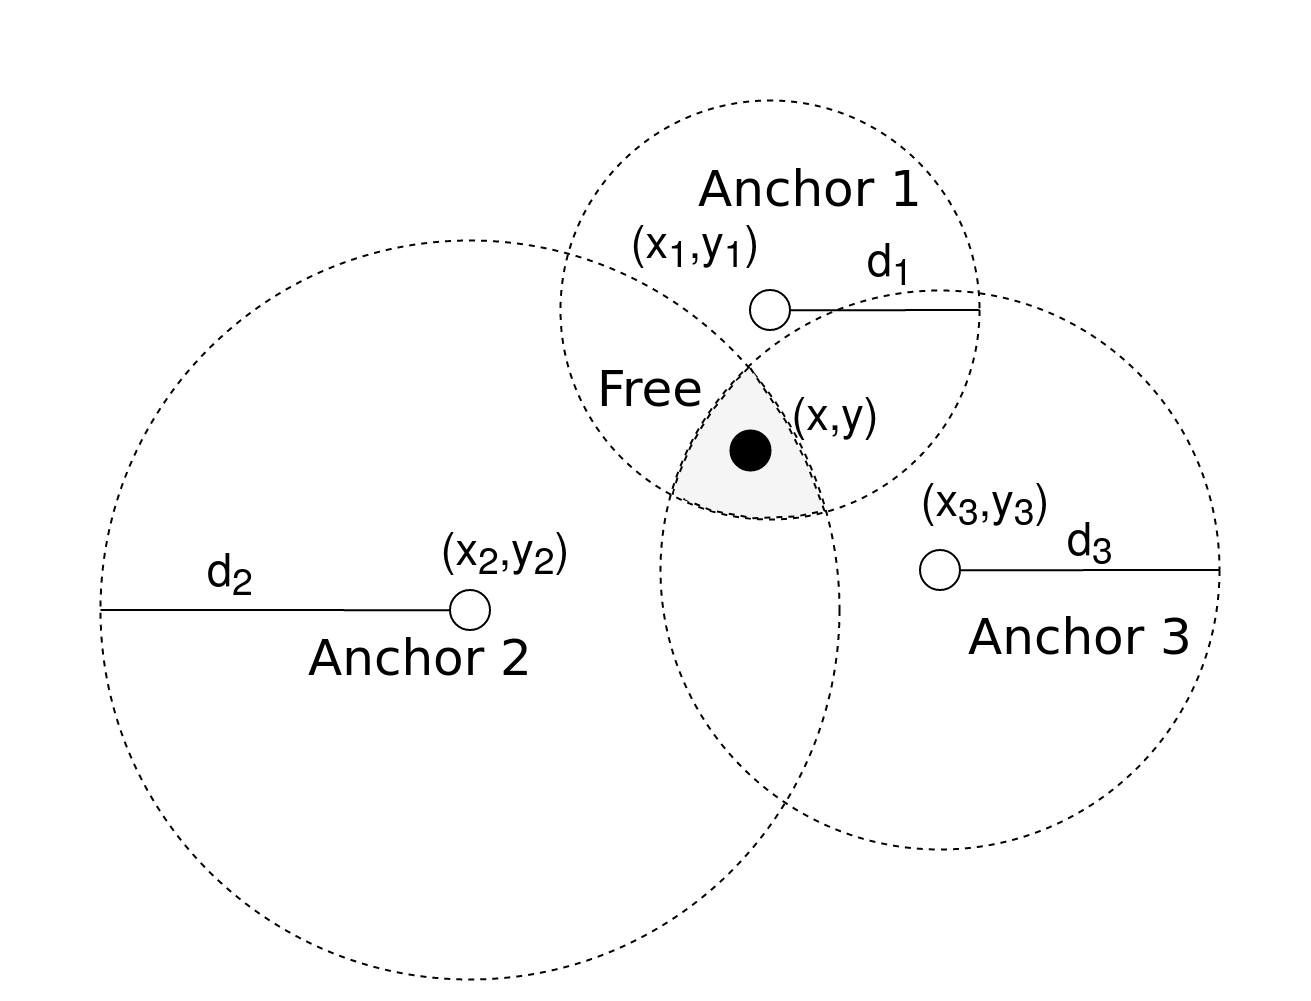
\includegraphics[width=\linewidth]{../Photos/Trilateration-actual.png}
			{(b) Realistic Trilateration}
		\end{minipage}
		% -----------------
		\begin{minipage}{.33\textwidth}
			\centering
			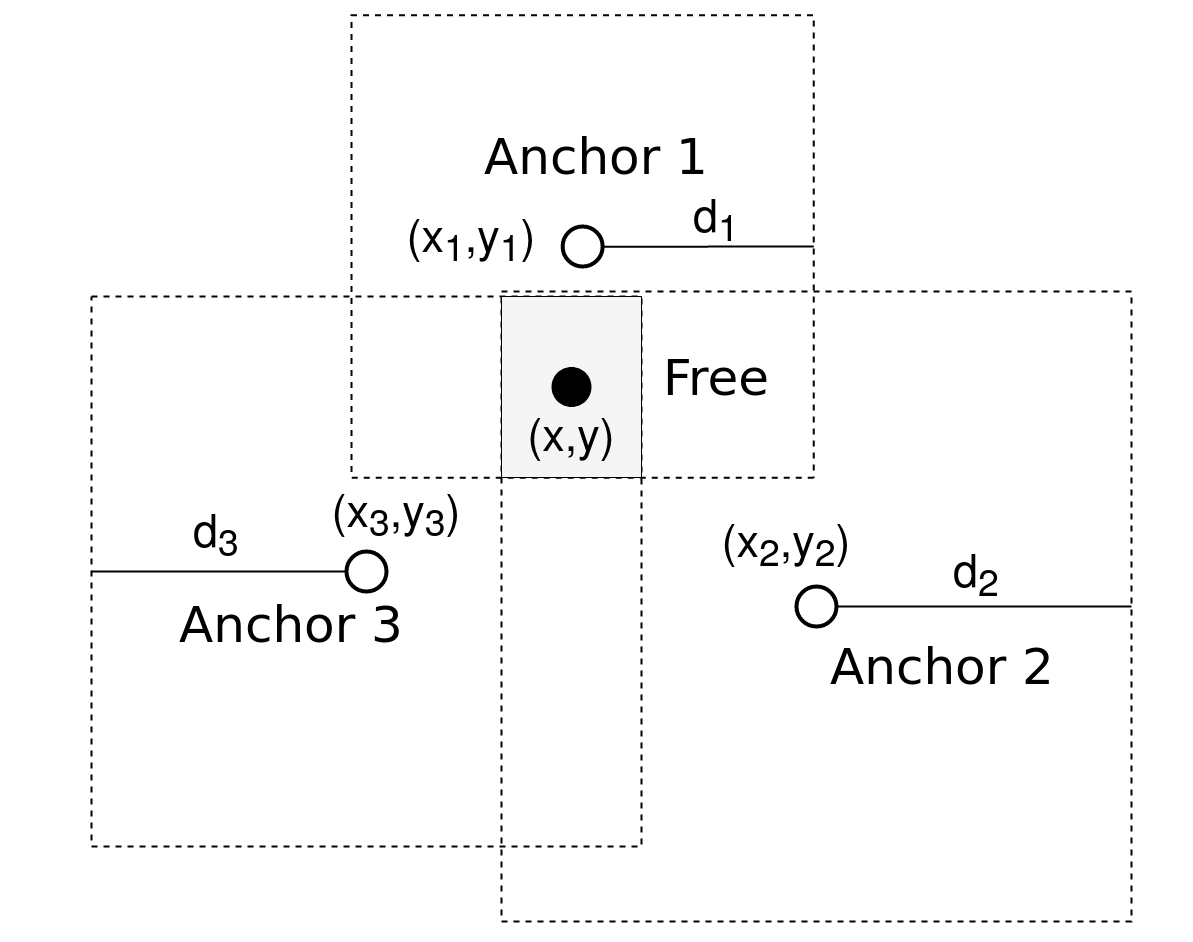
\includegraphics[width=\linewidth]{../Photos/Bounding-box.png}\\
			{(c) Bounding Box}
		\end{minipage}
	% -----------------
    \hfill \break
    \decoRule
    \caption[Position Computation using distance]{Position Computation using distance}
    \label{fig:Position-Computation-using-distance}
\end{figure}

%----------------------------------------------------------------------
\subsubsection{Trilateration}
Η συγκεκριμένη μέθοδος είναι ίσως η πιο απλή διαισθητικά, βασίζεται στην γεωμετρία κύκλων, είναι αυτή που χρησιμοποιείται από τα \hyperref[abbr:GPS]{GPS}
για τον υπολογισμό θέσης \cite{trilateration-vs-triangulation-video}, ενώ αξιοποιεί μόνο πληροφορία απόστασης και όχι γωνίας \cite{Trilateration-vs-Triangulation}.
Η εξίσωση ενός κύκλου από την γεωμετρία γνωρίζουμε ότι περιγράφεται από την εξίσωση (\ref{eq:trilateration-circles}) όπου $(x_i,y_i)$ οι συντεταγμένες
του κέντρο του κύκλου με ακτίνα $d_i$.

\begin{align}
	(x-x_i)^2 + (y-y_i)^2 &= d_i^2 \label{eq:trilateration-circles}
\end{align}

Εάν χρησιμοποιούμε omnidirectional κεραίες \cite{Omnidirectional-antenna} ή στην γενικότερη περίπτωση το μοντέλο της isotropic antenna \cite{Isotropic-radiator} και υπολογίσουμε την απόσταση ενός beacon από το node στο οποίο θέλουμε να υπολογίσουμε την θέση του -
τότε μπορούμε να συμπεράνουμε ότι το free node είναι κάπου πάνω στην περιφέρεια ενός 
κύκλου, με κέντρο το beacon και ακτίνα την απόσταση μεταξύ του beacon και του free node. 
Επαναλαμβάνοντας αυτό για ακόμα δύο beacons, τελικά το free node στο δισδιάστατο επίπεδο $(\mathfrak{R}^2)$ θα πρέπει να βρίσκεται στην τομή των τριών κύκλων, πράγμα που γραφικά 
απεικονίζεται στο Figure \ref{fig:Position-Computation-using-distance} (a) \cite{RSSI-trilateration-Range_based}.

\begin{align}
	x^2-2 x_1 x + x_1^2 + y^2-2 y_1 y + y_1^2 &= d_1^2 \label{eq:trilateration-b1} \\ 
	x^2-2 x_2 x + x_2^2 + y^2-2 y_2 y + y_2^2 &= d_2^2 \label{eq:trilateration-b2} \\
	x^2-2 x_3 x + x_3^2 + y^2-2 y_3 y + y_3^2 &= d_3^2 \label{eq:trilateration-b3} 
\end{align}

Οι εξισώσεις (\ref{eq:trilateration-b1}), (\ref{eq:trilateration-b2}) και (\ref{eq:trilateration-b3}) περιγράφουν πλήρως τους κύκλους του κάθε node από το παράδειγμα 
του Figure \ref{fig:Position-Computation-using-distance} (a),
όπου $(x_i,y_i)$ το κέντρο του κύκλου, $d_i$ η ακτίνα του - για κάθε beacon $i=1,2,3$ και τελικά $(x,y)$ οι συντεταγμένες του free nodes τις οποίες και ψάχνουμε. 
Ένας τρόπος να υπολογίσουμε τις συντεταγμένες αυτές είναι να αφαιρέσουμε από την (\ref{eq:trilateration-b2}) την (\ref{eq:trilateration-b1}) και όμοια από την 
(\ref{eq:trilateration-b3}) την (\ref{eq:trilateration-b2}) ώστε να καταλήξουμε στις παρακάτω δύο εξισώσεις \cite{trilateration-equations} \cite{localization-algorithms-for-wsn}.

\begin{align}
	(-2x_1+2x_2)x + (-2y_1+2y_2)y = d_1^2 - d_2^2 - x_1^2 + x_2^2 - y_1^2 + y_2^2  \nonumber \\
	(-2x_2+2x_3)x + (-2y_2+2y_3)y = d_2^2 - d_3^2 - x_2^2 + x_3^2 - y_2^2 + y_3^2  \nonumber
\end{align}

Ο λόγος που κάναμε το παραπάνω βήμα είναι διότι πλέον έχουμε ένα σύστημα με δύο εξισώσεις και δύο αγνώστους, οπότε μπορούμε εύκολα να θεωρήσουμε τους παρακάτω πίνακες.

\begin{align}
	A = \begin{bmatrix} -2x_1+2x_2 & -2y_1+2y_2 \\ -2x_2+2x_3 & -2y_2+2y_3 \end{bmatrix} \nonumber \quad
	X = \begin{bmatrix} x \\ y \end{bmatrix} \nonumber \quad
	B = \begin{bmatrix} d_1^2 - d_2^2 - x_1^2 + x_2^2 - y_1^2 + y_2^2 \\ d_2^2 - d_3^2 - x_2^2 + x_3^2 - y_2^2 + y_3^2 \end{bmatrix} \nonumber
\end{align}

Με την χρήση των οποίων καταλήγουμε ότι έχουμε να λύσουμε το γραμμικό σύστημα πινάκων που περιγράφεται από την εξίσωση (\ref{eq:trilateration-linear-system}) για τον
υπολογισμό των συντεταγμένων $(x,y)$ του free node οι οποίες μας ενδιαφέρουν.

\begin{align}
	AX = B \label{eq:trilateration-linear-system}
\end{align}

Όπως αναφέρθηκε και στις προηγούμενες ενότητες, ο υπολογισμός της απόστασης πολύ πιθανόν να περιλαμβάνει μια μικρή απόκλιση $\widehat{d_i} = d_i - ε$, 
με το ε συχνά να θεωρείται μία ανεξάρτητη κανονική τυχαία μεταβλητή με μηδενικό μέσο. Αυτό σημαίνει ότι
τότε οι κύκλοι δεν έχουν ένα κοινό σημείο τομής, αλλά το free node βρίσκεται κάπου μέσα στο χωρίο επικάλυψης
των τριών κύκλων, σχηματικά αυτό παρουσιάζεται στο Figure \ref{fig:Position-Computation-using-distance} (b) και σε αυτήν την περίπτωση καταλήγουμε σε ένα
μη πεπερασμένο πλήθος λύσεων, με τη συνάρτηση του κάθε κύκλου να περιγράφεται από την εξίσωση
(\ref{eq:trilateration-circles-error}) \cite{wsn-Localization-systems}.

\begin{align}
	(x-x_i)^2 + (y-y_i)^2 &= d_i^2-e \label{eq:trilateration-circles-error}
\end{align}

Το αρνητικό με αυτήν την μέθοδο, είναι η ανάγκη πραγματοποίησης floating point operations για τον υπολογισμό των συντεταγμένων $(x,y)$ σε πραγματικές συνθήκες - όπου το πλήθος
των οποίων εξαρτάται από τον τρόπο που θα επιλέξουμε να επιλύσουμε το σύστημα. 
Ένας από της μεθόδους επίλυσης της γραμμικής εξίσωσης είναι μέσω του least square method, όπου τότε το πλήθος των floating point operations
που απαιτούνται είναι $(m+n/3)n^2$ με $m$ τον αριθμό των αγνώστων και $n$ τον αριθμό των δοθέντων εξισώσεων \cite{wsn-Localization-systems}.

%----------------------------------------------------------------------
\subsubsection{Bounding Box}
Σε αυτήν την μέθοδο χρησιμοποιούνται τετράγωνα αντί για κύκλους του Trilateration, ενώ και εδώ θεωρούμε $(x_i,y_i)$
τις συντεταγμένες των beacon και $d_i$ η απόσταση που έχουμε υπολογίσει από το free node - για κάθε beacon $i$. Δημιουργούμε
τετράγωνα μήκος πλευράς $2d_i$ με κέντρο το κέντρο του beacon και συντεταγμένες $(x_i - d_i, y_i - d_i)$ \& $(x_i + d_i, y_i + d_i)$. 
Θετικό πλέον είναι ότι δεν χρειάζεται να κάνουμε floating point operations για τον υπολογισμό του χωρίου τομής - αλλά μπορούμε να το υπολογίσουμε
με απλή γεωμετρία. Αφού έχουμε υπολογίσει το χωρίο τομής των τετραγώνων μπορούμε να θεωρήσουμε ότι στο κέντρο του βρίσκεται το free node.
Παράδειγμα αυτής της μεθόδου βρίσκεται στο Figure \ref{fig:Position-Computation-using-distance} (c).
Η συγκεκριμένη μέθοδος μπορεί να είναι ευκολότερη υπολογιστικά και να απαιτεί λιγότερα processor resources από το Trilateration, όμως ταυτόχρονα 
προκύπτει και μεγαλύτερο σφάλμα απόκλισης \cite{wsn-Localization-systems}.   

%----------------------------------------------------------------------
\subsubsection{Triangulation}
Σε αντίθεση με τις παραπάνω μεθόδους, η τεχνική Triangulation εκτιμάει την θέση του node που μας ενδιαφέρει, χρησιμοποιώντας   

%----------------------------------------------------------------------
\subsubsection{Multilateration}

%----------------------------------------------------------------------
\subsubsection{Probabilistic approaches}


%----------------------------------------------------------------------------------------
%	SECTION 3
%----------------------------------------------------------------------------------------
\section{Localization Algorithm} \label{sec:Chapter2-3} 

%----------------------------------------------------------------------
\subsubsection{Range-based vs Range-free}

%----------------------------------------------------------------------
\subsubsection{Distributed vs Centralized Position Computation}

%----------------------------------------------------------------------
\subsubsection{Relative vs Absolute Positioning}

%----------------------------------------------------------------------
\subsubsection{Indoor vs Outdoor}

%----------------------------------------------------------------------
\subsubsection{One-hop vs Multihop}

%----------------------------------------------------------------------
\subsubsection{With vs Without Infrastructure}
   % Theoretical Background (from WSN)
\chapter{Related Work} % Main chapter title
\label{chap:Chapter3}       % For referencing the chapter elsewhere, use \ref{Chapter3} 
\epigraph{``This is where technology is now, imagine where we can go in the future” }{\textit{Timothy Chung}}

Σε αυτό το κεφάλαιο περιγράφονται τρόποι - από την βιβλιογραφία - με τους οποίους, οι υπάρχουσες εφαρμογές 
από drone swarms επιλύουν το localization problem. 

% \cite{trilateration-application1}
% Some systems have been deployed and tested in real-life scenarios, while others remain theoretical approaches
\section{Thesis Approach}
TODO: As last section of this chapter
\cite{10.5555/3400306.3400339}
\cite{6907551}
\cite{8355093}
\cite{PMID:33348720}
\cite{article5}
\cite{inproceedings}
\cite{inproceedings2}
\cite{8453331}
\cite{4967999}
\cite{inproceedings51}
\cite{trilateration-application1}


\section{Demo: In-flight Localisation of Micro-UAVs using Ultra-Wide Band}
Ultra-Wide
Band (UWB)

IEEE 802.15.4-2011 

distance measurement with a precision down to 10 cm within
a 250 m range

It combines good obstacle penetration, and
resilience to both multi-path effects and interference from
other wireless technologies
Symmetrical Double-
Sided Two-Way Ranging 

% This should be the last section
   % Related Work
\chapter{Διαδικασία Σχεδίασης και Υλοποίησης} % Main chapter title
\label{chap:Chapter4}  % For referencing the chapter elsewhere, use \ref{Chapter4}

% \epigraph{”Our goals can only be reached through a vehicle of a plan, in which we must fervently believe, and upon which we must vigorously act. There is no other route to success." }{\textit{Pablo Picasso}}
\epigraph{”Οι στόχοι μας μπορούν μόνο να έρθουν εις πέρας με την σχεδιάση ενός καλά οργανωμένου πλάνου, στο οποίο πρέπει επίμονα να πιστεύουμε, και το οποίο με σθένος πρέπει να πράτουμε. Δεν υπάρχει άλλος δρόμος για την επιτυχία." }{\textit{Pablo Picasso}}

Στο παρόν κεφάλαιο περιγράφεται η διαδικασία σχεδιασμού και υλοποίησης του \Abbr{MoCap} με χρήση drone swarm συστήματος, που συσχετίζεται η παρούσα διπλωματική. 

Μία high-level προσέγγιση, θα μπορούσε να διαχωρίζει το σύστημα σε τρία διακριτά
υποσυστήματα. Αρχικά το optical, του οποίου αρμοδιότητα είναι το detection, το tra\-cking, καθώς και η εκτίμηση
του range ή γωνίας του αντικειμένου από την camera. Δεύτερο, η λήψη των πληροφοριών από τους αισθητήρες ώστε να προσεγγιστεί η θέση του ίδιου
του drone. Τέλος, ο συνδυασμός των δύο παραπάνω μερών και η χρήση κατάλληλης localization τεχνικής για να βρεθεί η θέση του αντικειμένου
στο \Abbr{3D} χώρο.

Πριν γίνει αναφορά καθενός από τα υποσυστήματα που σχεδιάστηκαν, στην \Fig{high-level-system-block-diagram} παρουσιάζεται ένα block diagram του γενικού συστήματος, το οποίο αποτελείται από τα nodes - δουλειά των οποίων είναι η ανίχνευση του αντικειμένου και εκτίμηση της απόστασης του από αυτά - τα οποία αποστέλλουν στον master του συστήματος όλες τις πληροφορίες που έχουν συλλέξει και είναι αυτός που αναλαμβάνει τον προσδιορισμό της θέσης τελικά του object.

% Image
\FigCaptLabelBasedURL{../Photos/High-level-top-diagram.drawio.png}%
{High level system's block diagram}%{}
{high-level-system-block-diagram}%
<1>%
(https://en.creative.com/p/peripherals/creative-live-cam-sync-1080p)

%----------------------------------------------------------------------
\section{Τεχνολογίες και εργαλεία} \label{sec:design-tools}
Αρχικά θα αναφερθούν συνοπτικά η αρχιτεκτονική στην οποία έγινε επιλογή να επιλυθεί το πρόβλημα,
όπως επίσης και τα εξαρτήματα/αισθητήρια όργανα καθώς και τα λογισμικά τα οποία χρησιμοποιήθηκαν. 

\subsection{Embedded Linux System}
Δύο πολύ δημοφιλείς επιλογές στον χώρο των ενσωματωμένων συστημάτων - ως κεντρικές μονάδες επεξεργασίας - είναι οι πλακέτες Raspberry Pi που κατασκευάζονται από την Raspberry Pi Foundation σε συνεργασία με την Broadcom, καθώς και οι πλακέτες Jetson της Nvidia. Στην \Fig{embedded-linux-systems} ως παράδειγμα παρουσιάζονται ενδεικτικά μία εκδοχή από την κάθε οικογένεια, ενώ στα \Tabl{raspberry-pi-specs} και \Tabl{jetson-nano-specs} τα τεχνικά χαρακτηριστικά της εκάστοτε πλακέτας ως αρχικό σημείο αναφοράς. 

\begin{figure} [H]
	\centering
	% -----------------
    \begin{minipage}{.5\textwidth}
      \centering
      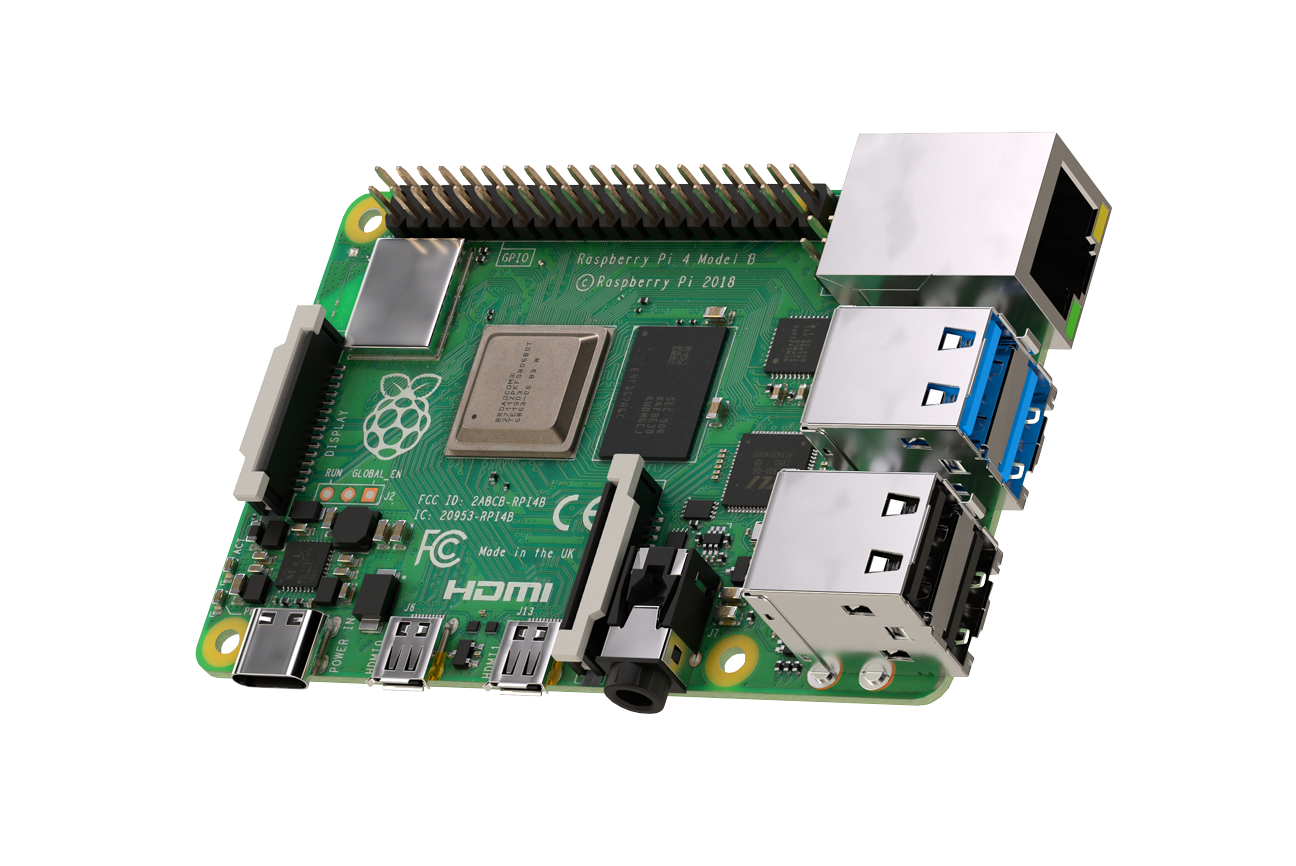
\includegraphics[width=\linewidth]{../Images/Design-Implementation/raspberry-pi-4.png}\\
      {(a) Raspberry Pi 4 \URI{https://www.hellasdigital.gr/go-create/raspberry-and-accessories-el/raspberry-pi/raspberry-pi-4-4gb-ram/}}
    \end{minipage}%
    % -----------------
    \begin{minipage}{.5\textwidth}
      \centering
      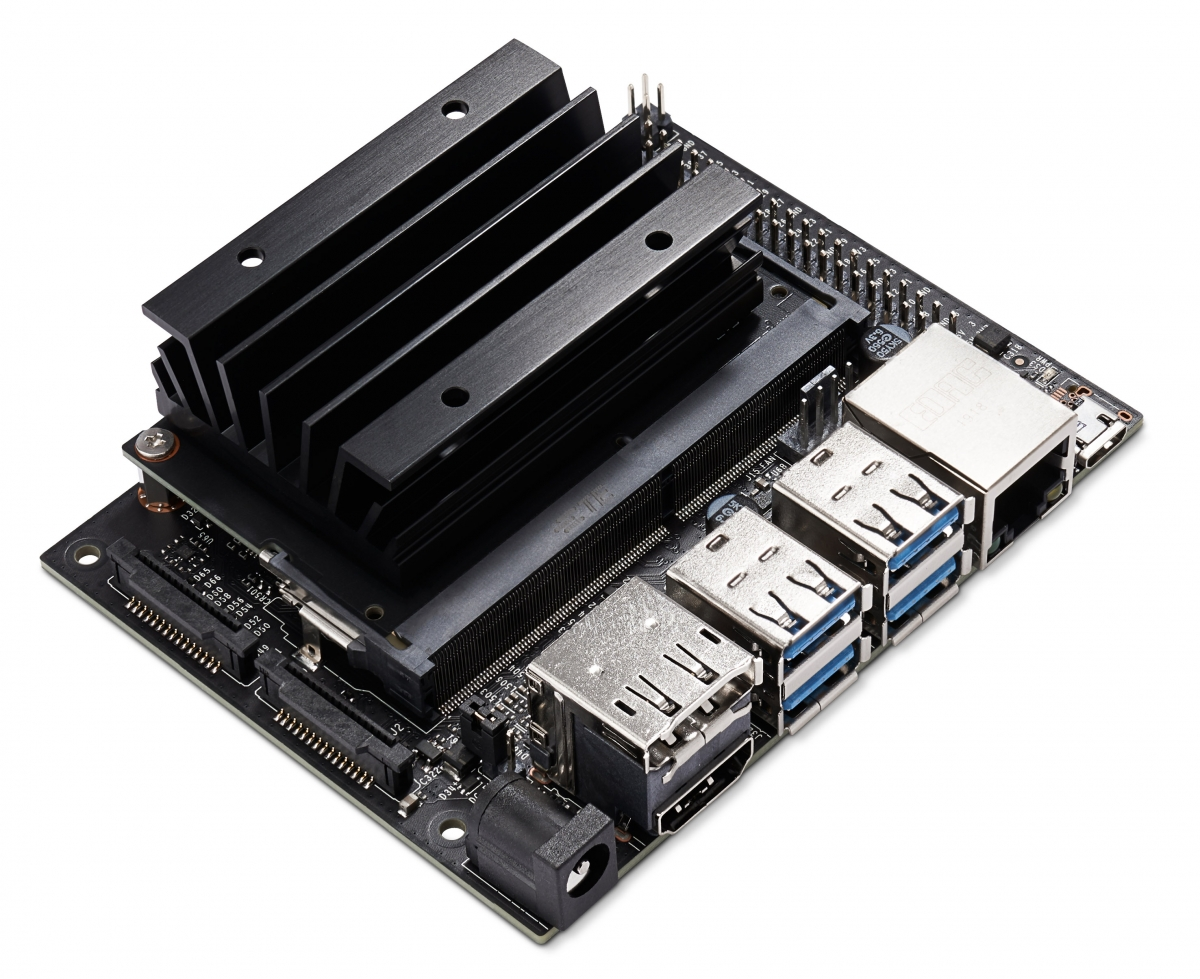
\includegraphics[width=.9\linewidth]{../Images/Design-Implementation/jetson-nano.jpeg}\\
      {(b) Jetson Nano \URI{https://www.hellasdigital.gr/computers/accessories/nvidia-jetson-nano-developer-kit/}}
	\end{minipage}
	% -----------------
    \hfill \break
    \decoRule
    \CaptionBasedwithURL{Υποψήφια Embedded Linux Systems για την υλοποίηση} %\CaptionBasedwithURL{Possible Embedded Linux Systems} 
    \label{fig:embedded-linux-systems}
\end{figure}

Και οι δύο επιλογές αποτελούνται από έναν ARM αρχιτεκτονικής Central Processing Unit (\Abbr{CPU}), ενώ στις Jetson βρίσκεται επιπρόσθετα και ένα Graphics Processing Unit (\Abbr{GPU}) που μπορεί να χρησιμοποιηθεί σε ενσωματωμένα με μεγάλες ανάγκες επεξεργασίας (όπως αυτά που σχετίζονται με εικόνα/βίντεο).

\begin{table}[H]
    \caption[]{Raspberry Pi 4 Model B Specifications}
    \label{tab:raspberry-pi-specs}
    \centering
    \resizebox{.63\textwidth}{!}{
        \begin{tabular}{ll}
            \hline
            \textbf{Feature} & \textbf{Value}  \\
            \hline
                Processor & \Centerstack{Broadcom BCM2711, Quad core Cortex-A72 \\(ARM v8) 64-bit SoC @ 1.5GHz }\\
                Memory & 8GB LPDDR4-3200 SDRAM \\
                Storage & External Micro-SD \\  
                Power & 5V DC (maximum 3A), 5-15Watt \\
                Cost & $\sim$100 €\\
                Weight & 46 grams (without case), 99 grams (with case) \\
                Peripherals & GPIO, I2C, SPI, UART \\
                \hline
        \end{tabular}
    }
  \end{table}

  Στην συγκεκριμένη διπλωματική επιλέχθηκε η ανάπτυξη του συστήματος να γίνει σε Raspberry Pi 4 boards - λόγω του ελάχιστα μικρότερου κόστους καθώς και μάζας τους - έχοντας μελλοντικά την επιλογή για migration ενός ή περισσότερων κόμβων του συστήματος σε Jetson boards, αν κριθεί αυτή η ανάγκη, για λόγους σχετικούς με την ταχύτερη επεξεργασία των δεδομένων.

  \begin{table}[H]
        \caption[]{Jetson Nano Developer Kit Specifications}
        \label{tab:jetson-nano-specs}
        \centering
        \resizebox{.63\textwidth}{!}{
            \begin{tabular}{ll}
                \hline
                \textbf{Feature} & \textbf{Value}  \\
                \hline
                    CPU & Quad-core ARM Cortex-A57 MPCore processor\\
                    GPU & \Centerstack{NVIDIA Maxwell architecture with 128 NVIDIA\\ CUDA® cores} \\
                    Memory & 4 GB 64-bit LPDDR4; 25.6 gigabytes/second \\
                    Storage & External Micro-SD \\  
                    Power & 5V DC, 5-10Watt \\
                    Cost & $\sim$120€\\
                    Weight & 250 grams (without case)\\
                    Peripherals & GPIO, I2C, I2S, SPI, UART \\
                    \hline
            \end{tabular}
        }
      \end{table}

% -----------------

\subsection{ROS} \label{sec:ROS}
Συνδετικός κρίκος των υποσυστημάτων είναι το open-source middleware Robot Operation System (\Abbr{ROS}) \cite{ros} το οποίο 
πε\-ρι\-λα\-μβά\-νει ένα εκτενές σύνολο εργαλείων, βιβλιοθηκών και συ\-μβά\-σεων. Τα πακέτα του οποίου χρησιμοποιούνται για την
λήψη και φιλτράρισμα από τους αισθητήρες των πληροφοριών, επικοινωνία μεταξύ των drone όπως τέλος και 
όποια τρι\-σδιά\-στα\-τη απεικόνιση χρειάζεται.

Μεγάλο πλεονέκτημα του \Abbr{ROS} είναι η ύπαρξη των packages. Τα packages είναι δια\-κρι\-τά αυτόνομα κομμάτια κώδικα τα οποία περικλείουν μία συχνά επαναλαμβανόμενη λογική, συνεπώς μπορούν να χρησιμοποιηθούν αυτούσια - με πολύ εύκολο τρόπο - σε διαφορετικές εφαρμογές χωρίς να υπάρχει η ανάγκη να κάνουμε \textit{reinvent the wheel} κάθε φορά, πετυχαίνοντας με αυτό τον τρόπο το rapid prototyping and testing ενός συστήματος καθώς και την αποφυγή δημιουργίας boilerplate κώδικα δίνοντας έμφαση περισσότερο στο main logic του εκάστοτε συστήματος. 

Το \Abbr{ROS} στην πραγματικότητα είναι ένα meta-operating system, με αποτέλεσμα να χρειάζεται να τρέχει σε ένα πρωτεύον Operating System (\Abbr{OS}), με την μεγαλύτερη συμβατότητά να παρέχεται από διανομές Ubuntu Linux. 

Σημαντικές πηγές που χρησιμοποιήθηκαν για την εκμάθηση του \Abbr{ROS} ήταν κυρίως το documentation του \cite{ros-doc}, καθώς και κάποια από τα external tutorials τα οποία προτείνονται στην παραπάνω σελίδα.

% -----------------
\subsection{Λειτουργικό σύστημα}
Από την στιγμή που επιλέχθηκε να γίνει χρήση του \Abbr{ROS} - που όπως αναφέρθηκε στη \Sect{ROS} προτείνεται ο συνδυασμός του με Ubuntu Linux - έγινε εγκατάσταση στο Raspberry Pi η ειδικά σχεδιασμένη για το αυτό έκδοση Ubuntu Linux 20.04.2 64bit version για ΑRM \cite{ubuntu-raspberry} αρχιτεκτονική. Ουσιαστικά όλες οι λειτουργίες της εφαρμογής θα χρησιμοποιούν το Embedded General Purpose Operating System προκειμένου να λειτουργήσουν, το οποίο σημαίνει ότι αυτό θα είναι κυρίως υπεύθυνο για το scheduling, file-system abstraction, networking, etc. 

% -----------------
\subsection{OpenCV}
Για το οπτικό σκέλος χρησιμοποιήθηκε η ανοιχτού κώδικα βιβλιοθήκη OpenCV \cite{opencv}, η οποία αποτελεί την δημοφιλέστερη επιλογή για real-time Computer Vision related εφαρμογές. Ξεκίνησε η ανάπτυξη της στα εργαστήρια της Intel και έχει ήδη διάρκεια ζωής λίγο περισσότερο από δύο δεκαετίες. Για τις ανάγκες στης συγκεκριμένης ε\-ργα\-σίας χρησιμοποιήθηκε η έκδοση της 4.2.0. Όμοια με το \Abbr{ROS} και για την εκμάθηση του \Abbr{OpenCV}, καθοριστικό ρόλο συνέβαλε η κατανόηση του επίσημου documentation της βιβλιοθήκης \cite{opencv-4-2-0-doc}.

% -----------------
\subsection{Κάμερα}
Σχετικά με την κάμερα, ήταν ανάγκη - όντας πρώτη γενιά του συστήματος -  να επιλεχθεί μία low-cost 1080p camera η οποία θα παρέχει δυνατότητα επιλογής χαμηλότερου resolution για λόγους δοκιμών. Στο πρωτότυπο σύστημα τελικά γίνεται χρήση μία 1080p web cameras της Creative \cite{creative-camera} - \Fig{creative-camera} - με δυνατότητες λήξης βίντεο στα 30fps, η οποία συνδέεται μέσω USB στο Raspberry Pi.

% Image
\FigCaptLabelBasedURL{../Images/Design-Implementation/creative-web-cam.jpeg}%
{Η κάμερα που χρησιμοποιήθηκε για τον εντοπισμό και ανίχνευση του αντικειμένου}%{Camera used for ball detection and tracking}
{creative-camera}%
<0.35>%
(https://en.creative.com/p/peripherals/creative-live-cam-sync-1080p)


% -----------------
\subsection{GPS} \label{sec:GPS}
Παρόλο που - όπως αναφέρθηκε στο \Chap{thesis-approach} - στο συγκεκριμένο σύστημα μας ενδιαφέρει το relative positioning και όχι το absolute, σκεπτόμενοι ότι στην πραγματικότητα το σύστημα σχεδιάζεται με γνώμονα το να λειτουργεί σε outdoor scenarios\udot ένας άμεσος τρόπος προσδιορισμού της θέσης του κάθε drone είναι με χρήση κάποιου εμπορικού αισθητήρα \Abbr{GPS}. Στην συνέχεια και αφού έχει αποκτηθεί πληροφορία απόλυτης θέσης για το κάθε drone μπορεί - θεωρώντας ένα από αυτά ως αρχή των αξόνων - να γίνει translate των απόλυτων συντεταγμένων ώστε να κρατηθεί μόνο πληροφορία σχετικά με την χωρική τοπολογία του δικτύου.

Συγκεκριμένα, χρησιμοποιείται το \Abbr{GPS} για commercial χρήση ΒΝ-220 \cite{bn-220-gps} - \Fig{bn-220-gps} - το οποίο υπόσχεται εμβέλειας ακρίβειας της τάξης των δύο μέτρων. Πρακτικά, παρόλο που για ένα \Abbr{MoCap} σύστημα αυτή η τιμή είναι απαγορευτική, χρησιμοποιείται στα πρώτα versions, καθαρά αναφορικά με την εξικοίωση του τρόπου επικοινωνίας \Abbr{ROS} - \Abbr{GPS}. Σε επόμενα revisions σκοπός είναι η αντικατάσταση του με \Abbr{RTK}-\Abbr{GPS} που συχνά μπορεί να φέρουν drone για αυτήν την χρήση ώστε να φτάσει η συνολική ακρίβεια εκτίμησης της απόλυτης θέσης στα μερικά εκατοστά. 

Το συγκεκριμένο \Abbr{GPS} συνδέεται με το Raspberry Pi μέσω Universal Asynchronous Receiver-Transmitter (\Abbr{UART}) \cite{uart-protocol} σύνδεσης και χρησιμοποιεί NMEA-0183 \cite{NMEA-0183-packets} πακέτα για την επικοινωνία. 

\FigCaptLabelBasedURL{../Images/Design-Implementation/bn220.png}%
{Το GPS που χρησιμοποιήθηκε}%{GPS module used to estimate position}%
{bn-220-gps}%
<0.28>%
(https://www.google.com/imgres?imgurl=https\%3A\%2F\%2Fimages.jdmagicbox.com\%2Fquickquotes\%2Fimages_main\%2Fb07wwx5jvp-electroprime-bn-220-3-0v-5-0v-ttl-level-gnss-module-gps-glonass-dual-gps-module-antenna-v4b2-181504802-qn443.jpg&imgrefurl=https\%3A\%2F\%2Fwww.justdial.com\%2FELECTROPRIME-BN-220-3-0V-5-0V-TTL-Level-Gnss-Module-GPS-Glonass-Dual-GPS-Module-Antenna-V4B2\%2Fpid-181504802&tbnid=YJcAk2WsHSEZiM&vet=10CF8QMyiOAWoXChMI2M3PyrCA8wIVAAAAAB0AAAAAEAk..i&docid=xDxMDFHprlF2iM&w=500&h=500&itg=1&q=bn-220\%20image&hl=el&client=ubuntu&ved=0CF8QMyiOAWoXChMI2M3PyrCA8wIVAAAAAB0AAAAAEAk)

% -----------------
\subsection{IMU}\label{sec:imu}
Ήδη από το \Sect{Chapter1-1-2} έχει γίνει αναφορά για την σημαντικότητα των \Abbr{IMU}, καθώς αποτελούν τα κύρια αισθητήρια όργανα καθορισμού σε πολλαπλούς άξονες της σχετικής θέσης/κίνησης του drone. Επιλέχθηκε να χρησιμοποιηθεί το \Abbr{IMU} \cite{adafruit-10dof-imu} της Adafruit - \Fig{adafruit-10DoF-imu} - το οποίο παρέχει 10-\Abbr{DoF}, με onboard αισθητήρες ένα τριών αξόνων accelerometer, τριών αξόνων gyroscope, τριών αξόνων magnetometer (compass), ένα barometric pressure/altitude αισθητήρα και δυνατότητα υ\-πο\-λο\-γι\-σμού της θερμοκρασίας.

Θετικό του συγκεκριμένου module είναι ότι όλοι οι παραπάνω αισθητήρες είναι συ\-νδε\-δε\-μέ\-νοι σε ένα κοινό Inter-Integrated Circuit (\Abbr{I2C}) \cite{I2C-protocol} bus, μέσω του οποίου μπορεί πολύ εύκολα να γίνει η διασύνδεση με την επεξεργαστική μονάδα που επιθυμούμε και να πραγματοποιηθεί επικοινωνία. 

% Image
\FigCaptLabelBasedURL{../Images/Design-Implementation/10DoF-Adafruit-IMU.jpeg}%
{Adafruit 10 DoF IMU}%
{adafruit-10DoF-imu}%
<0.28>%
(https://www.banggood.com/10DOF-LSM303-L3G4200D-BMP180-Pressure-Sensor-Barometer-Accelerometer-Magnetometer-Gyroscope-Compass-Gyro-Module-p-1660604.html?utm_source=googleshopping&utm_medium=cpc_organic&gmcCountry=GR&utm_content=minha&utm_campaign=minha-gr-en-pc&currency=EUR&cur_warehouse=CN&createTmp=1&utm_source=googleshopping&utm_medium=cpc_bgs&utm_content=sxxx&utm_campaign=sxxx-pla-gr-en-all-purchase-rm-pc-0720&ad_id=534554931006&gclid=Cj0KCQjwv5uKBhD6ARIsAGv9a-zYv4IDUcaDBSG_7ggf1nlFXmcM6l9fHjUUGiwKJGhUsgZsQ_BVn4YaAkG4EALw_wcB)

% -----------------
\subsection{Breakout Board}
Για να λειτουργήσουν τα παραπάνω υποσυστήματα, χρειαζόταν να πραγματοποιηθούν οι κατάλληλες φυσικές διασυνδέσεις. Η απλούστερη εκδοχή θα ήταν να γίνει αυτό με χρήση breadboard, πράγμα όμως που θα πρόσθετε όγκο και βάρος στο τελικό σύστημα, οι οποίοι σε περίπτωση δοκιμών πάνω σε πραγματικά drone να είναι απαγορευτικοί παράγοντες. Συνεπώς, προκειμένου να μπορεί με ευκολία να γίνει η ανάπτυξη του συστήματος, σχεδιάστηκε (στο cad εργαλείο KiCad \cite{KiCad}) και κατασκευάστηκε ένα custom breakout board - το οποίο είναι διαθέσιμο ως open hardware project στο \cite{raspberry-pi-fan-breadkout} - όπως φαίνεται στην \Fig{raspberry-pi-breakout}. Αυτό παρέχει εύκολη πρόσβαση στα GPIO του Raspberry, έξτρα pins για τροφοδοσία στα 5 και 3.3 Volt, pins για τοποθέτηση αισθητήρων - όπως του \Abbr{IMU} - καθώς και mounting holes στα οποία μπορεί να τοποθετηθεί 40x40mm fan για την ψύξη του συστήματος. 

% Image
\FigCaptLabelBasedURL{../Images/Design-Implementation/Rpi-breakout.png}%
{Raspberry Pi breakout}%
{raspberry-pi-breakout}%
<0.4>


% -----------------
\subsection{System Overview}
Η ολοκληρωμένη μορφή του πρωτότυπου συστήματος παρουσιάζεται στην \Fig{thesis-system}, ενώ στο \Tabl{thesis-system-bom} μπορούν να βρεθούν συνολικά τα εξαρτήματα που χρησιμοποιήθηκαν μαζί με την κοστολόγηση τους. 

% Image
\FigCaptLabelBasedURL{../Images/Design-Implementation/thesis-system.jpg}
{Το πρώτυπο σύστημα που σχεδιάστηκε στα πλαίσια της διπλωματικής}%{System designed}%
{thesis-system}%
<0.65>

Το σύστημα ζυγίζει $\sim$ 250gr, μία αρχική εκτίμηση κατανάλωσης είναι τα 15 watt και οι εξωτερικές διαστάσεις του είναι 17x7.5x10.5cm.

\begin{table}[H]
    \caption[]{Bill of Materials}
    \label{tab:thesis-system-bom}
    \centering
    \resizebox{0.55\textwidth}{!}{
        \begin{tabular}{ll}
            \hline
            \textbf{Component} & \textbf{Cost}  \\
            \hline
                Raspberry Pi 4 Model B 8GB & \Centerstack{$\sim$ 100 €}\\
                Creative live cam sync 1080p \cite{creative-camera} & \Centerstack{$\sim$ 44 €}\\
                Adafruit 10 DoF IMU \cite{adafruit-10dof-imu} & \Centerstack{$\sim$ 30 €}\\
                BN-220 GPS Module \cite{bn-220-gps} & \Centerstack{$\sim$ 15 €}\\
                Breakout Board with fan \cite{raspberry-pi-fan-breadkout} & \Centerstack{$\sim$ 8 €}\\
                \hline
        \end{tabular}
    }
  \end{table}


% ------------------------------------------------------------------------------------------------------
\section{Environment}
Έχοντας ήδη αναφερθεί σε όλα τα υποσυστήματα που χρησιμοποιούνται, σε αυτό το section θα δοθεί ο τρόπος με τον οποίο διαμορφώθηκαν/προγραμματίστηκαν ώστε να λειτουργούν μεταξύ τους.

\subsection{Παραμετροποίηση OS} 
Στο \cite{ubuntu-raspi-intall} βρίσκονται αναλυτικές οδηγίες εγκατάστασης του Ubuntu στο Ra\-spbe\-rry Pi, ανάλογα με το λειτουργικό που ήδη χρησιμοποιούμε. Στην συγκεκριμένη περίπτωση - επειδή η εγκατάσταση έγινε από διανομή Linux - αφού έγινε λήψη του pre-made image του Ubuntu, βρέθηκε το path της SD card στον υπολογιστή, στην οποία έγινε umount, και στην συνέχεια χρησιμοποιήθηκε η εντολή dd για την δημιουργία του bootable μέσου, με τον εξής τρόπο.

\begin{lstlisting}[language=sh, escapechar=@, caption={Create bootable SD from Linux},label=create-bootable-sd-terminal]
    @\color{dkgreen}{\$}@ sudo dd bs=4M @if@=PATH_TO_YOUR_IMAGE_FILE of=PATH_TO_YOUR_SD_CARD status=progress
\end{lstlisting}

Μόλις ολοκληρωθεί η παραπάνω διαδικασία, το λειτουργικό σύστημα είναι έτοιμο προς χρήση. Αφού έγινε update του συστήματος, έγιναν οι εξής παραμετροποιήσεις. Αρχικά απενεργοποιήθηκε το Graphical User Interface κατά την διάρκεια του boot, επίσης απενεργοποιήθηκε το auto-suspend μετά από χρονικό διάστημα μη χρήσης, και τέλος εγκαταστάθηκαν οι εφαρμογές/πακέτα/βιβλιοθήκες - όπως το \Abbr{ROS} - που είναι απαραίτητα για την υλοποίηση του συστήματος. 

Σε αυτό το σημείο να αναφερθεί ότι χρησιμοποιήθηκε η έκδοση noetic του \Abbr{ROS}.

% ROS Packages(\TODO{update them}):
% \begin{itemize}
%   \addtolength{\itemindent}{0.3cm}
%   \item tf2\_ros
%   \item robot\_localization
%   \item usb\_cam
%   \item nmea\_navsat\_driver
% \end{itemize}

% -------------------------
\subsection{Επικοινωνία αισθητήρων} 
Αφού ολοκληρώθηκαν οι παραπάνω απαραίτητες ενέργειες, υπήρχε πλέον ένα λειτουργικό περιβάλλον, οπότε και ξεκίνησε η διαδικασία πραγματοποίησης ε\-πι\-τυ\-χη\-μέ\-νης επικοινωνίας με το κάθε υποσύστημα.

%---------------------------
\subsubsection{Σειριακή Επικοινωνία}
Πρώτα θα αναφερθεί η επικοινωνία με το \Abbr{GPS} η οποία όπως αναφέρθηκε στη \Sect{GPS} γίνεται μέσω \Abbr{UART}. Η σειριακή port του Raspberry μπορεί να γίνει access μέσω του αρχείου \textit{/dev/ttyS0}. Ενώ, για να μπορεί να προσπελαστεί από τον χρήστη χρειάστηκε να γίνουν τα βήματα \cite{serial-fix} που υπάρχουν στο \List{fix-serial-communication}.
\newpage
% \begin{enumerate}
%     \item Να προστεθεί η γραμμή `enable\_uart=1' στο αρχείο \textit{/boot/config.txt}
%     \item Να αφαιρεθεί το `console=serial0,115200' από το αρχείο \textit{/boot/firmware/cmdline.txt}
%     \item 
% \end{enumerate}

\begin{lstlisting}[language=bash, escapechar=?, caption={Fix serial communication},label=list:fix-serial-communication]
    # 1. Add `enable_uart=1' to /boot/config.txt file
    sudo bash -c '?echo "enable\_uart=1"? >> /boot/config.txt'

    # 2. Remove `console=serial0,115200' from /boot/firmware/cmdline.txt
    sudo ?sed -e "s/console=serial0,115200//g"? -i /boot/firmware/cmdline.txt

    # 3. Disable serial console service
    sudo systemctl stop serial-getty@ttyS0.service
    sudo systemctl disable serial-getty@ttyS0.service

    # 4. Give privileges to user
    sudo adduser $USER tty
    sudo adduser $USER dialout
    sudo chmod g+r /dev/ttyS0
\end{lstlisting}

Μετά την εκτέλεση τους, συνδέοντας κατάλληλα τα RX - TX του \Abbr{GPS} στο Ra\-spbe\-rry, είναι εφικτό κάνοντας run την εντολή `\textbf{cat /dev/ttyS0}' να έχουμε πρόσβαση στα πακέτα NMEA που στέλνει το \Abbr{GPS}, που έχουν μορφή παρόμοια με το \List{serial-output}.

\begin{lstlisting}[language=bash, escapechar=@, caption={Serial Output, NMEA packets example},label=list:serial-output]
    ...
    $GNGSA,A,1,,,,,,,,,,,,,99.99,99.99,99.99*2E
    $GPGSV,1,1,01,31,,,13*78
    $GLGSV,1,1,00*65
    $GNGLL,,,,,180928.00,V,N*5E
    ...
\end{lstlisting}

Προκειμένου το \Abbr{ROS} να χρησιμοποιεί το \Abbr{GPS}, χρειάστηκε να εγκατασταθεί το πακέτο \textbf{nmea\_navsat\_driver} \cite{nmea-navsat-driver} και παράδειγμα χρήσης αυτού με το \Abbr{ROS} υπάρχει στο \List{gps-ros-sample-usage}.  

\begin{lstlisting}[language=bash, escapechar=@, caption={GPS - ROS sample usage},label=list:gps-ros-sample-usage]
    rosrun nmea_navsat_driver nmea_serial_driver _port:=/dev/ttyS0 _baud:=9600 
\end{lstlisting}

Σημαντικό είναι να αναφερθεί ότι η σειριακή θύρα χρησιμοποιείται για debug λόγους κατά το boot
του Raspberry Pi, συνεπώς το \Abbr{GPS} πρέπει να μην είναι συνδεδεμένο αρχικά και μόνο αφού ολοκληρωθεί το boot να συνδεθεί στο σύστημα.

%---------------------------
\subsubsection{Επικοινωνία I2C}
Σε αντίθεση με την σειριακή επικοινωνία, το \Abbr{IMU} module χρησιμοποιεί το \Abbr{I2C} πρωτόκολλο (βλ. \Sect{imu}).
Για να μπορέσουμε να χρησιμοποιήσουμε το \Abbr{I2C} στο Raspberry, χρειάστηκε να εκτελεστούν οι εντολές που υπάρχουν στη \List{fix-I2C-communication}.

\begin{lstlisting}[language=bash, escapechar=@, caption={Fix I2C communication},label=list:fix-I2C-communication]
    # 1. Install needed library
    sudo apt-get install -y libi2c-dev i2c-tools 

    # 2. Give privileges to user
    sudo adduser $USER i2c
    sudo chmod g+r /dev/i2c-1
\end{lstlisting}

Στην συνέχεια μπορούν να γίνουν οι κατάλληλες συνδέσεις και εκτελώντας την ε\-ντο\-λή `\textbf{i2cdetect -y 1}' έχουμε πρόσβαση στις διευθύνσεις όλων των αισθητήρων που είναι συνδεδεμένες στο \Abbr{I2C} bus, παράδειγμα του output από την εντολή υπάρχει στη \List{I2C-output}\footnote{Το συγκεκριμένο module έχει δοθεί από την Adafruit ως open hardware project, σε περίπτωση που χρησιμοποιηθεί κάποιο replica του, πιθανόν κάποιο address να είναι διαφορετικό}.

\begin{lstlisting}[language=bash, escapechar=@, caption={I2C addressed output example},label=list:I2C-output]
    0  1  2  3  4  5  6  7  8  9  a  b  c  d  e  f
    00:          -- -- -- -- -- -- -- -- -- -- -- -- -- 
    10: -- -- -- -- -- -- -- -- -- 19 -- -- -- -- 1e -- 
    20: -- -- -- -- -- -- -- -- -- -- -- -- -- -- -- -- 
    30: -- -- -- -- -- -- -- -- -- -- -- -- -- -- -- -- 
    40: -- -- -- -- -- -- -- -- -- -- -- -- -- -- -- -- 
    50: -- -- -- -- -- -- -- -- -- -- -- -- -- -- -- -- 
    60: -- -- -- -- -- -- -- -- -- -- -- 6B -- -- -- -- 
    70: -- -- -- -- -- -- -- 77       
\end{lstlisting}

Το μόνο \Abbr{ROS} πακέτο που βρέθηκε \cite{ros-adafruit-10dof-imu-original} - που χρησιμοποιεί αυτό το module - περιείχε κάποια compilation errors. Αφού διορθώθηκαν και προστέθηκαν επιπλέον log messages - το updated repo μπορεί να βρεθεί εδώ \cite{ros-adafruit-10dof-imu-cspyridakis} - ήταν πλέον δυνατό το \Abbr{IMU} να επικοινωνήσει επιτυχώς με το \Abbr{ROS}.

%----------------------------------------------------------------------

\section{Camera} \label{sec:design-implementation-camera}

Πριν αναφερθεί ο τρόπος με τον οποίο χρησιμοποιήθηκε η κάμερα, χρειάζεται πρώτα να μοντελοποιηθεί η πληροφορία που μας παρέχει μία εικόνα. Στην πραγματικότητα όταν μιλάμε για images, ουσιαστικά αναφερόμαστε σε functions που έχουν ως πεδίο ορισμού τα \Abbr{3D} points του χώρου στον οποίο τα λάβαμε, και ως πεδίο τιμών τα \Abbr{2D} projection points που κατέγραψε ο sensor της κάμερας. Για το projection υπάρχουν διάφορα μοντέλα, όπως το Perspective, Weak και Orthographic. Στα πλαίσια της συγκεκριμένης διπλωματικής βασιζόμαστε στο Perspective projection model.

% \begin{table}[H]
%     \caption[Three camera projections]{Three camera projections}
% 	\label{tab:three-camera-projections}
% 	\centering
% 	\resizebox{.8\textwidth}{!}{
% 		\begin{tabular}{lllll}
% 			\toprule
% 			 & & \Centerstack{3D point} & & 2D image\\
% 			\midrule
%             $\imath$. & Perspective: & $(x,y,z)$ & $\rightarrow$ & $\left(\frac{fx}{z}, \frac{fy}{z}\right)$ \\ 
%             $\imath\imath$. & Weak perspective & $(x,y,z)$ & $\rightarrow$ & $\left(\frac{fx}{z_0}, \frac{fy}{z_0}\right)$ \\ 
%             $\imath\imath\imath$. & Orthographic & $(x,y,z)$ & $\rightarrow$ & $(x,y)$ \\ 
% 			\bottomrule
% 		\end{tabular}
% 	}
% \end{table}

% Image
\FigCaptLabelBasedURL{../Photos/pinhole-model.png}%
{Ιδανικό μοντέλο του pinhole}%{Ideal pinhole model}%
{ideal-pinhole-model}%
<0.8>

Επίσης, ένα απλό (για την κάμερα) - παρόλα αυτά αρκετά περιγραφικό και κοντά στην πραγματικότητα - μοντέλο, το οποίο χρησιμοποιείται συχνά για \Abbr{CV} applications είναι αυτό του Pinhole Model, παράδειγμα στην \Fig{ideal-pinhole-model}, με το COP να είναι το Center of Projection και να χρησιμοποιούμε το Virtual Image Plane για τους υπολογισμούς - μαθηματικά ισοδύναμο με το πραγματικό Image Plane - με τη διαφορά του μη ανεστραμμένου ειδώλου.

Μπορούμε να μεταφερθούμε - από ένα κοινό σε όλους - World Coordinate System (${}^{w}\overrightarrow{p}$) στο Coordinate System της κάμερας (${}^{c}\overrightarrow{p}$) μέσω μίας Rotation (${}^{c}_{w}R$) και μίας Translation (${}^{c}_{w}\overrightarrow{t}$) διαδικασίας - \Equa{world-to-camera-frame}. Συχνά τα περιεχόμενα των Rotation κι Translation ονομάζονται από κοινού Extrinsic Parameters.

Ενώ για τη πραγματική μεταφορά από το Camera Coordinate System σε αυτό της εικόνας θα πρέπει να λάβουμε υπόψιν τις φυσικές παραμέτρους της κάμερας όπως το Focal Length, Skew, etc., οι οποίες συνολικά ονομάζονται Intrinsic Parameters. Η σχέση \EqNum{camera-to-image-plane} παρουσιάζει αυτόν τον μετασχηματισμό, με $(u,v)$ τα pixel στην κάμερα, $(x,y,z)$ οι συντεταγμένες του αντικειμένου με βάση το Camera Coordinate System και $(\alpha, \beta, \theta, u_0, v_0)$ τα Intrinsic Parameters.


\begin{gather}
	{}^{c}\overrightarrow{p} \quad = \quad {}^{c}_{w}R \quad {}^{w}\overrightarrow{p} \quad + \quad {}^{c}_{w}\overrightarrow{t} \label{eq:world-to-camera-frame}\\
    \begin{matrix}
        u = \alpha \frac{x}{z} - \alpha cot(\theta)\frac{y}{z} + u_0
    \end{matrix} 
    \quad \quad \quad
    \begin{matrix}
        v = \frac{\beta}{\sin{\theta}} \frac{y}{z} + v_0
    \end{matrix} \label{eq:camera-to-image-plane}
\end{gather}

Οι παραπάνω υπολογισμοί με τη μορφή που είναι αυτή την στιγμή κάνουν πιο δύσκολο τον τρόπο υπολογισμού σε ψηφιακά συστήματα. Επιπλέον έχουν μη γραμμικά μέρη, με αποτέλεσμα να μην είναι αναστρέψιμοι, για αυτόν τον λόγο γίνεται αναφορά των homogeneous coordinates. Τα homogeneous coordinates χρησιμοποιούνται ώστε να μπορούμε να μετασχηματίσουμε εύκολα, σε μία πλέον τις παραπάνω σχέσεις, με χρήση πινάκων - \Equa{world-to-image-trans}. Όπου $x$ οι συντεταγμένες στην εικόνα, $X$ οι συντεταγμένες στον φυσικό κόσμο και $M$ ο πίνακας μετασχηματισμού, τα περιεχόμενα του οποίου αναλύονται στην σχέση \EqNum{world-to-image-matrix} 

\begin{align}
	\begin{matrix}
        (x/w,y/w) \Leftrightarrow \begin{bmatrix} x \\ y \\ w \end{bmatrix} \\ 
        \textrm{homogeneous image} \\ 
        \textrm{(2D) coordinates}
    \end{matrix} 
    \nonumber \quad \quad
    \begin{matrix}
        (x/w,y/w,z/w) \Leftrightarrow \begin{bmatrix} x \\ y \\ z \\ w \end{bmatrix} \\ 
        \textrm{homogeneous scene} \\ 
        \textrm{(3D) coordinates }
    \end{matrix} \nonumber
\end{align}

\begin{gather}
	x \simeq \begin{bmatrix} sx \\ sy \\ s \end{bmatrix} = MX = M \begin{bmatrix} X \\ Y \\ Z  \\ 1 \end{bmatrix} \label{eq:world-to-image-trans}
\end{gather}

\begin{gather}
	M_{3x4} = 
    \begin{matrix}
        \begin{bmatrix} 
            f & s & x'_c \\ 
            0 & af & y'_c \\
            0  & 0 & 1
        \end{bmatrix}\\
        Intrinsics
    \end{matrix}
    \begin{matrix}
        \begin{bmatrix} 
            1 & 0 & 0 & 0 \\ 
            0 & 1 & 0 & 0 \\ 
            0 & 0 & 1 & 0 \\ 
        \end{bmatrix}\\
        Projection
    \end{matrix}
    \begin{matrix}
        \begin{bmatrix} 
            R_{3x3} & 0_{3x1} \\ 
            0_{1x3} & 1 \\  
        \end{bmatrix}\\
        Rotation
    \end{matrix}
    \begin{matrix}
        \begin{bmatrix} 
            I_{3x3} & T_{3x1} \\ 
            0_{1x3} & 1 \\  
        \end{bmatrix}\\
        Translation
    \end{matrix} \label{eq:world-to-image-matrix}
\end{gather}

Ένα αρκετά βοηθητικό Massive Open Online Course (\Abbr{MOOC}) το οποίο βοήθησε ώστε να κατανοηθεί περισσότερο το σκέλος του \Abbr{CV} και στο οποίο μπορεί κάποιος να ανατρέξει για περισσότερες λεπτομέρειες σε σχέση με τους παραπάνω φορμαλισμούς είναι το \cite{introduction-to-computer-vision}. Επιπρόσθετα, στη \Sect{camera-calibration} περιγράφεται ο τρόπος υπολογισμού των στοιχείων του πίνακα μετασχηματισμού $M$.

% ------------------
\subsection{Camera Calibration} \label{sec:camera-calibration}
Στη \Sect{design-implementation-camera} έγινε αναφορά του πίνακα μετασχηματισμού $M$. Επίσης, τα lens μίας κάμερας δεν είναι ιδανικά, κάνοντας τις λήψεις να φέρουν παραμορφώσεις (βλ. \Fig{distortion-types}). Η συνολική παραμόρφωση ενός lens μπορεί να περιγραφεί μέσω των Distortion coefficients. Η διαδικασία υπολογισμού όλων των παραμέτρων της κάμερας - προκειμένου αξιόπιστα να μπορούμε να κάνουμε υπολογισμούς με βάση τις λήψεις της σε μία \Abbr{CV} εφαρμογή - ονομάζεται camera calibration. 

% Image
\FigCaptLabelBasedURL{../Images/Design-Implementation/distortion-types.png}%
{Οι πιο συνηθισμένοι τύποι distortion των φακών}%{Most common distortion types}%
{distortion-types}%
<0.65>%
(https://learnopencv.com/understanding-lens-distortion/)

Στην συγκεκριμένη διπλωματική τυπώθηκε ένα checkerboard pattern, και α\-ξιο\-ποιή\-θη\-καν εργαλεία που υλοποιούν το Zhang's method για τον υπολογισμό των πα\-ρα\-μέ\-τρων. Αρχικά, έγινε προσπάθεια με native τρόπο χρησιμοποιώντας άμεσα το framework \Abbr{OpenCV} να πραγματοποιηθεί το calibration, επειδή όμως κατέληγε σε μεγάλο mean error in pixel - περίπου 3.56 στα πειράματα - αποφασίστηκε να χρησιμοποιηθεί εναλλακτική μέθοδος. Παρόλο που και το \Abbr{ROS} παρέχει πακέτο για το calibration, επιλέχθηκε μέσω του Matlab και χρήση του Camera Calibration toolkit να πραγματοποιηθεί τελικά. Κύριος λόγος διότι σε αυτό παρέχονται επιπρόσθετες πληροφορίες - βλ. \Fig{matlab-useful-graphs} - κατά το calibration, επιτυγχάνοντας τελικά mean error in pixel περίπου 0.25. Αυτή η διαδικασία πραγματοποιήθηκε για αναλύσεις 1920x1080, 1280x720 και 640x480. 

Στο τέλος του calibration, είχαν υπολογιστεί και έγιναν exported τα parameters. Ενώ με τα περιεχόμενα των πεδίων FocalLength, PrincipalPoint, RadialDistortion, TangentialDistortion και Skew δημιουργήθηκαν τα yaml αρχεία που χρειάζεται το \Abbr{ROS} \cite{ros-calibration-instr1} \cite{ros-calibration-instr2}.


\begin{figure} [H]
	\centering
	% -----------------
    \begin{minipage}{.4\textwidth}
      \centering
      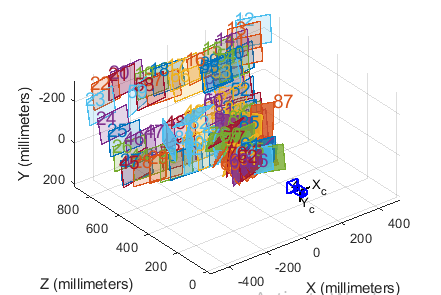
\includegraphics[width=\linewidth]{../Photos/CameraCalibration/1920x1080/calib-samples.png}\\
      {(a) Images in \Abbr{3D} space }
    \end{minipage}%
    % -----------------
    \begin{minipage}{.6\textwidth}
      \centering
      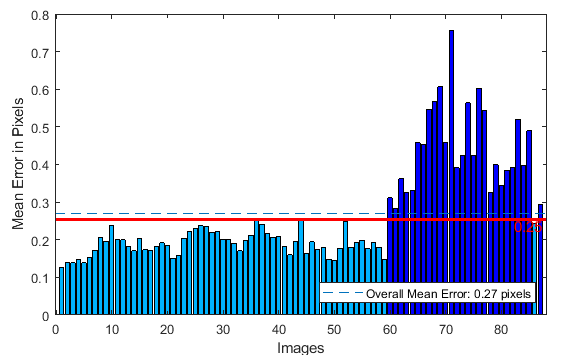
\includegraphics[width=\linewidth]{../Photos/CameraCalibration/1920x1080/calib-mean-error.png}\\
      {(b) Mean Error in pixels per image }
	\end{minipage}
	% ----------------- 
    \hfill \break
    \decoRule
    \CaptionBasedwithURL{Matlab camera toolkit} 
    \label{fig:matlab-useful-graphs}
\end{figure}

% ------------------
\subsection{Χρήση κάμερας} \label{sec:camera-usage}
Προκειμένου να λειτουργεί η κάμερα με το \Abbr{ROS}, χρειάστηκε αρχικά να συνδεθεί μέσω USB με το Raspberry Pi, ενώ χρησιμοποιήθηκε το package \textbf{usb\_cam} για την διαχείριση της. Στο launch αρχείο που δημιουργήθηκε, κατά την εκτέλεση του \textit{/usb\_cam\_node}, γίνεται επιλογή της ανάλυσης που πρόκειται να χρησιμοποιηθεί\udot όπως επίσης μέσω της παραμέτρου \textit{camera\_info\_url}, επιλέγεται το yaml αρχείο με τα χαρακτηριστικά της κάμερας που δημιουργήθηκε κατά το calibration. 

Το \textit{/usb\_cam\_node} κάνει publish στο topic \textit{/usb\_cam/image\_raw} τα περιεχόμενα της κάμερας. Tο \textbf{image\_proc} είναι υπεύθυνο για το undistortion του image ώστε να μπορούν να πραγματοποιηθούν αξιόπιστες μετρήσεις.  Η επεξεργασία του stream της κάμερας γίνεται από το node με όνομα \textit{/worker\_node} που δημιουργήθηκε, το οποίο κάνει subscribe στο topic της undistorted εικόνας, μετασχηματίζει από πακέτα \Abbr{ROS} σε Mat στοιχεία - που χρησιμοποιεί το \Abbr{OpenCV},  μέσω του \textit{cv\_bridge} - και αναλαμβάνει το κομμάτι της \Abbr{CV} επεξεργασίας για της ανάγκες της εφαρμογής. 

\FigCaptLabelBasedURL{../Photos/camera-usage-ros.png}%
{ROS - camera related nodes/topics setup}%{ROS - camera related nodes/topics setup}%
{thesis-camera-nodes-topics-setup}%
<1>

Αρκετές ήταν οι φορές που υπήρχε ανάγκη (για λόγους αποσφαλμάτωσης), σε ο\-πτι\-κό feedback της \Abbr{CV} επεξεργασίας από nodes, που μπορεί να είναι διαφορετικά φυσικά μηχανήματα από αυτά που τρέχει η εφαρμογή. Πράγμα που εύκολα επιλύεται αξιοποιώντας το package \textbf{/web\_video\_server}. Αυτό είναι subscriber στο topic \textit{/usb\_\-cam/processed\_ image} (topic στο οποίο το \textit{/worker\_node} κάνει publish τα αποτελέσματα της επεξεργασίας) ώστε μέσω κάποιου browser να μπορούμε εύκολα να δούμε τα αποτελέσματα της. Η \Fig{thesis-camera-nodes-topics-setup} παρουσιάζει τα topics/nodes που αναφέρθηκαν και τον τρόπο με τον οποίο επι\-κοι\-νω\-νούν.

% ------------------
\subsection{Εντοπισμός Αντικειμένου}
Το αντικείμενο του οποίου η θέση επιλέχθηκε να προσδιοριστεί, είναι μία μπάλα - καθώς μπορεί να προσφέρει ανεξαρτήτου γωνία λήψης ίδια πληροφορία για τις διαστάσεις της - μεγέθους ανάλογη με τις μπάλες ποδοσφαίρου. 
Συνεπώς δεν μας ενδιαφέρει το orientation του αντικειμένου, παρά μόνο το location.

\subsubsection{Με βάση το χρώμα} \label{sec:hsv-detection-sec}

Πρώτη προσπάθεια εκτίμησης της θέσης, ήταν χρησιμοποιώντας ως σημείο αναφοράς το χρώμα της. Έχοντας επιλέξει το χρώμα της μπάλας να είναι διαφορετικό από τα περισσότερα στοιχεία της σκηνής στην οποία την καταγράφουμε, μπορούμε εύκολα να προσδιορίσουμε και την θέση του αντικειμένου στο image plane.

Συχνά οι λήψεις μίας κάμερας αναπαριστάνονται στο RGB color space, αρκετά χρήσιμο όμως είναι η χρήση του HSV για \Abbr{CV} εφαρμογές, με κύριο λόγο τον διαχωρισμό που παρέχεται μεταξύ color information και intensity στο συγκεκριμένο color space. Οπτική αναπαράσταση αυτών βρίσκεται στην \Fig{color-space}. 

\begin{figure} [H]
	\centering
	% -----------------
    \begin{minipage}{.5\textwidth}
      \centering
      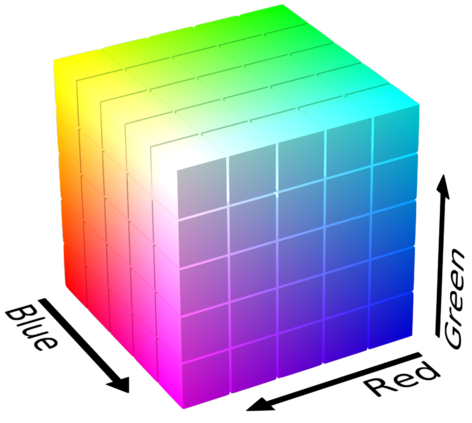
\includegraphics[width=0.5\linewidth]{../Images/Design-Implementation/rgb.png}\\
      {(a) RGB \URI{https://www.google.com/imgres?imgurl=https\%3A\%2F\%2Fqph.fs.quoracdn.net\%2Fmain-qimg-d33e22b88db273d09513f652bcb79736&imgrefurl=https\%3A\%2F\%2Fwww.quora.com\%2FWhat-are-the-differences-between-RGB-HSV-and-CIE-Lab&tbnid=XWOdefD1z2_-gM&vet=12ahUKEwjE5Iacxo_zAhW95LsIHeBlCGYQMygKegUIARCzAQ..i&docid=8mJRsf1Rk3zM_M&w=1600&h=1200&q=rgb\%20vs\%20hsv&hl=el&client=ubuntu&ved=2ahUKEwjE5Iacxo_zAhW95LsIHeBlCGYQMygKegUIARCzAQ}}
    \end{minipage}%
    % -----------------
    \begin{minipage}{.5\textwidth}
      \centering
      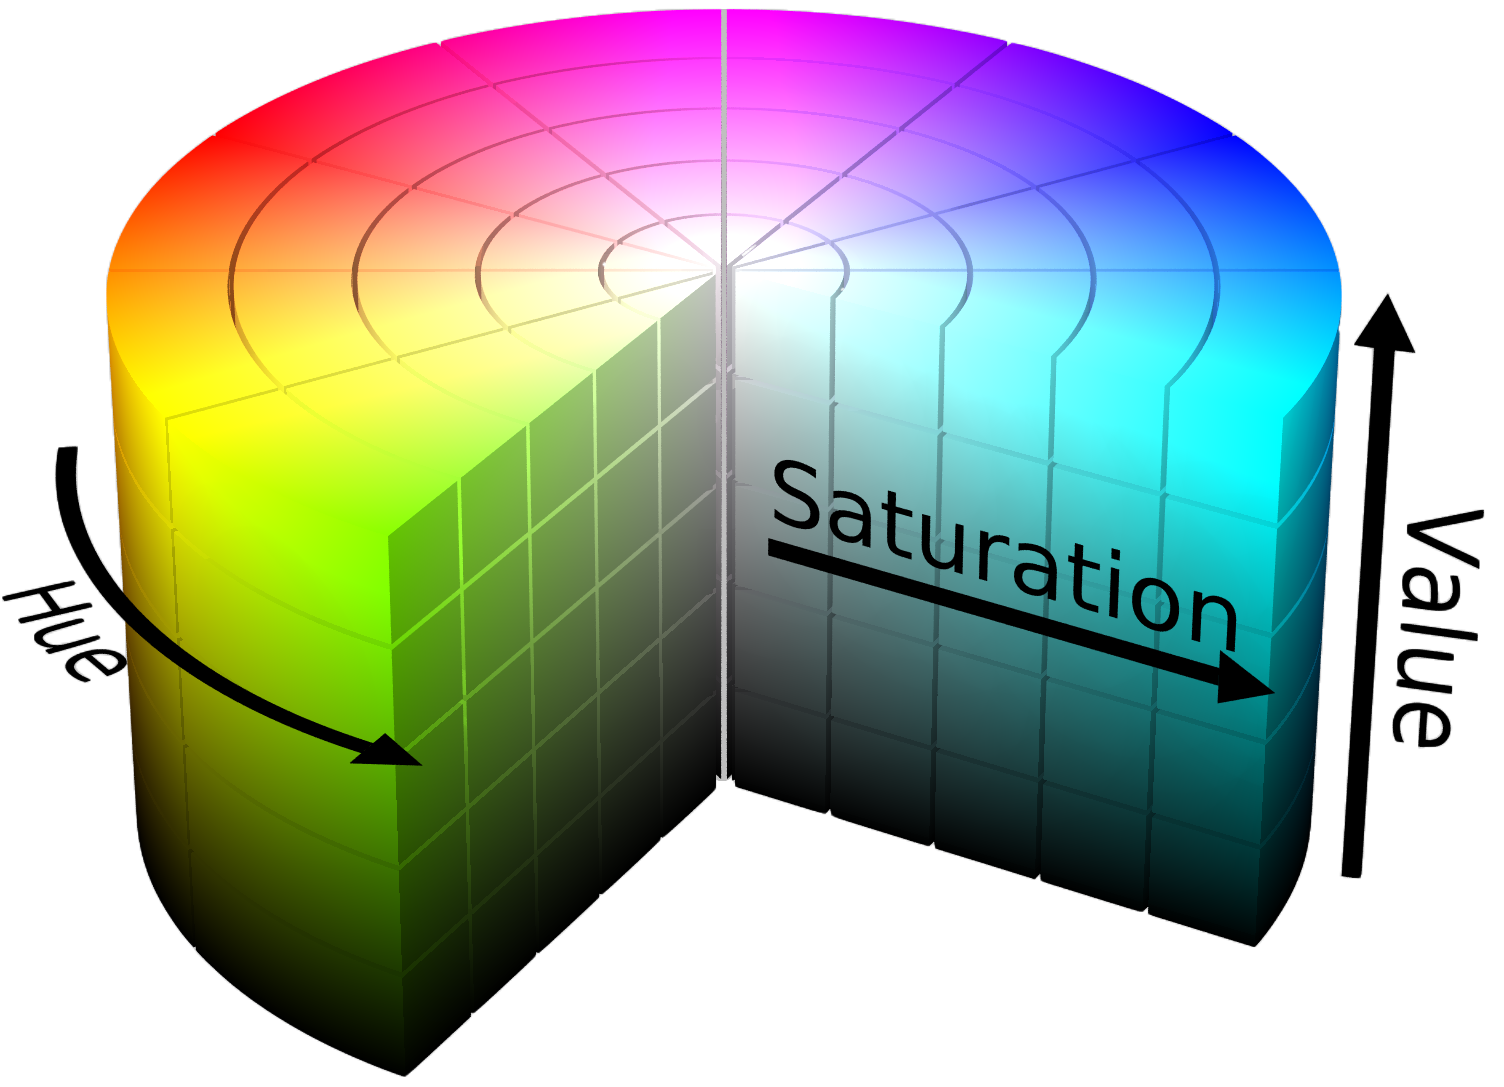
\includegraphics[width=.6\linewidth]{../Images/Design-Implementation/hsv.png}\\
      {(b) HSV \URI{https://www.google.com/imgres?imgurl=https\%3A\%2F\%2Fqph.fs.quoracdn.net\%2Fmain-qimg-7c6685f64cf5ea346a9c33be0d256a95&imgrefurl=https\%3A\%2F\%2Fwww.quora.com\%2FWhat-are-the-differences-between-RGB-HSV-and-CIE-Lab&tbnid=BwsDxAXpjI2MqM&vet=12ahUKEwjE5Iacxo_zAhW95LsIHeBlCGYQMygBegUIARCdAQ..i&docid=8mJRsf1Rk3zM_M&w=1600&h=1200&q=rgb\%20vs\%20hsv&hl=el&client=ubuntu&ved=2ahUKEwjE5Iacxo_zAhW95LsIHeBlCGYQMygBegUIARCdAQ}}
	\end{minipage}
	% -----------------
    \hfill \break
    \decoRule
    \CaptionBasedwithURL{Color Spaces} 
    \label{fig:color-space}
\end{figure}

Στον \Algo{hsv-detect} παρουσιάζεται η διαδικασία που ακολουθήθηκε προκειμένου να ε\-ντο\-πι\-στεί η μπάλα στην σκηνή με βάση το χρώμα της, ενώ στην \Fig{balls-detection-color} εμφανίζονται τα αποτελέσματα από το κάθε επίπεδο επεξεργασίας.

% ALGORITHM
\begin{algorithm}[H]
	\caption[HSV (color based) ball detection]{HSV (color based) ball detection}\label{alg:hsv-detect}
	\begin{algorithmic}[1]
		\Statex{{\bf procedure} detectBall}{}
            \State Define preferable color's limit HSV values
            \State Get one frame of the video
            \State Remove high frequencies from the frame
            \State Convert frame from RGB to HSV color space
            \State Choose only pixels that are in between preferable color's limit values 
	\end{algorithmic}
\end{algorithm}

\FigCaptLabelBasedURL{../Photos/thesis-hsv.png}%
{Ανίχνευση μπάλας με βάση το χρώμα}%{Detect balls based on their color}%
{balls-detection-color}%
<0.9>

Ένα μεγάλο μέρος των \Abbr{CV} εφαρμογών περιλαμβάνει ως διαδικασίες επεξεργασίας το να γίνεται convolution ή cross-correlation\footnote{Η διαφορά μεταξύ του convolution και του cross-correlation, είναι ότι στο convolution ο kernel αναστρέφεται} ενός kernel με τα pixel της εικόνας. Αυτή η διαδικασία - που για το convolution περιγράφεται μαθηματικά από την εξίσωση \EqNum{cross-correlation} και οπτικά από την \Fig{convolution-example} - έχει ποικίλες εφαρμογές οι οποίες διαχωρίζονται με βάση την επιλογή του kernel. Μία εξ' αυτών είναι για λόγους smoothing, που στην συγκεκριμένη περίπτωση περιλαμβάνει σημαντική διαδικασία του preprocessing, καθώς με αυτόν τον τρόπο μειώνουμε την ποσότητα των υψηλών συχνοτήτων συνεπώς και τον θόρυβο στην εικόνα.

\begin{gather}
	O[i,j] = k * I = \sum_{u=-k}^{k} \sum_{v=-k}^{k} k[u,v]I[i-u,j-v] \label{eq:cross-correlation}
\end{gather}

\FigCaptLabelBasedURL{../Images/Design-Implementation/cross-correlation.png}%
{Convolution παράδειγμα}%{Convolution Example}%
{convolution-example}%
<0.5>%
(http://intellabs.github.io/RiverTrail/tutorial/)

Συγκεκριμένα χρησιμοποιήθηκε Gaussian μορφής kernel το οποίο παρέχει πιο φυσικής μορφής blur, και αφού έγινε το transform σε HSV επιλέχθηκαν μόνο τα pixel των οποίων οι τιμές ήταν αποδεκτές. Δύο μειονεκτήματα της συγκεκριμένης μεθόδου είναι ότι τα αποτελέσματα μεταβάλλονται σημαντικά ανάλογα τις συνθήκες φωτισμού, ακόμα και σε επίπεδο που για ίδια thresholds να μην γίνεται ανίχνευση του αντικειμένου. Όπως επίσης, αν το χρώμα του αντικειμένου δεν επιλεχθεί κατάλληλα - παράδειγμα στην \Fig{balls-detection-color} για τις άσπρες μπάλες - το αντικείμενο τελικά να μην μπορεί να εντοπιστεί. 

\subsubsection{Με βάση το σχήμα}

Στη δεύτερη προσπάθεια εντοπισμού της μπάλας, χρησιμοποιήθηκε η πληροφορία του σχήματος της, καθώς η προβολή που καταγράφει η κάμερα για αυτή, δεν είναι παρά ένας κύκλος. Με όμοιο τρόπο στον \Algo{hough-detect} παρουσιάζεται σε ψευδοκώδικα η διαδικασία, ενώ στην \Fig{balls-detection-shape} τα αποτελέσματα στο κάθε phase.

% ALGORITHM
\begin{algorithm}[H]
	\caption[Hough circle (shape based) ball detection]{Hough circle (shape based) ball detection}\label{alg:hough-detect}
	\begin{algorithmic}[1]
		\Statex{{\bf procedure} HoughdetectBall}{}
            \State Get one frame of the video
            \State Convert frame from RGB to Gray scale
            \State Remove high frequencies from the frame
            \State Use Hough Transform principle to detect circles in image 
	\end{algorithmic}
\end{algorithm}

\FigCaptLabelBasedURL{../Photos/thesis-hough.png}%
{Ανίχνευση μπάλας με βάση το σχήμα}%{Detect balls based on their shape}%
{balls-detection-shape}%
<0.8>

Για τον εντοπισμό του κυκλικού σχήματος της μπάλας χρησιμοποιήθηκε o Hough Transform for circles detection.
Ο τρόπος με τον οποίο λειτουργεί ο Hough Transform είναι να μετασχηματίζει το circle localization πρόβλημα σε ένα voting πρόβλημα.
Είσοδος στον αλγόριθμο Hough είναι τα edges ενός image, και έξοδος είναι η θέσεις των κύκλων.

Η απλούστερη περίπτωση του Hough Transform είναι σε μία εικόνα να κάνουμε localize έναν κύκλο με γνωστό radius r, όπως παρουσιάζεται στο \Fig{hough-tranform-examples} (a). Σε αυτήν την περίπτωση για κάθε στοιχειώδες σημείο (x,y) των edges δημιουργούμε στο Hough space έναν κύκλο ακτίνας r με κέντρο (x,y). Αφού γίνει αυτή η διαδικασία για κάθε σημείο των edges, το σημείο στο hough space (εναλλακτικό όνομα accumulator) με τα περισσότερα votes - σημείο χρώματος πράσινο στην \Fig{hough-tranform-examples} (a) - είναι τελικά και το κέντρο του κύκλου.

\begin{figure} [H]
	\centering
	% -----------------
    \begin{minipage}{.5\textwidth}
      \centering
      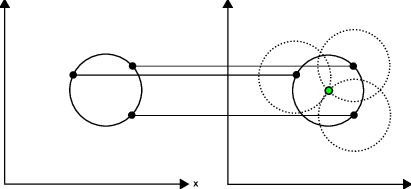
\includegraphics[width=\linewidth]{../Images/Design-Implementation/circle-hough-2d.png}\\
      {(a) Hough space for known radius \URI{https://www.researchgate.net/figure/The-circular-Hough-transform_fig1_242103081}}
    \end{minipage}%
    % -----------------
    \begin{minipage}{.5\textwidth}
      \centering
      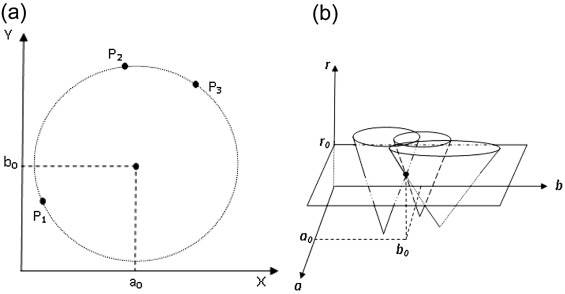
\includegraphics[width=.9\linewidth]{../Images/Design-Implementation/circle-hough-3d.jpg}\\
      {(b) Hough space for unknown radius \URI{https://www.sciencedirect.com/science/article/abs/pii/S0030402616316175}}
	\end{minipage}
	% -----------------
    \hfill \break
    \decoRule
    \CaptionBasedwithURL{Circle Hough Transform} 
    \label{fig:hough-tranform-examples}
\end{figure}

Η πιο σύνθετη περίπτωση - \Fig{hough-tranform-examples} (b) - είναι όταν δεν γνωρίζουμε την ακτίνα του κύκλου που αναζητούμε στην σκηνή, σε αυτήν την περίπτωση επαναλαμβάνουμε την παραπάνω διαδικασία για διαφορετικές τιμές ακτίνων, με αποτέλεσμα στο Hough space να δημιουργήσουμε κώνους αντί για κύκλους. Ενώ, οι συντεταγμένες του σημείου με τα περισσότερα votes στον accumulator, σε αυτήν την περίπτωση μας προσδιορίζουν τις συντεταγμένες του κέντρου του κύκλου μαζί με την ακτίνα του.

\subsubsection{Εναλλακτικές προσεγγίσεις}
Υπάρχουν αρκετές εναλλακτικές μεθοδολογίες που θα μπορούσαν επίσης να χρησιμοποιηθούν για το localization του object στο image plane, όπως το background extraction, tracking ενός object που γίνεται defined στην αρχή της λειτουργίας ή ακόμα και machine learning based προσεγγίσεις. 

Ένας επιπλέον, σύμφωνα με αυτά, τρόπος που έγινε προσπάθεια να εντοπιστεί - δυ\-στυ\-χώς χωρίς θετικά αποτελέσματα - η μπάλα στην εικόνα, είναι μέσω της τεχνικής haar cascade classifier \cite{opencv-haar-cascade} η οποία αποτελεί μία weak machine learning τακτική, που έχει χρησιμοποιηθεί στο παρελθόν σε ανίχνευση της μπάλας σε εφαρμογές όπως για RoboCup \cite{opencv-haar-cascade-robot1} \cite{opencv-haar-cascade-robot2}.

Πρακτικά, σε αυτή χρησιμοποιούνται δύο dataset, ένα θετικό στο οποίο παρουσιάζεται το αντικείμενο ενδιαφέροντος που θέλουμε να εκπαιδεύσουμε το μοντέλο να αναγνωρίζει και ένα αρνητικό στο οποίο δεν βρίσκεται. Για αυτόν τον λόγο, στην προσπάθεια να δημιουργηθεί ένα παρόμοιο μοντέλο για την συγκεκριμένη εφαρμογή πάρθηκαν πάνω από 1000 φωτογραφίες της μπάλας όπως παρουσιάζονται στην \Fig{haar-cascade-dataset-example} ενώ επίσης υπήρξαν και περίπου 4000 φωτογραφίες για το αρνητικό dataset.

\FigCaptLabelBasedURL{../Images/Design-Implementation/haar-cascade-clas-input-sample.jpg} %
{Παράδειγμα από το θετικό dataset που δημιουργήθηκε, για να γίνει train το μοντέλο του haar cascade.} %
{haar-cascade-dataset-example} %
<0.8>

% ------------------

\subsection{Εκτίμηση απόστασης}
Αφού είχε εντοπιστεί η θέση του αντικείμενο στην εικόνα καθώς και η ακτίνα του σε pixel μπορούσε να υπολογιστεί και η απόσταση του. 
Στον υπολογισμό της απόστασης της μπάλας από την κάμερα, χρησιμοποιείται ως κύρια αρχή ο φορμαλισμός που περιγράφηκε στη \Sect{theo-structure-from-reference} - \Equa{distance-from-object} - η οποία χρειάζεται να μετασχηματιστεί ώστε σαν είσοδο να χρησιμοποιεί πλήθος pixel και όχι mm, συνεπώς μέσω της εξίσωσης \EqNum{distance-from-object-pixels} μπορούμε να υπολογίσουμε την απόσταση της μπάλας από την κάμερα υπολογίζοντας μόνο το πλήθος των pixel που καταλαμβάνει στην εικόνα \cite{calculate-distance-stackexchange} \cite{calculate-distance-or-size-of-an-objectin-a-photo-image}.

\begin{align}
	\textrm{Distance (m)} &= \frac{\textrm{$f$ (mm)}\; x\;\textrm{Object's real size(m)}\; x\; \textrm{Image size(pixels)}}{\textrm{Object's size on sensor (pixels)}\; x\; \textrm{Sensor's size(mm)}} \label{eq:distance-from-object-pixels}
\end{align}

% ------------------

\subsection{Εκτίμηση γωνίας}
Για την εκτίμηση γωνίας ως προς τον x και y άξονα σε μία calibrated κάμερα μπορεί να χρησιμοποιηθεί η \Equa{angle-from-object-center-pixels}, η οποία είναι στην πραγματικότητα υλοποίηση απλής μέθοδος των τριών με βάση το Field of View (\Abbr{FOV}) μίας κάμερας. Σε περίπτωση που δεν γνωρίζουμε το \Abbr{FOV} μπορεί να υπολογιστεί με βάση την συσχέτιση του Angular Field of View (\Abbr{AFOV}) με το Focal length
της κάμερας, αυτή η εξάρτηση παρουσιάζεται οπτικά στην \Fig{focal-length-fov} και μαθηματικά στην \Equa{afov-focal-length} \cite{afov-focal-length-rela} και στην συνέχεια μέσω της σχέσης \EqNum{afov-to-fov} μπορούμε να μεταβούμε από το ένα στο άλλο. 

\begin{align}
	\textrm{Angle (\si{\degree})} &= \frac{\textrm{FOV(\si{\degree})}\; x\;\textrm{distance from origin (pixel)}}{\textrm{image length(pixel)}} \label{eq:angle-from-object-center-pixels}
\end{align}

\begin{align}
	\textrm{AFOV(\si{\radian})} &= 2\tan^{-1}{\frac{\textrm{image length(mm)}}{2\; x\;\textrm{focal length(mm)}}} \label{eq:afov-focal-length}
\end{align}

\begin{align}
	\textrm{FOV(\si{\degree})} &= \frac{\textrm{AFOV(\si{\radian})}\; x\;\textrm{180}}{\pi} \label{eq:afov-to-fov}
\end{align}

\FigCaptLabelBasedURL{../Images/Design-Implementation/fov-focal-length.png} %
{Συσχέτιση AFOV με focal length} %
{focal-length-fov} %
<0.7>
(https://www.princetoninstruments.com/learn/camera-fundamentals/field-of-view-and-angular-field-of-view)

%----------------------------------------------------------------------
\section{Διαμοιρασμός μηνυμάτων}
Προκειμένου να περαστεί πληροφορία μέσα στο δίκτυο με node, χρειάστηκε να δημιουργηθούν proprietary πακέτα, στα οποία θα αποθηκεύονταν χρήσιμη πληροφορία. Συγκεκριμένα κάθε node αφού πραγματοποιήσει όλη την επεξεργασία, αποστέλλει mocap\_worker\_data πακέτα, αυτά ακολουθούν την δομή που εμφανίζονται στην \Fig{proprietary-msg}, η οποία δημιουργήθηκε για τις ανάγκες του συστήματός και μέσα σε αυτή περιλαμβάνουν πληροφορίες, σχετικά με τον σειριακό αριθμό του node, την θέση του, τα χαρακτηριστικά της κάμερας του καθώς και πληροφορία για κάθε ανιχνευμένο αντικείμενο. 

% mocap_worker_data
% ├── timestamp
% ├── nodeID
% ├── master_time
% │   ├── ros_time
% │   ├── internal_time
% │   └── packet_id
% ├── obj_pose
% │   ├── x
% │   ├── y
% │   ├── z
% │   ├── roll
% │   ├── pitch
% │   └── yaw
% ├── camera_params
% │   ├── objectsRealSizeInMeter
% │   ├── imageHeightInPixels
% │   ├── imageWidthInPixels
% │   ├── XFieldOfViewInAngles
% │   ├── YFieldOfViewInAngles                    
% │   ├── XfocalLengthInMillimeters
% │   ├── YfocalLengthInMillimeters
% │   ├── XsensorSizeInMillimeters
% │   └── YsensorSizeInMillimeters
% └── detected_ball_data[]
%     ├── id
%     ├── color
%     ├── distance_from_camera
%     ├── image_plane_r
%     ├── image_plane_x
%     ├── image_plane_y
%     ├── xangle
%     └── ynagle
\FigCaptLabelBasedURL{../Images/Design-Implementation/ros-msgs-hier.png} %
{Η δομή του μηνύματος που αποστέλει κάθε node} %{Proprietary message send structure} %
{proprietary-msg} %
<0.4>

%----------------------------------------------------------------------
\section{Εντοπισμός θέσης αντικειμένου}\label{sec:implementation-obj-mult}
Για να εντοπιστεί τελικά στον τρισδιάστατο χώρο το αντικείμενο, χρησιμοποιείται η αρχή λειτουργίας του trilateration αλγορίθμου, που αναφέρθηκε στη \Sect{trilateration}. Που όμως επειδή είναι στον \Abbr{3D} χώρο, στον οποίο χρειαζόμαστε τουλάχιστον 4 κόμβους για τον καθορισμό της θέσης, ονομάζεται multilateration \ref{sec:Multilateration}. Όπως αναφέρθηκε και στη \Sect{trilateration}, πρακτικά προσπαθούμε για τις εξισώσεις \EqNum{multilateration-pha1} με γνωστά τα $(x_i, y_i, z_i)$ και $r_i$ να βρούμε τα $(x,y,z)$. 
 
\begin{align}
	(x-x_1)^2 + (y-y_1)^2 + (z-z_1)^2 &= r_1^2 \label{eq:multilateration-pha1} \\ 
	(x-x_2)^2 + (y-y_2)^2 + (z-z_2)^2 &= r_2^2 \nonumber \\
	(x-x_3)^2 + (y-y_3)^2 + (z-z_3)^2 &= r_3^2 \nonumber \\
	(x-x_4)^2 + (y-y_4)^2 + (z-z_4)^2 &= r_4^2 \nonumber 
\end{align}

Ένας τρόπος προσέγγισης, για επίλυση των εξισώσεων \EqNum{multilateration-pha1} είναι να τις αναλύσουμε στις \EqNum{multilateration-pha2} 
και από εκεί να έχουμε να λύσουμε το γραμμικό σύστημα πινάκων που περιγράγεται στην \EqNum{multilateration-linear-system}.

\begin{align}
	(x^2+y^2+z^2) - 2x_1x - 2y_1y - 2z_1z &= r_1^2 - x_1^2 - y_1^2 - z_1^2 \label{eq:multilateration-pha2} \\ 
	(x^2+y^2+z^2) - 2x_2x - 2y_2y - 2z_2z &= r_2^2 - x_2^2 - y_2^2 - z_2^2 \nonumber \\
	(x^2+y^2+z^2) - 2x_3x - 2y_3y - 2z_3z &= r_3^2 - x_3^2 - y_3^2 - z_3^2 \nonumber \\
	(x^2+y^2+z^2) - 2x_4x - 2y_4y - 2z_4z &= r_4^2 - x_4^2 - y_4^2 - z_4^2 \nonumber
\end{align}


\begin{align}
	A = \begin{bmatrix} 1 && -2x_1 && -2y_1 && -2z_1 \\ 1 && -2x_2 && -2y_2 && -2z_2 \\ 1 && -2x_3 && -2y_3 && -2z_3 \\ 1 && -2x_4 && -2y_4 && -2z_4 \\\end{bmatrix} \nonumber \quad
	X = \begin{bmatrix} x^2+y^2+z^2 \\x \\ y \\ z \end{bmatrix} \nonumber \quad
	B = \begin{bmatrix} r_1^2 - x_1^2 - y_1^2 - z_1^2 \\ r_2^2 - x_2^2 - y_2^2 - z_2^2 \\ r_3^2 - x_3^2 - y_3^2 - z_3^2 \\ r_4^2 - x_4^2 - y_4^2 - z_4^2 \end{bmatrix} \nonumber
\end{align}

\begin{align}
	AX = B \label{eq:multilateration-linear-system}
\end{align}

Θετικό με την συγκεκριμένη μέθοδο προσέγγισης - μέσω των εξισώσεων \EqNum{multilateration-pha2} - είναι ότι εύκολα το σύστημα μπορεί να γίνει scale καθώς η κάθε στήλη των πινάκων εξαρτάται μόνο από δεδομένα ενός μεμονωμένου node. Άρα παρόλο που στην συγκεκριμένη διπλωματική κάνουμε πειράματα για δεδομένα τεσσάρων θέσεων, με την ίδια ευκολία θα μπορούμε να ήταν και για N όπου $N>4$.

%----------------------------------------------------------------------
\section{Τρισδιάστατη απεικόνιση}
Για την τρισδιάστατη απεικόνιση των δεδομένων που συλλέχθηκαν κατά την διάρκεια των πειραμάτων - που περιγράφονται στο επόμενο κεφάλαιο - χρησιμοποιήθηκε το εργαλείο MATLAB, μέσω του οποίου έγιναν οι περισσότερες γραφικές. Σημαντική όμως είναι και η βοήθεια του πακέτου RViz του ROS, το οποίο σε real time χρόνο μπορεί να οπτικοποιήσει δεδομένα.

%----------------------------------------------------------------------

   % Design Features and Implementation
\chapter{FPGA Implementation} % Main chapter title
\label{Chapter5}
%\epigraph{The key to artificial intelligence has always been the representation.” }{\textit{Jeff Hawkins}}

\section{Tools Used}
The CNN (Inference) Hardware Accelerator was implemented using the Xilinx Vivado Design Suite - HL System Edition 2017.1. Vivado Design Suite is a software suite developed by Xilinx for synthesis and analysis of HDL designs, superseding Xilinx ISE with additional features for system on a chip development and high-level synthesis. The tools used are the Vivado HLS, Vivado IDE, and Xilinx SDK \cite{Link1}.

\subsection{Vivado HLS}
The Xilinx Vivado HLS tool \cite{Link3} provides a higher level of abstraction for the user by synthesizing functions written in C,C++ (with constraints and feautures) into IP blocks, by generating the appropriate ,low-level, VHDL and Verilog code. Then those blocks can be integrated into a real hardware system. Vivado HLS is tightly integrated with the rest of the Xilinx design tools and provides comprehensive language support and features for lower level optimizations, making it possible to optimize the C code for hardware systems.
The Vivado HLS tool allows for C functions written in C, C++, SystemC, or an OpenCL API C kernel. We decided to use C++, as there are several supported features in HLS design (template e.t.c.) . To debug the code, Vivado HLS uses a C test bench to simulate the C function prior to synthesis and to verify the RTL output using C/RTL Cosimulation.

The tool also adds some constraints to the exported IP block, like the clock period, clock uncertainty, and FPGA target. The clock uncertainty defaults to 12.5\% of the clock period, but you have the option to change it. Finally, the tool allows for directives to be added to direct the synthesis process to implement a specific behavior or optimization. Directives are optional and do not change the behavior of the c code in the simulations, only in the synthesized IP block.  

\subsubsection{Synthesis Report in Vivado HLS}

When synthesize an HLS code tool exports a synthesis report showing the performance metrics of the generated design. The report's information on performance metrics are presented below:
\begin{itemize}
  \item \textbf{Area:} Amount of hardware resources required to implement the design based on the resources available in the target FPGA. The types of resources are, Look-Up Tables (LUT), Flip Flops (FF) , Block RAMs (BRAMs), and DSP48s.
  \item \textbf{Latency:} Number of clock cycles required for the function to compute all output values.
  \item \textbf{Iteration Interval (II):} Number of clock cycles before the function can accept new input data.
  \item \textbf{Loop Initiation Interval:} Number of clock cycle before the next iteration of the loop starts to process data.
   \item \textbf{Loop Latency:} Number of cycles to execute all iterations of the loop.
  \item \textbf{Loop Iteration Latency:} Number of clock cycles it takes to complete one iteration of the loop.
\end{itemize}


\subsubsection{Optimizations in Vivado HLS}
 Vivado HLS also provides (optional) directives that can be used to optimize the design: reduce latency, improve throughput performance, and reduce area and device resource utilization of the resulting RTL code. These pragmas can be added directly to th1e source code for the kernel.  
\begin{itemize}

    \item \textbf{Pipeline}: The PIPELINE pragma reduces the initiation interval for a function or loop by allowing the concurrent execution of operations. A pipelined function or loop can process new inputs every N clock cycles, where N is the initiation interval (II) of the loop or function. 
    
    \item \textbf{Array Partition}: Partitions an array into smaller arrays or individual elements.
    
This partitioning:
\begin{itemize}
    \item Results in RTL with multiple small memories or multiple registers instead of one large memory.
    \item Effectively increases the amount of read and write ports for the storage.
    \item Potentially improves the throughput of the design.
    Requires more memory instances or registers.
\end{itemize}

    
    \item \textbf{Unroll}: Unroll loops to create multiple independent operations rather than a single collection of operations. The UNROLL pragma transforms loops by creating multiples copies of the loop body in the RTL design, which allows some or all loop iterations to occur in parallel. 
 
    \item \textbf{Stream}:By default, array variables are implemented as RAM. If the data stored in the array is consumed or produced in a sequential manner, a more efficient communication mechanism is to use streaming data as specified by the STREAM pragma, where FIFOs are used instead of RAMs.

    \item \textbf{Array Map}: Combines multiple smaller arrays into a single large array to help reduce block RAM resources.

    \item \textbf{Resource}: Specify that a specific library resource (core) is used to implement a variable (array, arithmetic operation or function argument) in the RTL. If the RESOURCE pragma is not specified, Vivado HLS determines the resource to use.    

    \item \textbf{Dataflow}: The DATAFLOW pragma enables task-level pipelining, allowing functions and loops to overlap in their operation, increasing the concurrency of the RTL implementation, and increasing the overall throughput of the design.\newline \newline
    
    
\end{itemize}



\subsection{Vivado IDE}

The Vivado IDE ( was implemented from  co-partner Giannis Kalomoiris) is the GUI for the Vivado Design Suite. All of the Vivado design Suite tools are written with a native Tcl interface, and all of those commands are available through the IDE either through the GUI or through the Tcl console. Tcl commands can be entered in the Tcl Console in the Vivado IDE or using the Vivado Design Suite Tcl shell. You can run analysis and assign constraints throughout the design process. Timing and power estimations are provided after synthesis, placement, and routing. 
 



\subsection{Vivado SDK}

The Xilinx SDK is an IDE tool to develop embedded software applications targeted towards Xilinx ARM processors. The SDK works with hardware designs and bitstreams created with Vivado Design Suite. The SDK is based on the Eclipse standard. SDK includes an  C/C++ code editor and a compilation environment with easy project management, application build configuration and automatic Makefile generation. It also provides an environment for debugging and profiling of software code as well as design performance. The SDK also provides it own tools to configure FPGAs and create bootable bitstrems with software extensions.
We open the SDK (through IDE) using the preconfigured directories, including bitsreams after successful Vivado IDE implementation. The SDK automatically imports the project hardware wrapper and generates the files needed(memory porting , defines ,etc) for the software part. Therefore we create a new fuzzy project which generates the project files,and the needed BSP packages, which includes the suitable drivers for the software design that the PS has access to.

The SDK is fisrtsly used to create a simple program to run by the PS to test and debug the PL functionality. To be able to program the FPGA, the JTAG port has to be connected to the PC, and to monitor and debug it we use the UART port as well. Another very useful tool that is part of the Vivado IDE is the Hardware Manager. It connects to the ILAs that have been added to the Vivado project and allows us to monitor in real-time the values of the signals between our modules, while the program is running.

For the needs of the SDK, we have created functions where activate and initialize our IPs, DMA, memories, and caches. Additionally, functions for writing and reading data from the SD card were implemented. We made a study to be able to measure the real memory bandwidth. The data was stored in the DDR in 2 ways either by SD read or JTAG. Finally, time measurement functions were used to enable speedups to be evaluated.




\section{FPGA platforms}

Our architectures are targetting on 2 FPGA platforms we worked on.
\subsection{Xilinx Zynq UltraScale+ MPSoC ZCU102}

The ZCU102 is a general purpose evaluation board for rapid-prototyping based on the Zynq UltraScale+ XCZU9EG-2FFVB1156E-2-i MPSoC (multiprocessor system-on-chip). High-speed DDR4 SODIMM and component memory interfaces, FMC expansion ports, multi-gigabit per second serial transceivers, a variety of peripheral interfaces, and FPGA logic for user customized designs provides a flexible prototyping platform.

Below in table \ref{tab:7} we present main features of the FPGA


\begin{table}[h]
\captionof{table}{ZCU102 Specifications} \label{tab:7} 
\centering
\begin{tabular}{l l l l l l}
\toprule
\tabhead{Logic Cells} & \tabhead{B-RAM} & \tabhead{DSP Slices} & \tabhead{PS DDR} & \tabhead{PL DDR} \\
\tabhead{(K)} & \tabhead{(MB)} & \tabhead{} & \tabhead{(GB)} & \tabhead{(MB)} \\
\midrule

600 & 4  & 25200 & 4 & 512\\

\bottomrule
\end{tabular}\par
\end{table}
\begin{center}
MB=Mbytes , GB=Gbytes
\end{center}


\subsection{QFDB}
QFDB is a 4-FPGA custom platform designed and implemented by FORTH. It has 4 ZCU102 FPGA,(meaning 4x powerful than ZCU102) thus our architecture transference between platforms are fully compatible. 

\section{Bottom-up Strategy}
The first approach was implemented with the bottom-up strategy. A bottom-up approach is the unification of many "simple" systems to end up in a more "complex" system.



%%%%%%%% /////////////eikona


The algorithm was divided into small entities with specific behavior and hierarchical structure. Then they would be joined together to make the overall accelerator. The entities were separated as follows:
\begin{itemize}

    \item \textbf{Convolution (1-D) }(conv1): $1^{st}$ Convolutional layer of the network (Input: image, kernel1, bias1)(Output:ConvStage1)
    \item \textbf{Convolution (2-D) }(conv2): $2^{nd}$ Convolutional layer of the network (Input: ConvStage1, kernel2, bias2)(Output:ConvStage2)
    \item \textbf{Convolution (2-D) }(conv3): $3^{rd}$ Convolutional layer of the network (Input: ConvStage2, kernel3, bias3)(Output:ConvStage3)
    \item \textbf{Fully Connected }(fc):  Fully Connected of the network (Input: ConvStage3, $kernel_{dense}$, $bias_{dense}$)(Output:Classification) 

    \item \textbf{ReLU} : ReLU is the main activation function that was performed after every convolutional layer. For this purpose, ReLU was inserted in every Convolutional Layer entity.
\end{itemize}


\subsection{Two Stage Architecture}
After the network was divided and depicted in small entities, they were reunited to make the two basic modules of our architecture. The first module is  "Convolutional Layers" where it contains the three Convolutional Layer with the corresponding ReLU. The second module is the "Fully Connected Layer" where it receives the exit of the first module and makes the final classification.
This leads to a 2-Stage Architecture designed to communicate 2 FPGAs. The first will implement Convolution and the second the Fully Connected module \ref{fig:21}.

\begin{figure}[h]
\centering
\includegraphics[width=\textwidth]{Images/datapath_2Stage.png} 
\decoRule
\caption[Datapath of Two-Stage Architecture]{Datapath of Two-Stage Architecture
}
\label{fig:21}
\end{figure}

\section{First Approach}

\subsection{Memory and I/0}
Firstly we have to clarify how to insert the data into the different Building Blocks of the accelerator from the outside world. The first step is to pass the data to the DDR of the processor. Then we have three ways to link this data to FPGA:
\begin{itemize}

    \item \textbf{Memory-mapped I/O }(MMIO): A complementary method of performing input/output (I/O) between the central processing unit (CPU) and peripheral devices such as FPGA. This method uses the same address space to address both memory and I/O extensions. The memory and registers of the I/O devices are mapped to (associated with) address values. This technique comes to emphasize the main DDR drawback, which is that it can not efficiently drive multiple requests because it is random access. This means that for each request we would have to "pay" the initial interval (30 -50 cycles) and so there would be no meaning for pipeline design in the FPGA. This technique can be implemented through using Xilinx's IP Data-movers.
    
    \item \textbf{Streaming }(AXI-4): The second method we can use is Streaming Interface using AXI-4 protocol. In fact, we are creating a continuous DDR communication channel with FPGA (a large FIFO) and we are sending the processor the data we want without requests. This relieves us from the delay of requests, and you create a huge pipeline for entering data by hiding the DDR interval. This technique can be implemented through using Xilinx's IP DMA. 
    
    \item \textbf{B-RAM }: Another approach is to transfer the data in burst with memory mapped or stream and then store them in B-RAM to take advantage of the huge bandwidth. In order to achieve this, the data must have a small memory footprint. Typically the B-RAM is in the order of many KBs and a few MBs. \newline \newline
    
    
\end{itemize}

Using Streaming Interface is much more efficient because it allows us to fully utilize the DDR bandwidth (about 10 GBs). However, this method can be used only in cases where we know in advance the data-flow. CNNs have inherently streaming nature, so they are ideal for taking advantage of this.

\subsection{Transference to HLS}

A next step was to be able to integrate each Entity's algorithm parts from MATLAB into C++ and then into HLS synthesizable code. In order to successfully complete this, the limitations and capabilities of the tool had to be studied. Convolution was the most algorithmic complex part. On the other hand, Matrix Multiplication has less algorithmic complexity, but it requires much more computation time.

\subsection {Convolution (1-D)}
First, we grant the weights and the image into the FPGA and store them in the internal B-RAM. This approach came because we need to use that data several times. The reasoning in the use of B-RAM instead of sending the data with Stream interface was to be able to exploit its bandwidth (TBs).

\begin{figure}[h]
\centering
\includegraphics[width=\textwidth]{Images/Convolution1_Datapath.png} 
\decoRule
\caption[Datapath of Convolution(1-D)]{Datapath of Convolution(1-D)}
\label{fig:22}
\end{figure}


\subsubsection{Array Partitioning}
B-RAM has memory access limitations because it has two memory channels. A feature that HLS provides you is the option to partition a B-RAM array. This allows you to have more than two memory accesses in a clock cycle. Essentially it creates copies of your original array with the use of multiplexer systems. The nature of the algorithm is access to specific arrays many times in the same cycle, so it is advisable to use this directive.

\subsubsection{Pipeline}
In FPGA designing, it is very important to manage running your algorithm in a large pipeline, thus taking advantage of FPGA's capabilities. However, in order to succeed Pipeline, a limitation that came up was algorithmic. We basically wanted to process an 8-part set, e.g. 0-7, of the image in a cycle. In the next cycle, we have to retain the last 7 parts and store the next part, having at the end of this cycle a new 8-part set e.g. 1-8 (stride=1 of the network). This was approached by creating a new dimension in the image and implementing it as a shifted B-RAM, achieving by that pipeline=1.

%%%%%%%%%%%%%sxima 1-7 2-8
%%%%%%%%%%%%%
\subsection {Convolution (2-D)}

The complexity of this entity is 16x compared to Convolution(1-D), as it has an extra dimension size of 16. The weights and the image are granted into the FPGA and store them in the internal B-RAM with the same way. This approach came because we need to use that data several times. The reasoning in the use of B-RAM instead of sending the data with Stream interface was to be able to exploit its bandwidth (TBs).

\subsubsection{Array Partitioning}
B-RAM has memory access limitations because it has two memory channels. A feature that HLS provides you is the option to partition a B-RAM array. This allows you to have more than two memory accesses in a clock cycle. Essentially it creates copies of your original array with the use of multiplexer systems. The nature of the algorithm is access to specific arrays many times in the same cycle, so it is advisable to use this directive.

\subsubsection{Pipeline}
In order to succeed Pipeline a limitation that came up was also algorithmic. We basically wanted to process 16x8 parts of the image in a cycle and in the next cycle to retain the last 16x7 and store the next 16 part (stride=1 of the network). This was approached by creating a new dimension in the image and implementing it as a shifted B-RAM, achieving by that an overall pipeline=8.The time-chart of Convolutional Layers presents in figure \ref{fig:conv_simple}.

 \begin{figure}[h]
\centering
\includegraphics[width=\textwidth]{Images/Conv_simple.png} 
\decoRule
\caption[Convolutional Layers Time-Chart (FA)]{Convolutional Layers Time-Chart of First Approach}
\label{fig:conv_simple}
\end{figure}

\subsection {Fully Connected}
The idea of the streaming interface was fully utilized to implement Fully Connected Layer. We store into B-RAM the least possible data(image stage, bias) and we basically stream the weights from DDR. The reason for this is because weights of the dense layers could not be stored into B-RAM. \ref{fig:fc_mod}

\begin{figure}[h]
\centering
\includegraphics[width=\textwidth]{Images/Fully_Connect.png} 
\decoRule
\caption[Fully Connected Module]{Fully Connected Module}
\label{fig:fc_mod}
\end{figure}

\subsubsection{Pipeline}
A Pipeline (Iteration Interval=1) has been implemented essentially by export each partial result in each cycle. The time-chart of CNN presents in figure \ref{fig:cnn_simple}.


\begin{table}[h]
\caption{First Approach Performance}
\label{tab:1}
\centering
\begin{tabular}{l l l l}
\toprule
\tabhead{Modules} & \tabhead{Latency} & \tabhead{Comp. Performance} &\tabhead{Bandwidth} \\
\tabhead{} & \tabhead{(cycles)} & \tabhead{(GFLOPS)} &\tabhead{(GB/s)} \\
\\
\midrule
conv & 593596 & 7.6   & 1\\
dense & 22971200  & 0.6   & 1\\
conv+dense & 23564796  & 0.77  & 1\\
\bottomrule
\end{tabular}
\end{table}

\begin{center}
GB=Gbytes
\end{center}

In computing, floating point operations per second (FLOPS, flops or flop/s) is an important measure of computational performance, useful in fields of scientific computations that require floating-point calculations \ref{eq:FLOPs}.

\begin{equation}\label{eq:FLOPs}
FLOPS=\frac{cycles}{second}*\frac{FLOPs}{cycle}
\end{equation}


 \begin{figure}[h]
\centering
\includegraphics[width=\textwidth]{Images/FCNN_simple.png} 
\decoRule
\caption[CNN Time-Chart (FA)]{CNN Time-Chart of First Approach}
\label{fig:cnn_simple}
\end{figure}

\section{A better Approach}
After the first approach was realized how long we were from a possible speedup over the GPU. The main obstacle was that we did not use the maximum DDR Bandwidth (we used 1GB / s, meaning 6\% of the maximum theoretical Bandwidth), resulting in the failure to exploit the processing power of the FPGA.

\subsection{Larger Streaming Buses}
The next action is to try to limit ourselves from the bandwidth of DDR. Consequently, we tried to use larger memory streaming buses (more than 32bits). The limitations here are three:

\begin{itemize}

    \item \textbf{DMA}: The maximum memory bus that DMA can support is 1024 Bits in one cycle.
     
     \item \textbf{DDR Bandwidth}: The maximum bandwidth of the DDR is 16GB/s. So the maximum bus considering 300MHz clock we can support is 458 bit from \ref{eq:8}.
    \item \textbf{HP ports }: The maximum memory bus that the CPU can transfer from memory to FPGA through DMA. This is done through HP ports and the limit is 128-bit. \newline \newline
    
\end{itemize}

\begin{equation}\label{eq:8}
  Bus_{BitWidth}= \frac{Bandwidth}{Clock_{frequency}}
  \end{equation}
  \begin{center}
       \small{Bandwidth=Memory Bandwidth in b/s , $Clock_{frequency}$ of the FPGA} \newline 
  \end{center}

Therefore we end up using 128 bits, that is 4 times larger than the previous ones. This means we use 4 times more memory bandwidth. This could lead to a 4x speedup by implementing the ideal architecture. 

\subsection{Multiple DMAs}
Next, we realize that even though we used 4GB/s bandwidth we have not reached its full potential(16GB/s). The next solution we can exploit is to use multiple DMAs where they will stream from different HP ports (maximum 6) data linking in the same DDR. Theoretically, 4 DMAs is the golden ratio because we will be totally restrained from the memory. 

\subsubsection{DDR Bandwidth}
In order to be convinced how many DMAs (and HP ports) would be the best to use we did some fuzzy IPs (which reads and writes random values through DMAs) to be able to accurately count read, write and read/write bandwidth as showing table \ref{tab:8}. Furthermore to achieve higher bandwidth we enabled caches and flushed them with the weights.

\begin{table}[h]
\captionof{table}{Memory Bandwidth} \label{tab:8} 
\centering
\begin{tabular}{l l l l l }
\toprule
\tabhead{HP ports} & \tabhead{Read BW} & \tabhead{Write BW} & \tabhead{Read/Write BW}  \\
\tabhead{} & \tabhead{(GB/s)} & \tabhead{(GB/s)} & \tabhead{(GB/s)}  \\

\midrule

1 & 4.15  & 4.15 & 4.18  \\
2 & 8.24  & 8.23 & 8.3  \\
3 & 9.8  & 9.9 & 12.4 \\
4 & 10.2  & 10.4 & 16.8 \\
\bottomrule
\end{tabular}\par
\begin{center}
GB=Gbytes
\end{center}
\end{table}



Read and Write channels are separated, so it makes sense not to see a linear increase in bandwidth for reading and write separately. Whereas when we use both channels we see linearity.
Our algorithm is using the read channel much more because it requires to read more data than to write in the final classification. Therefore we conclude that the best possible case for not consuming resources is to use 2 HP ports and 2 DMAs.


\subsection {Convolution (1-D) and Convolution (2-D)}

Having 8 times higher bandwidth than the first approach we can store B-RAM 8 times faster. The rest and most of the implementation reads the data through B-RAM, so there is no significant optimization.



\subsection {Fully Connected}

On the other hand, the fully connected was clearly set up as streaming oriented IP. Now by bringing 8 times more data (2 DMA (128) -> 256 bit versus 32bit), we must take advantage of this feature and come up with  8x speedup relation to the first approach.

\paragraph {Multiply and Accumulate}
To be able to achieve this we need to observe from a different perspective the basic operation of multiply and accumulate and try to "hide" the Latency of the 10 cycles it needs. In order to be able to exploit the rate that weights are being streamed in, we have to increase the parallelism at the level of operations.

\paragraph{First Approach} Trying to make the 8-fold multiplication and addition based on the current Fully Connected implementation end up in a Pipeline equal to the accumulative delay (10 in our case), something that does not satisfy us \ref{alg:MAC_1}. This leads to a very poor exploit of the memory bandwidth. It is perceptible that we have to follow a different implementation trying to achieve a full pipeline module, managing to hide the MAC operation delay.


\begin{algorithm}[h]
\caption{Matrix Multiplication}\label{alg:MAC_1}
\begin{algorithmic}[1]
\Procedure{Matrix Multiplication}{$input,weights$}  
\State $NumOfClasses \gets size(weights,1)$ \Comment{Number of Classes}
\State $NumOfWeights \gets size(weights,2)$ \Comment{Number of Weights/Class}
 \State $FaddLat=10$ \Comment{Latency of Multiply and Accumulate}
\For{i:=1 \textbf{to} NumOfClasses }     
\State $Classes(i)\gets 0$
\EndFor 
 \State $sum\gets 0$

\For{i:=1 \textbf{to} NumOfClasses }

\State $sum=0$
\For{j:=1 \textbf{to} NumOfWeights }           
\State $ PIPELINE=FaddLat$
\State $sum \gets sum + input(j)*weights(i,j)$
\EndFor 
\State $Classes(i)\gets sum$
\EndFor 

\State \textbf{return} $Classes$       
\EndProcedure
\end{algorithmic}
\end{algorithm}

\paragraph {Better Approach}To achieve that we will perform the task in a different way. In fact, we will calculate different partial results in parallel for each class. We will end up having the partial results that need to be added to produce a result. This will be achieved by creating a deep adder tree. The appropriate number of different partial results must be equal to the adder delay, meaning 10 in \ref{alg:MAC_2}.

\paragraph {Cyclic Array}
We originally solved the problem of how we process the 8-fold weights in a single clock cycle and exploit the resources to do the 8-fold multiplication and addition. Instantly the problem that arises is to explore how we will ensure access to 8-Images stages of the edited image (in a cycle). This could easily be achieved using the array partition of the tool by applying a cyclic partition. This allows us, depending on the factor we will set, in how many consecutive cells of the array we will have access ( in a cycle). However, because the array was large (28464), the tool used a large multiplexer system to route access to the memory and thus did not allow us to reach a competent clock (it greatly increased the critical path).

\paragraph {Custom Cyclic Array}
So we ended up making our own "cyclic partition" helping the tool to achieve the behavior we wanted. To achieve this we created 4 subterranean arrays of the original one. We created 4 and not 8 because each B-RAM has 2 memory channels, meaning 2 memory accesses. We stored weight1,weight2 in the first table, weight3,weight4 in the second etc. in order to be able to have access in 8 consecutive image-stages. Hence we use a same sized B-RAM, but instead of reading from 1 array, we now read from 4 different subterranean arrays by striking the behavior we wanted. Finally, we ended up creating our own "cyclic partition" helping the tool to achieve the behavior we wanted.

\begin{algorithm}[h]
\caption{Matrix Multiplication (Opt)}\label{alg:MAC_2}
\begin{algorithmic}[1]
\Procedure{Matrix Multiplication}{$input,weights$}  
\State $NumOfClasses \gets size(weights,1)$ \Comment{Number of Classes}
\State $NumOfWeights \gets size(weights,2)$ \Comment{Number of Weights/Class}
\State $FaddLat=10$ \Comment{Latency of Multiply and Accumulate}

\For{i:=1 \textbf{to} NumOfClasses }     
\State $ UNROLL$
\State $Classes(i)\gets 0$
\EndFor 

\For{i:=1 \textbf{to} FaddLat}     
\State $ UNROLL$
\State $partialSum(i) \gets 0$
\EndFor 


\For{i:=1 \textbf{to} NumOfClasses \textbf{step}=FaddLat }
\State $ PIPELINE II=FaddLat$

\For{k:=1 \textbf{to} FaddLat }     
\State $ UNROLL$
\State $partialSum(k)\gets 0$
\EndFor 
\For{j:=1 \textbf{to} NumOfWeights }           

\State $partialSum(j) \gets partialSum(j) + input(j)*weights(i,j)$
\EndFor 

\For{v:=1 \textbf{to} FaddLat }     
\State $UNROLL$
\State $Classes(k)\gets Classes(k)+partialSum(v)$
\EndFor 

\EndFor 

\State \textbf{return} $Classes$       
\EndProcedure
\end{algorithmic}
\end{algorithm}



\begin{table}[h]
\caption{Second Approach Performance}
\label{tab:1}
\centering
\begin{tabular}{l l l l}
\toprule
\tabhead{Modules} & \tabhead{Latency} & \tabhead{Comp. Performance} &\tabhead{Bandwidth} \\
\tabhead{} & \tabhead{(cycles)} & \tabhead{(GFLOPS)} &\tabhead{(GB/s)} \\
\midrule
conv & 593596 & 7.6  & 1\\
dense & 2871400 & 4.8  & 8.23\\
conv+dense & 3464996 & 5.25  & 9.23\\
\bottomrule\\
\end{tabular}
\begin{center}
GB=Gbytes
\end{center}
\end{table}



\section{Architecture v1.0}
In this architecture, we basically integrate the study implemented in Sensitivity Analysis \ref{Chapter4}. We have been able to reduce the memory footprint of weights to a satisfactory degree with small error. Hence we can speed the processing of our data. Then we managed to make our network a huge pipeline from the image entering and communication of Convolution Layers to the communication of the three Convolutional Layers with the Fully Connected Layer. Afterwards, we perform resource optimizations to be able to fit our network into an FPGA.
 
 
 \begin{figure}[h]
\centering
\includegraphics[width=\textwidth]{Images/Datapath_Arch1.png} 
\decoRule
\caption[Datapath of the Architecture v1.0]{Datapath of the Architecture v1.0}
\label{fig:27}
\end{figure}

\subsection{Embedding Compressed Weights}
Originally, the analysis was done to reduce the memory footprint of the weights that only applies to the fully connected, because this is the main memory bottleneck of the algorithm. Furthermore, compressed weights are used in the I/O streaming interface during the processing. We used 256-bit channel from the memory (2-DMA of 128 bits) based on the previous analysis on memory buses. Each compressed weight has a 4-bit size. Therefore we can stream 64 weights in a cycle(stream read). This gives us a possibility for a huge parallelism at the operation level. To achieve this we extend the previous architecture to operation level parallelism.

\subsection{Pipelining Convolution Module}
The next step is to try to get the most out of all available resources. To accomplish this, a pipeline must be created between convolutional layers as shown in figure \ref{fig:conv_pipe}, in such a way that different parts of the image are processed at the same time by the three convolutional entities.


To perform this we need to change the way we obtain the data and output them to the next entity in a way that is suitable for it, to process them in parallel with the previous one. FIFO must be placed between the layers. Thus we create a channel in which every entity will be able to obtain image-parts. We need to introduce some new entities with specific behavior that will satisfy this purpose and will enable pipeline processing.


 \begin{figure}[h]
\centering
\includegraphics[width=\textwidth]{Images/Pipeline_Con.png} 
\decoRule
\caption[Convolutional Layers Time-Chart (Arch1.)]{Convolutional Layers Time-Chart of Architecture v1.0}
\label{fig:conv_pipe}
\end{figure}

In table \ref{tab:pipe_conv_arch1} we present performance results after the pipeline of Convolutional Layers.


\begin{table}[h]
\caption{Pipeline Convolutional Layers}
\label{tab:pipe_conv_arch1}
\centering
\begin{tabular}{l l l }
\toprule
\tabhead{Modules} & \tabhead{FLOPS} & \tabhead{MAC/cycle}   \\
\midrule
conv1 & 459K & 8 \\
conv2 & 7.3M & 16  \\
conv3 & 7.3M & 16 \\
CONV & 15.1M & 40(peak) \\
\bottomrule\\
\end{tabular}
\begin{center}
GB=Gbytes
MAC = Multiply and Accumulate
FLOPS = Floating Point Operations
\end{center}
\end{table}


\subsubsection{Shifted FIFO}

The utility of this entity is double. Originally, this implements a custom behavior of a Shifted FIFO. It receives data from the previous layer, and when it reaches 16x8 it pushes it in 16 packages and streams them through a FIFO (512 bits) to the next Layer to start the processing. Then in the next cycle, the next module will need the last 16x7 + the new 16 data. Therefore here comes the shift register. At the same time, we do not have to store some of the stages of the image (like before in B-RAM), we just go through FIFOs and read them there. The shift register functionality could be added to the next layer. However, this has led to great critical paths and that's why its behavior has taken place in a different entity.

\subsubsection{Task Level Parallelism}
Having created all the structures to activate the pipeline, the next step is to use the Xilinx dataflow pragma. However, trying to incorporate it, we realized that there was a feature, sequential and parallel processing in different modules at the same time, that was not supported. As a result, when the tool noticed any FIFO or some kind of stream behavior, it was trying to turn it into task level parallelism.

\paragraph{Sequential and Parallel Processing}

Accordingly, we should find a workaround to incorporate this feature. This problem was presented in the insertion of the initial data (image, weights, bias) in the 1st module. Essentially we were reading at several points from the same stream and stored in different B-RAMs. The solution was to create a custom mutual exclusion for reading in this stream (mutex). Therefore we forced the tool to read in a specific manner the information and store it in specific B-RAMs. On the other hand, the image is passed to an internal FIFO to continue the flow in the next modules.
Below in \ref{alg:SP} we present the behavior above.

\begin{algorithm}[h]
\caption{Sequential Parallel with MUTEX}\label{alg:SP}
\begin{algorithmic}[1]
\Procedure{Sequential Parallel with MUTEX}{$InStream$}  
\State $SKernel_{1} \gets size(kernel_{1})$ \Comment{Size of $kernel_{1}$}
\State $SKernel_{2} \gets size(kernel_{2})$ \Comment{Size of $kernel_{2}$}
\State $SKernel_{3} \gets size(kernel_{3})$ \Comment{Size of $kernel_{3}$}
\State $SBias_{1} \gets size(bias_{1})$ \Comment{Size of $bias_{1}$}
\State $SBias_{2} \gets size(bias_{2})$ \Comment{Size of $bias_{2}$}
\State $SBias_{3} \gets size(bias_{3})$ \Comment{Size of $bias_{3}$}
\State $SImage \gets size(Image)$ \Comment{Size of Image}
\State $TotalSize \gets SKernel_{1}+SKernel_{2}+SKernel_{3}+SBias_{1}*3$ \Comment{Total Size}

\For{i:=1 \textbf{to} TotalSize }     
\If{$i\leq SKernel_{1}$}
\State $Kernel_{1}(i) \gets InStream.read$ 
\ElsIf{$i\leq SKernel_{1}+SKernel_{2}$}
\State $k\gets i-SKernel_{1}$ 
\State $Kernel_{2}(k) \gets InStream.read$ 
\ElsIf{$i\leq SKernel_{1}+SKernel_{2}+SKernel_{3}$}
\State $k\gets i-SKernel_{1}+SKernel_{2}$ 
\State $Kernel_{3}(k) \gets InStream.read$ 
\ElsIf{$i\leq SKernel_{1}+SKernel_{2}+SKernel_{3}+SBias_{1}$}
\State $k\gets i-SKernel_{1}+SKernel_{2}+SKernel_{3}$ 
\State $Bias_{1}(k) \gets InStream.read$ 
\ElsIf{$i\leq SKernel_{1}+SKernel_{2}+SKernel_{3}+SBias_{1}*2$}
\State $k\gets i-SKernel_{1}+SKernel_{2}+SKernel_{3}+SBias_{1}$ 
\State $Bias_{2}(k) \gets InStream.read$ 
\ElsIf{$i\leq SKernel_{1}+SKernel_{2}+SKernel_{3}+SBias_{1}*3$}
\State $k\gets i-SKernel_{1}+SKernel_{2}+SKernel_{3}+SBias_{1}*2$ 
\State $Bias_{3}(k) \gets InStream.read$ 
\ElsIf{$i\leq TotalSize$}
\State $StreamImage.Write(InStream.read)$ 
\EndIf
\EndFor 

\State \textbf{return} $Kernel_{1},Kernel_{2},Kernel_{3},Bias_{1},Bias_{2},Bias_{3},StreamImage$       
\EndProcedure
\end{algorithmic}
\end{algorithm}


\subsection{Pipelining two Modules}
The next step is to be able to pipeline the two main modules of the Convolution Layers and Fully Connected networks, as shown in figure \ref{fig:cnn_pipe}. When we achieve this, we will essentially gain the latency of the smallest module in total latency \ref{eq:9}.

 \begin{figure}[h]
\centering
\includegraphics[width=\textwidth]{Images/FCNN_Pipe.png} 
\decoRule
\caption[CNN Time-Chart (Arch1)]{CNN Time-Chart of Architecture v1.0}
\label{fig:cnn_pipe}
\end{figure}
 
\begin{equation}   \label{eq:9}
{
Lat_{TOTAL}=max(Lat_{CONV},Lat_{FC}+LatencyInterval)
}
\end{equation}
 
To accomplish this, major modifications have to be made to the 2 modules.

\subsubsection{Convolution Transformations}
Convolution should transform the way we export the data. For these purposes, a new entity was created by FifoToPackedFifo. This entity gets the processed image and packs it into 32 items. That's why we would need a 1024bits FIFO. This feature is not supported by HLS, so we came with a workaround by having two 512 FIFOs each containing half of the data. After the initial latency interval, every 32 * 8 = 512 cycles, it feeds the Fully Connected Layer through FIFO.

\subsubsection{Fully Connected Transformations}
With regard to the Fully Connected Layer, the way the processed image is imported should be transformed according to the above changes. Next, we need to try to gain the most out of the data that comes, or else we can drive the system into huge stalls and thus destroy the Pipeline. The way the FC has so far operated was to calculate the results for each class individually. For each class, we had to read the whole processed image again. This cannot be continued because the whole processed image will be available only when the Conv module has finished its processing. This would mean the pipeline concept will be lost. Hence we have to change the way we calculate the classes. Another dimension of parallelism needs to be added. There has to be another important change in the structure of FC. We will create 2 FC Modules where each will calculate different classes. So in 400 cycles, we will have partial results for the 800 classes. To achieve this, we need to perform a Memory Layout Transformation where it will also transform the way that weights are streamed. 


\begin{algorithm}[h]
\caption{Matrix Multiplication (Opt)}\label{alg:MAC_3}
\begin{algorithmic}[1]
\Procedure{Matrix Multiplication}{$InStream,ConvStream,input,weights$}  
\State $NumOfClasses \gets size(weights,1)$ \Comment{Number of Classes}
\State $NumOfWeights \gets size(weights,2)$ \Comment{Number of Weights/Class}
\State $FaddLat=10$ \Comment{Latency of Multiply and Accumulate}

\For{i:=1 \textbf{to} NumOfClasses }     
\State $ UNROLL$
\State $Classes(i)\gets Dense_{bias}(i)$
\EndFor 

\For{i:=1 \textbf{to} FaddLat}     
\State $ UNROLL$
\State $partialSum(i) \gets 0$
\EndFor 



\For{i:=1 \textbf{to} NumOfWeights/32 }           

\State $ConvStream.read()$

\For{j:=1 \textbf{to} NumOfClasses \textbf{step}=FaddLat}           
PIPELINE=10
\For{k:=1 \textbf{to} FaddLat} 
\State $InStream.read()$
\State $sum64=inp1*w1+inp2*w2+ ... +inp63*w63+inp64*w64$
\State $Classes[j+k]+=sum64$
\EndFor 
\EndFor 
\EndFor 

\State \textbf{return} $Classes$       
\EndProcedure
\end{algorithmic}
\end{algorithm}

In fact, a consumer-producer model has been created, where we feed at a rate of 1/256 cycles and consume at a rate of 1/
400. This could create stalls in the first module. To avoid this speech in their communication, a large FIFO has been placed

Another problem that appeared was that we had to divide the weights to 32 sets.  We possessed 64 weights and would calculate 2 classes in parallel in each module in a cycle (a total of 64 multiples in parallel). Hence the weights for each class are 28464 must be divided into 32 sets. To accomplish this, a small zero-padding of 16 elements has to be added. We also examined the method of processing them completely without using zero-padding and the rest of them sequentially but led worse results.

In table \ref{tab:pipe_fc_arch1} we present performance results after the pipeline of Convolutional Layers.


\begin{table}[h]
\caption{Pipeline Convolutional with Fully Connected Layer}
\label{tab:pipe_fc_arch1}
\centering
\begin{tabular}{l l l }
\toprule
\tabhead{Modules} & \tabhead{FLOPS} & \tabhead{MAC/cycle}   \\
\midrule
conv & 15.1M & 40(peak) \\
fc & 46.6M & 64  \\
CNN & 60.7M & 104(peak) \\
 \bottomrule\\
\end{tabular}
\begin{center}
GB=Gbytes
MAC = Multiply and Accumulate
FLOPS = Floating Point Operations
\end{center}
\end{table}

\subsection{Resource Optimizations}
It is important to ensure that we use efficiently the resources at our disposal.
\begin{itemize}
\item We used the array map where implicitly many small B-RAMs combined to create large ones while maintaining their functionality. 
\item We have noticed that HLS UNROLL was bound many Flip Flops and LUTs. These decreased considerably by manually unrolling. The tool has this behavior because it can not be guaranteed the exact number of iterations it will run. 
\item The appropriate DSPs were used through the directive resource.
\item Fixed calculations where they are performed many times we compute them once and assign them to defines variables, otherwise the tool binds resources to calculate them each time.
\end{itemize}


\begin{table}[h]
\caption{Architecture v1.0 Performance}
\label{tab:1}
\centering
\begin{tabular}{l l l l}
\toprule
\tabhead{Modules} & \tabhead{Latency} & \tabhead{Comp. Performance} &\tabhead{Bandwidth} \\
\tabhead{} & \tabhead{(cycles)} & \tabhead{(GFLOPS)} &\tabhead{(GB/s)} \\
\midrule
conv & 263685 & 17.13  & 1\\
dense & 439590 & 31.1  & 8.23\\
conv+dense & 475590 & 38.3  & 9.23\\
\bottomrule
\end{tabular}
\begin{center}
GB=Gbytes
\end{center}
\end{table}


\section{Architecture v2.0}

After the successful completion of the first architecture, we realized that there was an opening for more parallelism. So we decided to introduce another dimension of parallelism, the use of batching. Instead of computing the results for an image, we calculate for two images in parallel.

\section {Resource Optimizations}
The first thought is to insert another instance of the already existing accelerator to implement Batch 2. This would, however, lead to a doubling of resources, which would make it impossible to routing to VIVADO IDE.
Consequently, the solution is integrating batch 2 into a single architecture in HLS avoiding duplication of resources and helping the tool get better routing.

\subsection{Batching}
The weights will be streaming the same way. Instead of performing calculations for one image, we will arrange for both. The I/O will also not be increased significantly because the image is very small compared to the weights we stream in. More specifically, the I/O will grow to 0.00012\%.
The reason why we can not proceed to larger batches is that resources don't allow us.




\begin{table}[h]
\caption{Architecture v2.0 Performance}
\label{tab:1}
\centering
\begin{tabular}{l l l l}
\toprule
\tabhead{Modules} & \tabhead{Latency} & \tabhead{Comp. Performance} &\tabhead{Bandwidth} \\
\tabhead{} & \tabhead{(cycles)} & \tabhead{(GFLOPS)} &\tabhead{(GB/s)} \\

\midrule
conv & 264685 & 34.25 & 1\\
dense & 441590 & 62  & 8.23\\
conv+dense & 477590 & 76.5 & 9.23\\
\bottomrule
\end{tabular}
\begin{center}
GB=Gbytes
\end{center}
\end{table}

\section{Porting to QFDB}

Architecture 1 and 2 have been implemented as described above to run on ZCU-102. To enable the two architectures to run at QFDB, we created 4 Instances of Accelerators, ending in Batch 4 and Batch 8 respectively. Porting didn't require many transformations because there was FPGA consistency. The only substantial differences are that there is no SD on the QFDB resulting in the use of JTAG  to send the data. Finally, ARM communication with our machine was done through JTAG (instead of U-ART) using the coresight protocol.


In table \ref{tab:pipe_conv_arch1} we present performance results for the QFDB.
More specifically for the Architecture v2.0 (Batch 8).In peak performance we achieve 416 GFLOPS/s, when all modules are executed in parallel.


\begin{table}[h]
\caption{Pipeline Convolutional Layers}
\label{tab:pipe_conv_arch1}
\centering
\begin{tabular}{l l l l}
\toprule
\tabhead{Modules} & \tabhead{FLOPS} & \tabhead{MAC/cycle} & \tabhead{GFLOPS/s}   \\
\midrule
conv & 120.8 & 8 & 57.4 \\
fc & 364.8M & 16 & 104 \\
CNN & 485.6M & 832(peak) & 265 \\
 \bottomrule\\
\end{tabular}
\begin{center}
GB=Gbytes
MAC = Multiply and Accumulate
FLOPS = Floating Point Operations
\end{center}
\end{table}   % Applications and Usage Examples
\chapter{Επαλήθευση Λειτουργίας και Αποτελέσματα} % Main chapter title
\label{chap:Chapter6}

% \epigraph{”Testing a product is a learning process"}{\textit{Brian Mahick}}
\epigraph{”Η διαδικασία δοκιμών ενός συστήματος είναι μία διαδικασία εκμάθησης''}{\textit{Brian Mahick}}

Σε αυτό το σημείο περιγράφονται οι ενέργειες που ακολουθήθηκαν, προκειμένου να επαληθευτεί η απόδοση του συστήματος.
Η διαδικασία δοκιμών χωρίστηκε σε τρία στάδια. Το πρώτο, το οποίο γινόταν σε indoor περιβάλλον ταυτόχρονα με την υλοποίηση του συστήματος
ώστε να επαληθευτεί η δυνατότητα εντοπισμού της μπάλας σε κάθε frame του feed της κάμερας\footnote{Βίντεο από την διαδικασία μπορεί να βρεθεί \cite{experiment-1-video}}. Την δεύτερη
που αποτελεί το κομμάτι δοκιμών ενός μεμονωμένου node σε outdoor scenarios για το localization στο image plane του αντικειμένου με βάση την μέθοδο εντοπισμού που επιλέχθηκε\footnote{
Βίντεο από την διαδικασία μπορεί να βρεθεί \cite{experiment-2-video}}. Τελευταίο κομμάτι ήταν η δοκιμή ολόκληρου του συστήματος.

Στην συνέχεια του κεφαλαίου, δίνονται αναλυτικά στοιχεία για την δεύτερη και τρίτη φάση δοκιμών και όχι για την πρώτη, καθώς περιλαμβάνονται σε αυτές μετρικές της πρώτης. Ενώ, για την ανίχνευση του object στο εκάστοτε καρέ χρησιμοποιείται η διαδικασία με τον HSV μετασχηματισμό (βλ. \Sect{hsv-detection-sec}).

\section{Επαλήθευση λειτουργίας μεμονωμένου node}

\subsection{Περιβάλλον δοκιμών}
Για την επαλήθευση λειτουργίας του μεμονωμένου κόμβου, η διαδικασία που ακολουθήθηκε είναι η εξής. 
Χρησιμοποιήθηκαν δύο αντικείμενα, το υπό έλεγχο σύστημα - \Fig{node-testing-env} (a) - το οποίο κατά όλη την διάρκεια του πειράματος ήταν στατικό σε συγκεκριμένο σημείο, και το κινούμενο αντικείμενου (η κίτρινη μπάλα), η θέση του οποίου έγινε προσπάθεια κάθε χρονική στιγμή να εκτιμηθεί - \Fig{node-testing-env} (b).   

\begin{figure} [H]
	\centering
	% -----------------
    \begin{minipage}{.5\textwidth}
      \centering
      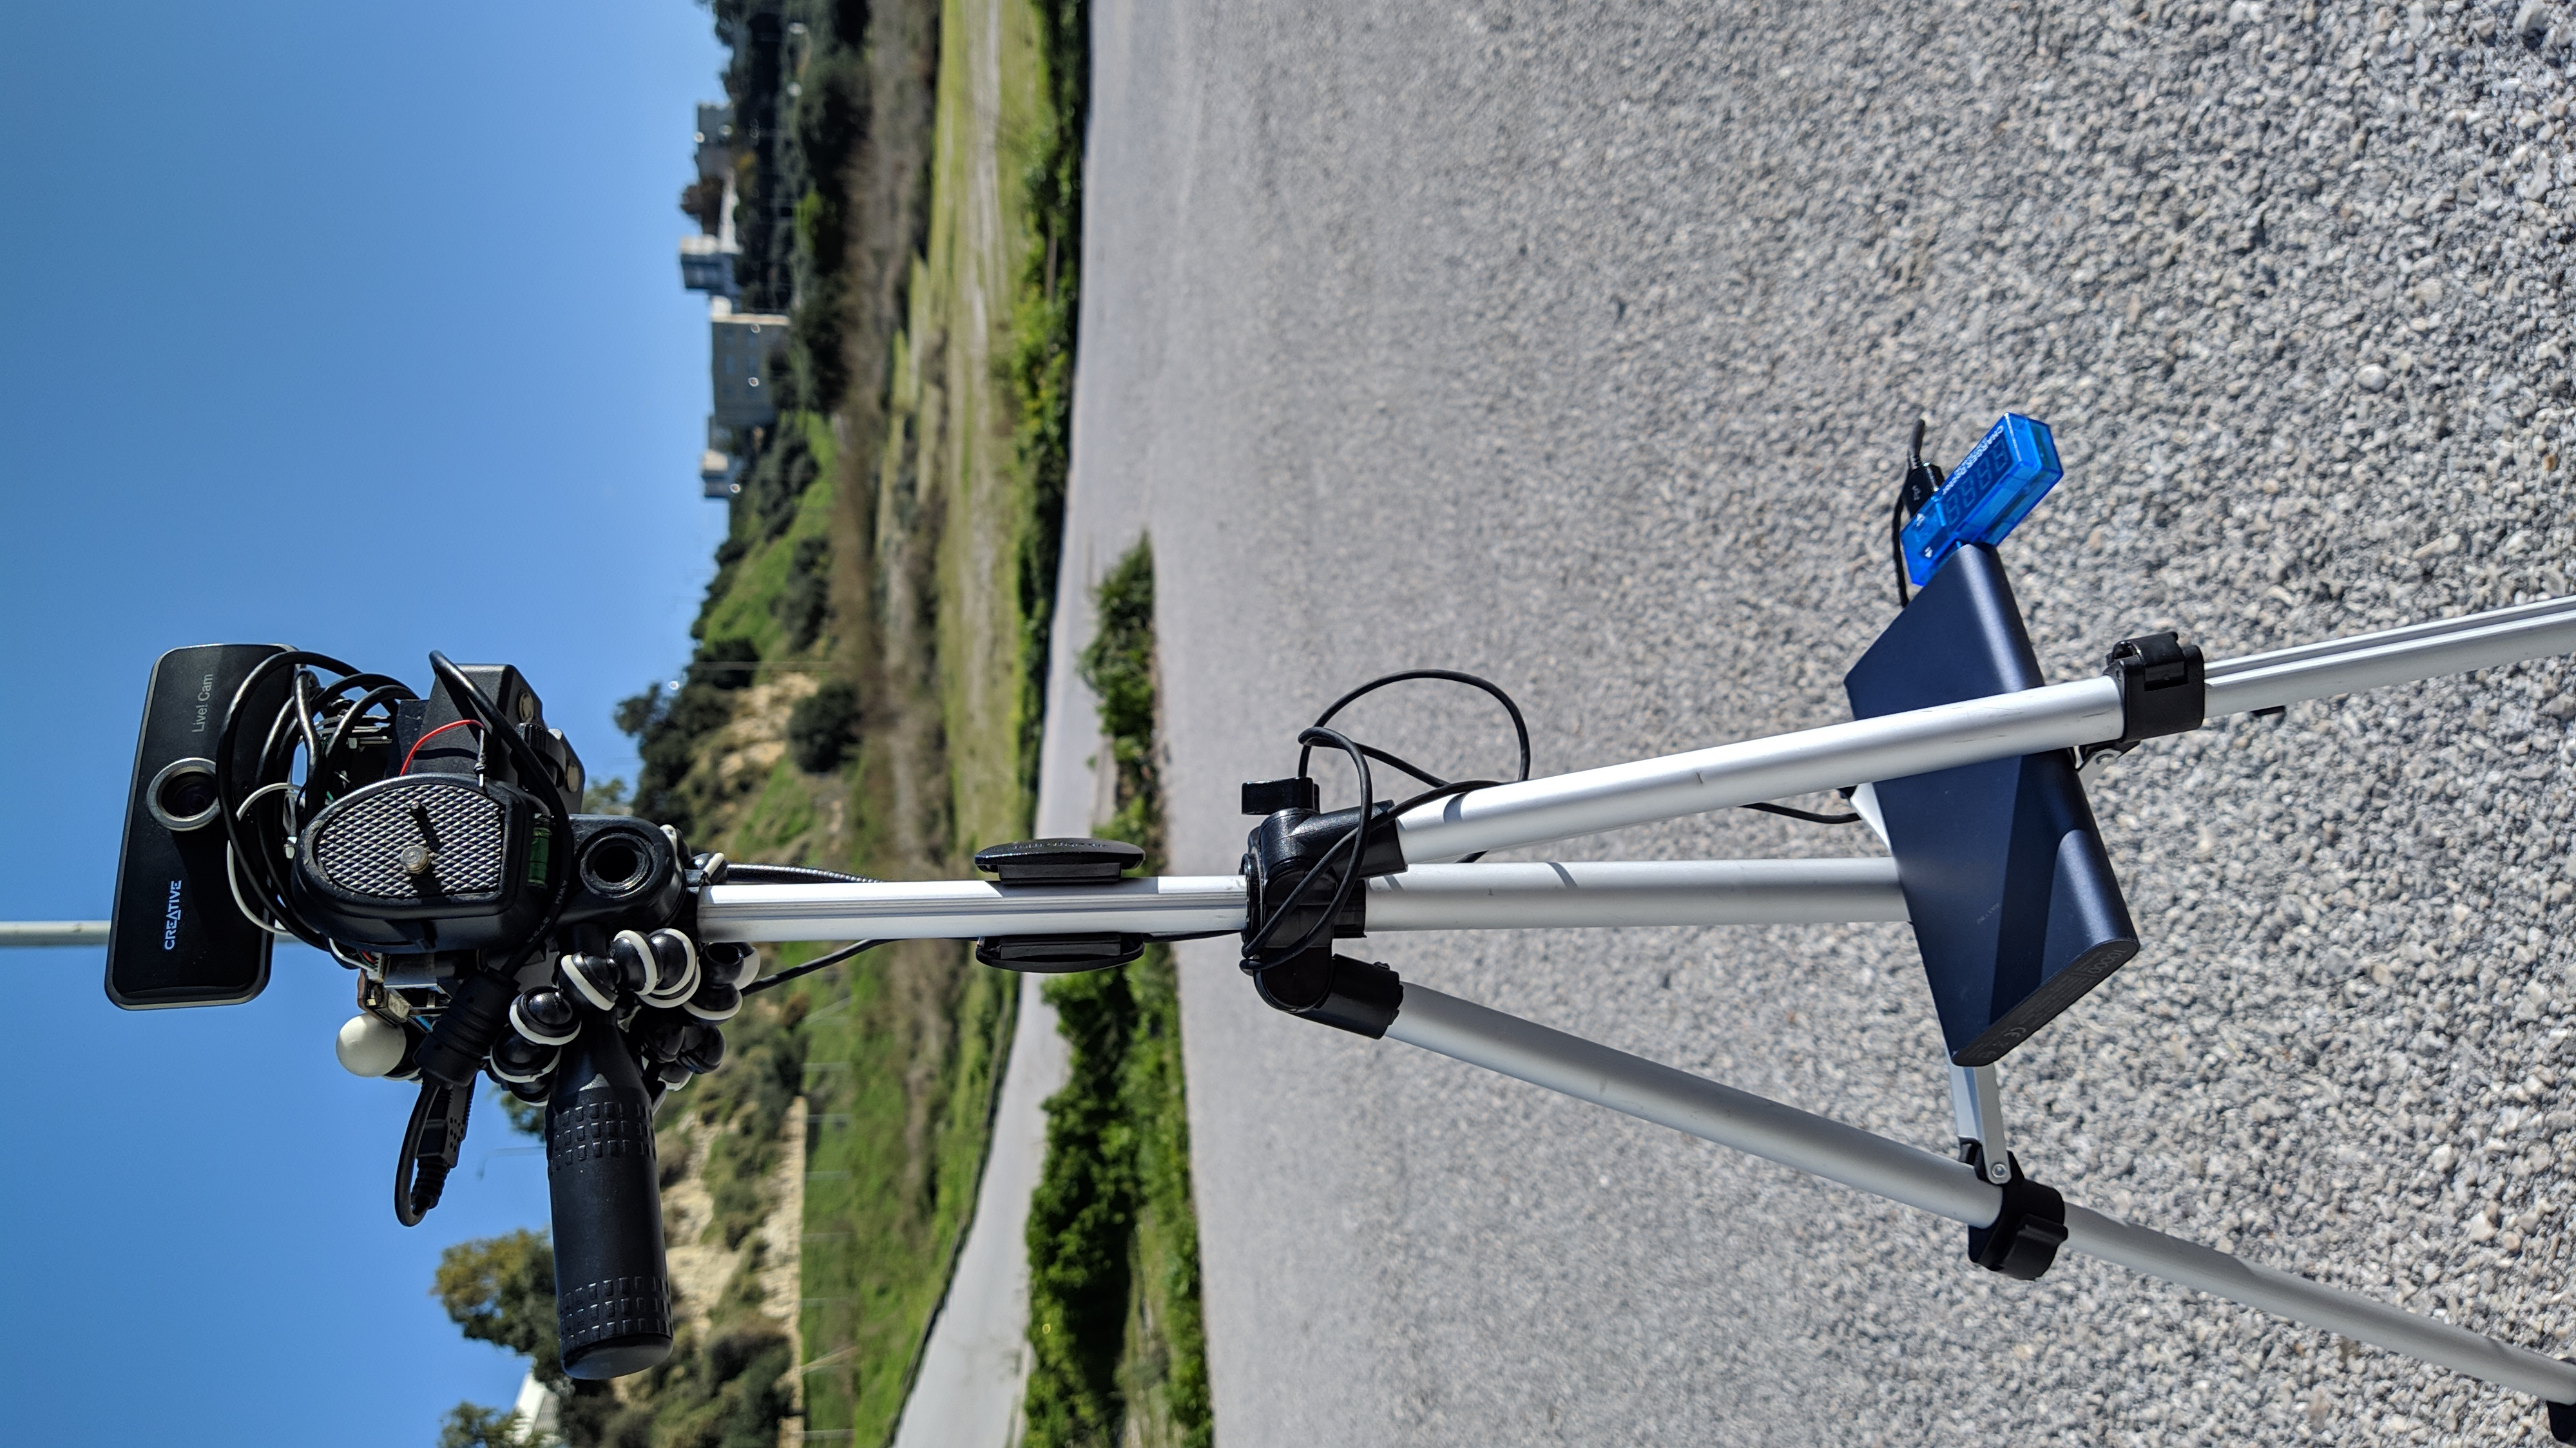
\includegraphics[width=\linewidth, angle =-90]{../Images/Experiments-Results/node.jpg} \\ \vspace{0.1cm}
      {(a) Υπό έλεγχο σύστημα (Node) το οποίο τροφοδοτείται από powerbank κατά την διάρκεια πειραμάτων}
    \end{minipage}%
    % -----------------
    \begin{minipage}{.5\textwidth}
      \centering
      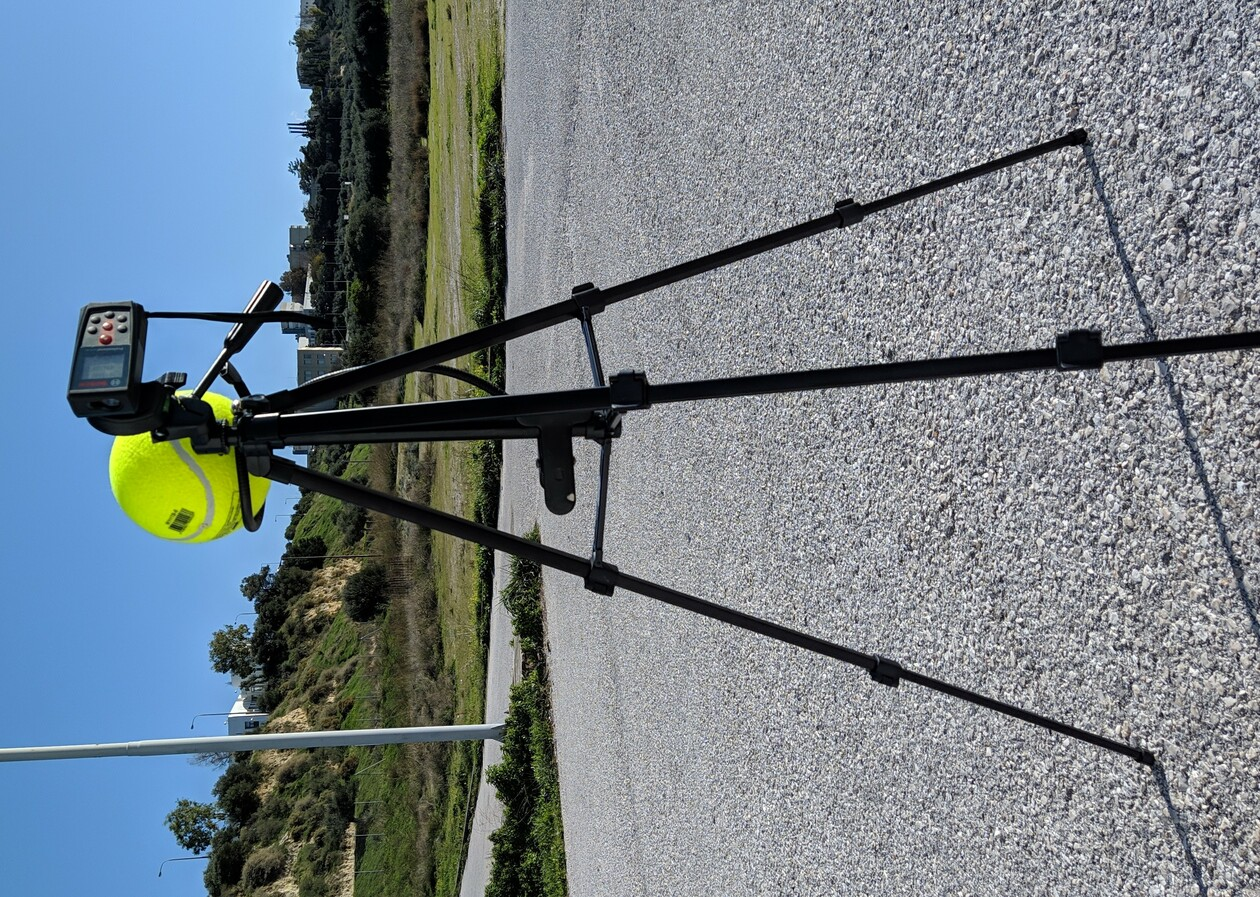
\includegraphics[width=\linewidth, angle =-90]{../Images/Experiments-Results/testing.jpg}\\ \vspace{0.1cm}
      {(b) Κινούμενο αντικείμενο εκτίμησης θέσης μαζί με το όργανο μέτρησης απόστασης }
	\end{minipage}
	% -----------------
    \hfill \break
    \decoRule
    \CaptionBasedwithURL{Εξοπλισμός που χρησιμοποιήθηκε στην πρώτη εξωτερική πειραματική φάση} 
    \label{fig:node-testing-env}
\end{figure}

Τα δύο αυτά αντικείμενα τοποθετήθηκαν το ένα απέναντι από το άλλο όπως φαίνεται στην \Fig{single-test-bench-side-view}, και πάρθηκαν μετρήσεις απόστασης για διαφορετικές γωνίες όπως φαίνεται στην 
\Fig{single-test-bench-angles}. Ταυτόχρονα, το σύστημα κατά την διάρκεια της διαδικασίας, ήταν σε πλήρη λειτουργία, και πραγματοποιούσε ανίχνευση και εκτίμηση της απόστασης του αντικειμένου από την κάμερα. Στη
\Sect{expe-single-3d} παρουσιάζονται τα πειραματικά αποτελέσματα των μετρήσεων αυτής της διαδικασία, ενώ στη 
\Sect{single-expe-system} παρουσιάζονται οι ανάγκες λειτουργίας από την σκοπιά του ε\-νσω\-μα\-τω\-μέ\-νου συστήματος.

\FigCaptLabelBasedURL{../Images/Experiments-Results/side.jpg}
{Χωρική τοποθέτηση του υπό ελέγχου συστήματος και αντικειμένου εκτίμησης θέσης}%
{single-test-bench-side-view}%
<0.8>

\FigCaptLabelBasedURL{../Images/Experiments-Results/testbench.png}
{Αναπαράσταση των θέσεων στις οποίες έγιναν οι μετρήσεις του πειράματος}%
{single-test-bench-angles}%
<0.6>

Όπως φαίνεται στην \Fig{node-testing-env} (b), το object το οποίο πρόκειται να εντοπίσουμε βρίσκεται σε τρίποδο, για μεγαλύτερη ευκολία των μετρήσεων, ενώ στο πλάγιο μέρος γίνεται διακριτό το όργανο που χρησιμοποιήθηκε για τον υπολογισμό της απόστασης μεταξύ των δύο αντικειμένων. Το όργανο αυτό είναι το laser range finder της Bosch GLM 40 - \Fig{bosch-range-estimator} - με δυνατότητες μέτρησης $0.15-40.00 m$ και απόκλιση μετρήσεων $\pm1.5mm$

Για τον υπολογισμό των διάφορων γωνιών από τις οποίες θα γινόντουσαν μετρήσεις, χρησιμοποιήθηκε το όργανο μέτρησης γωνιών όπως φαίνεται στην \Fig{single-test-bench-top-view}. Ενώ οι μετρήσεις που στην συνέχεια θα αναγερθούν αφορούν δεδομένα από γωνίες [$-20\si{\degree},-10\si{\degree},~0\si{\degree},~10\si{\degree},~20\si{\degree}$]\footnote{Λόγω του διαφορετικού ύψους μεταξύ της θέσης που μετρήθηκαν οι γωνίες και της κάμερας, δεν είναι οι ίδιες με αυτές που ανιχνεύονται στο x άξονα της εικόνας} και αποστάσεις μέτρησης ανά 50cm μέχρι τα 5m (εκτός από την κεντρική ευθεία στην οποία έγιναν μετρήσεις μέχρι περίπου τα 8m).

\FigCaptLabelBasedURL{../Images/Experiments-Results/glm40.jpg}
{Το ψηφιακό λέιζερ μέτρησης απόστασης που χρησιμοποιήθε (Bosch GLM 40)}%
{bosch-range-estimator}%
<0.4>%
(https://www.howetools.co.uk/bosch-glm-40-aaa-batteries-laser-range-finder)

\FigCaptLabelBasedURL{../Images/Experiments-Results/node-top-view.jpg}
{Υπολογισμός των γωνιών με χρήση εργαλείου μέτρησης γωνίας}%
{single-test-bench-top-view}%
<0.9>

% -------------------------------------------------------------
\subsection{Απόδοση του συστήματος} \label{sec:single-expe-system}

Πριν αναφερθούν τα δεδομένα που συλλέχθηκαν ως προς την απόδοση του συστήματος, θα αναφερθούν κάποια από τα 
χαρακτηριστικά λειτουργίας του. Η υλοποίηση του συστήματος έγινε σε C++. Δημιουργήθηκαν συνεπώς Function-like macros για εξαγωγή και αποθήκευση χρήσιμων πληροφοριών του συστήματος. Οι πληροφορίες που συλλέχθηκαν, αναφέρονται σε αυτήν την ενότητα, και σχετίζονται με τις επεξεργαστικές και ενεργειακές ανάγκες του συστήματος, η μνήμη μου χρειάζεται για να λειτουργήσει, και άλλες σημαντικές πληροφορίες.

Πρώτη από αυτές τις πληροφορίες είναι οι επεξεργαστικές ανάγκης του, όπου στην \Fig{cpu-usage-experiment-example}
φαίνονται τα δεδομένα που συλλέχθηκαν κατά την διάρκεια ενός από τα πειράματα. 

\FigCaptLabelBasedURL{../Images/Experiments-Results/raspberry-exp-cpu.png}
{Επεξεργαστική ισχύς του συστήματος}%
{cpu-usage-experiment-example}%
<1>

Μία ακόμα χρήσιμη μετρική είναι αυτή της μνήμης που χρησιμοποιεί το σύστημα, στην \Fig{ram-usage-experiment-example}
παρουσιάζεται η συγκεκριμένη πληροφορία. Από αυτό το διάγραμμα μπορούμε να παρατηρήσουμε ότι για την συγκεκριμένη υλοποίηση το σύστημα δεν έχει μεγάλες ανάγκες μνήμης\footnote{Έχοντας αυτήν την πληροφορία, μπορούμε να μεταβούμε σε επιλογή Embedded Linux System με μικρότερη μνήμη, που σημαίνει μικρότερο κόστος ανά node συστήματος}.
\FigCaptLabelBasedURL{../Images/Experiments-Results/raspberry-exp-ram.png}
{Ανάγκες μνήμης του συστήματος}%
{ram-usage-experiment-example}%
<1>

Το σύστημα αυτό σχεδιάζεται, με γνώμονα μελλοντικά να χρησιμοποιηθεί σε drones, συνεπώς οι ενεργειακές απαιτήσεις του είναι σημαντικές. Για αυτό τον λόγο ε\-ξά\-χθη\-καν και δεδομένα σχετικά με την κατανάλωση του συστήματος\footnote{Στις συγκεκριμένες γραφικές, μέχρι το 80s το σύστημα είναι σε idle mode, ενώ από εκεί και έπειτα είναι σε πλήρη λειτουργία} - \Fig{power-usage-experiment-example}. Με την μέγιστη κατανάλωση που παρατηρήθηκε από τροφοδοσία μέσω power bank κατά την διάρκεια δοκιμών είναι τα 10Watt, ενώ τάση τροφοδοσίας είναι τα 5Volt.
\FigCaptLabelBasedURL{../Images/Experiments-Results/raspberry-exp-power.png}
{Ενεργιακές απαιτήσεις συστήματος}%
{power-usage-experiment-example}%
<1>

Σημαντικός παράγοντας της απόδοσης ενός επεξεργαστή, είναι η θερμοκρασία του, καθώς αν είναι αυξημένη μπορεί η απόδοση να μειωθεί λόγω thermal throttling. Για αυτό συλλέχθηκε επίσης πληροφορία για την θερμοκρασία του επεξεργαστή - \Fig{temp-usage-experiment-example}. 
\FigCaptLabelBasedURL{../Images/Experiments-Results/raspberry-exp-temp.png}
{Θερμοκρασίες συστήματος έχοντας σε χρήση το fan του breakout board}%
{temp-usage-experiment-example}%
<1>

Ενώ τελευταία, αλλά εξίσου σημαντική μετρική, είναι ο υπολογισμός του χρόνου που χρειάζεται το σύστημα ανίχνευσης του αντικειμένου, για κάθε δευτερόλεπτο χρήσης του συστήματος, και παρουσιάζεται στην \Fig{hsv-calc-dur-experiment-example}.
\FigCaptLabelBasedURL{../Images/Experiments-Results/raspberry-exp-hsv-dur.png}
{Χρόνος του object detection μέσα σε κάθε δευτερόλεπτο χρήσης του συστήματος}%
{hsv-calc-dur-experiment-example}%
<1>

%----------------------------------------------------------------------

\subsection{Λαμβανόμενα δεδομένα και απεικόνιση} \label{sec:expe-single-3d}

Πριν αναφερθούν τα δεδομένα που λήφθηκαν κατά το πείραμα, είναι σημαντικό να γίνει κατανοητή η εξάρτηση pixel-απόστασης της σχέσης \EqNum{distance-from-object-pixels} που αναλύθηκε στο προηγούμενο κεφάλαιο και χρησιμοποιείται για το range estimation του αντικειμένου.

Η \Fig{pixel-dist-rel} παρουσιάζει την παραπάνω αναλογία, για τις παραμέτρους της κάμερας που χρησιμοποιήθηκε, σε αναλύσεις 1280x720 pixels.

\FigCaptLabelBasedURL{../Images/Experiments-Results/pixels-dist-rel.png}
{Εξάρτηση του μεγέθους του αντικειμένου σε pixel με απόσταση αντικειμένου από την κάμερα}%
{pixel-dist-rel}%
<1>

Αυτό που μπορούμε να παρατηρήσουμε είναι, ότι δεν είναι γραμμική. Όμως, μπορεί να προσεγγιστεί σε ένα υποσύνολο του πεδίο ορισμού της, με γραμμικό τρόπο. Αυτό σημαίνει ότι για σχετικά μεγάλες ακτίνες η μεταβολή σε pixel επιφέρει μικρές με\-τα\-βο\-λές στην απόσταση, ενώ για μικρές ακτίνες επιφέρει μεγάλες μεταβολές της απόστασης. 

Για λόγους πληρότητας θα δοθούν τρία παραδείγματα. Σε πολύ μικρές ακτίνες - λόγου χάρη για αντικείμενο ακτίνας 10 pixel - η εκτιμώμενη απόσταση είναι 12.4m, ενώ, αν το αντικείμενο εκτιμούσαμε ότι είχε ακτίνα 11 pixel, τότε η απόσταση θα ήταν 11.27m. Ως αποτέλεσμα, σε αυτήν την περίπτωση το 1 pixel σφάλματος του αντικειμένου στο image plane να καταλήγει σε 1.13m σφάλματος της εκτιμώμενης απόστασης στον φυσικό κόσμο. Για λίγο μεγαλύτερες ακτίνες, όπως για 50 pixel, η εκτιμώμενη απόσταση είναι 2.48m. Αν όμως για αυτή την ακτίνα του αντικείμενου είχαμε σφάλμα 1 pixel - δηλαδή μέτρηση 51 pixel - τότε η εκτιμώμενη απόσταση θα ήταν τα 2.43m, με τελικό σφάλμα τα 5cm σε αυτήν την περίπτωση. Τέλος, σε αρκετά μεγαλύτερες ακτίνες, με τα 100 pixel ως αναφορά, έχουμε εκτιμώμενη α\-πό\-στα\-ση τα 1.24m, ενώ, σε περίπτωση που η ακτίνα μας έχει 1 pixel διαφορά από την πραγματικότητα - δηλαδή έστω 101 pixels - και τα 1.22m εκτιμώμενη απόσταση, καταλήγουμε σε 2cm σφάλμα. Αυτό που βγαίνει ως συμπέρασμα από αυτήν την σχέση είναι ότι το τελικό σφάλμα εκτίμησης είναι σε άμεση εξάρτηση με το ποσοστό του image plane που καταλαμβάνει το αντικείμενο σε αυτό. 

Αφού έχει γίνει ξεκάθαρος αυτός ο περιορισμός, θα αναφερθούν τα δεδομένα που λήφθηκαν κατά την διάρκεια του πειράματος, από το node.
Αρχικά, στην \Fig{raspberry-exp-node-view} παρουσιάζεται στιγμιότυπο της αντιληπτικής ικανότητας - μεμονωμένης χρονικής στιγμής - του node, μαζί με τα διάφορα στάδια ε\-πε\-ξε\-ργα\-σίας, σε συνδυασμό με post-processing τρισδιάστατη απεικόνιση της μπάλας σε σχέση με την κάμερα (κάτω δεξιά στην εικόνα).

\FigCaptLabelBasedURL{../Images/Experiments-Results/node-view.png}
{Αντιληπτική ικανότητα μεμονωμένου κόμβου κατά την διάρκεια των δοκιμών, σε συνδυασμό με τρισδιάστατη απεικόνιση της μπάλας}%
{raspberry-exp-node-view}%
<1>

Οι γραφικές - \Fig{dist-experiment-example} και \Fig{angles-usage-experiment-example} - παρουσιάζουν τα raw data για την α\-πό\-στα\-ση και γωνίες που συλλέχθηκαν κατά την διάρκεια του πειράματος. Με την βοήθεια αυτών, μπορεί ακόμα και να φανεί η διαδρομή που ακολουθήθηκε κατά την διάρκεια του πειράματος. Επίσης, παρατηρείται να είναι σε ένα αρκετά μεγάλο ποσοστό κοντά στην πραγματική διαδρομή, με πολύ καλή προ\-σέ\-γγι\-ση για τον ε\-ντο\-πι\-σμό του αντικειμένου (όπως θα φανεί στην συνέχεια). Για τις οποίες, είναι σημαντικό όμως να αναφερθεί ότι τα spikes αναπαριστούν σημεία όπου δεν είχε γίνει ακριβές detection του object.

\begin{figure}[H]
  \centering
  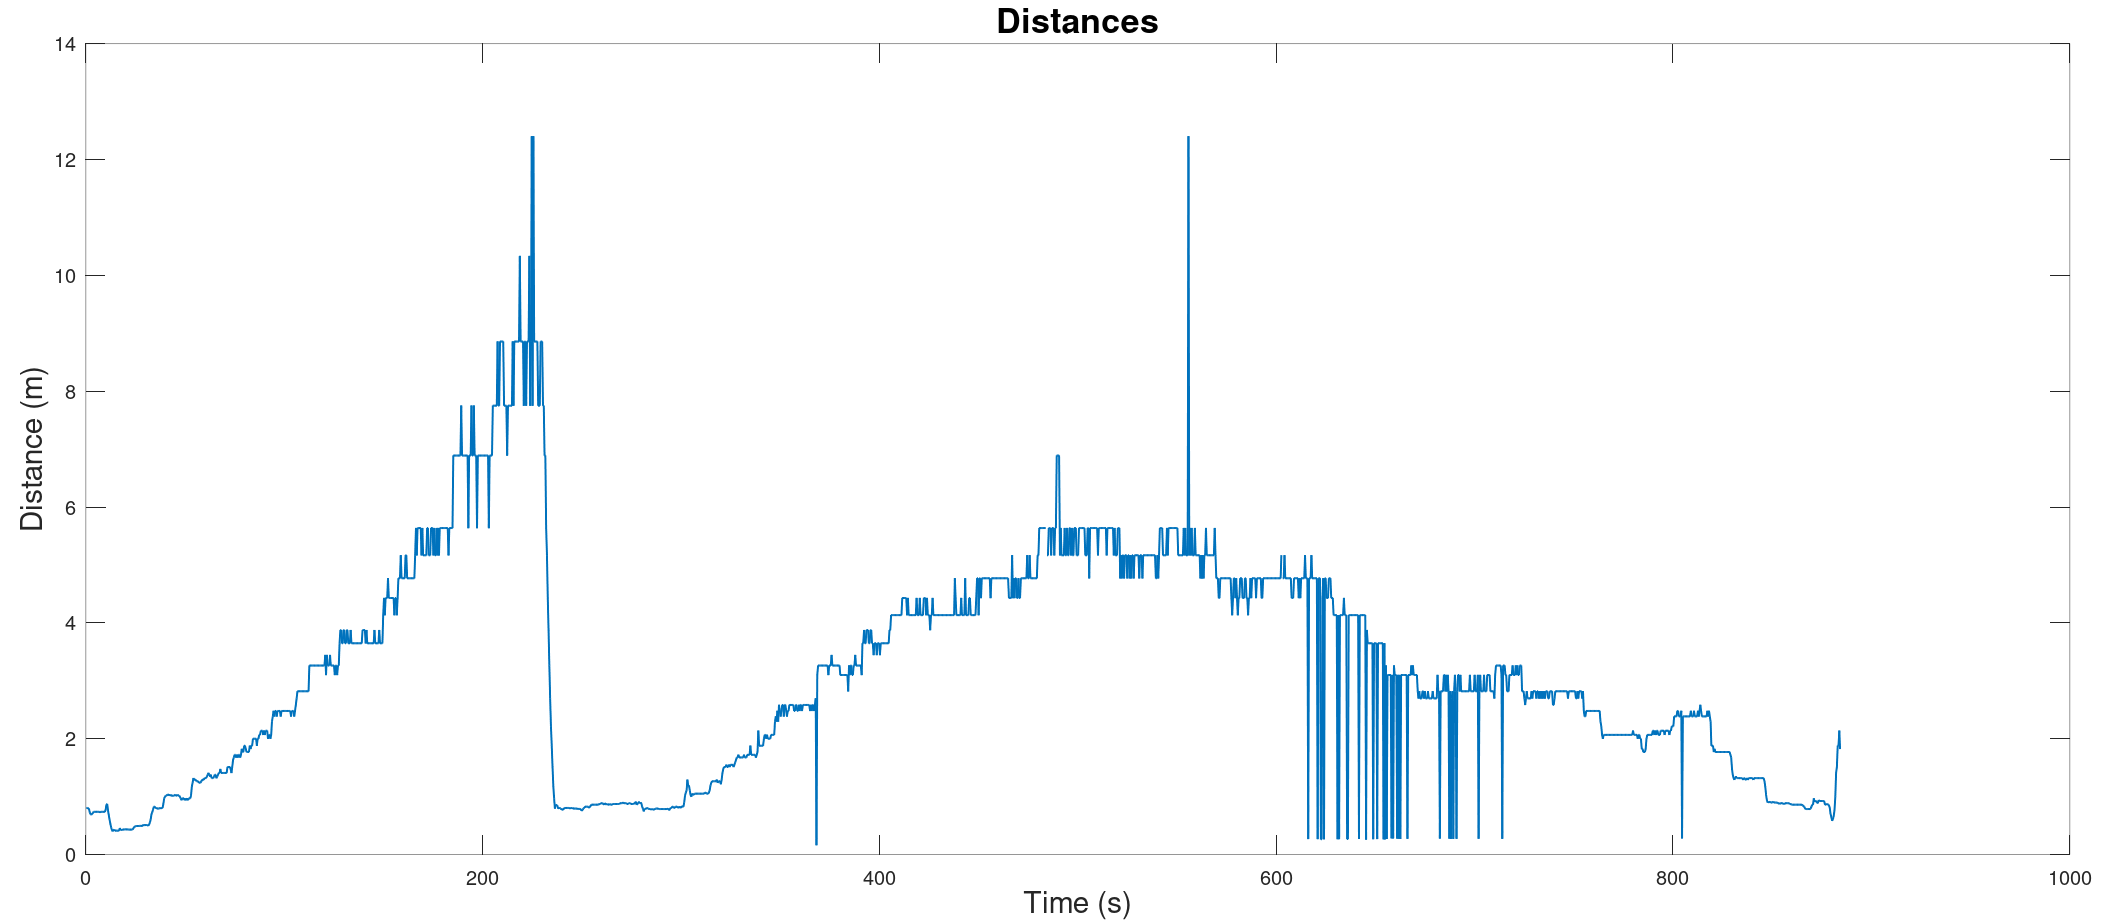
\includegraphics[width=\linewidth]{../Images/Experiments-Results/raspberry-exp-dist.png}
  \decoRule
  \caption[Εκτίμηση απόστασης για κάθε δευτερόλεπτο χρήσης του συστήματος]{Εκτίμηση απόστασης για κάθε δευτερόλεπτο χρήσης του συστήματος (για 3 από τις 5 ευθείες)}
  \label{fig:dist-experiment-example}
\end{figure}


\begin{figure}[H]
  \centering
  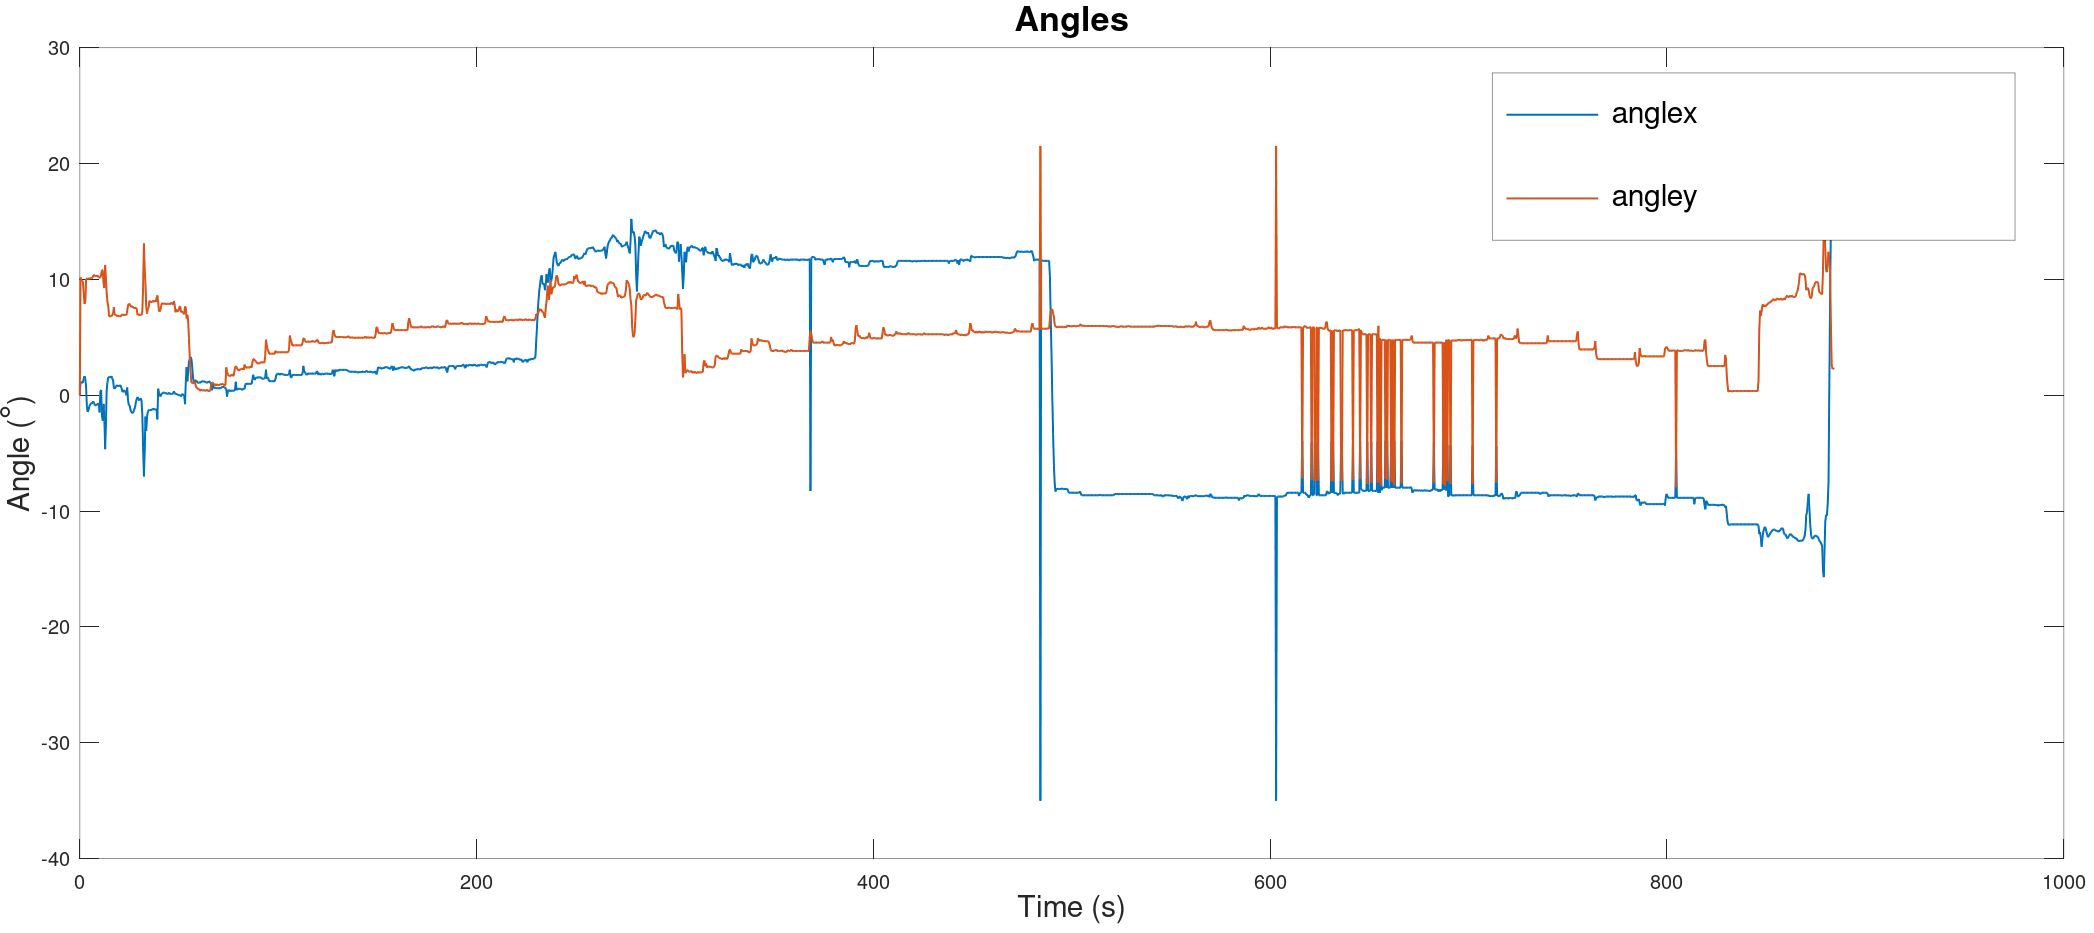
\includegraphics[width=\linewidth]{../Images/Experiments-Results/raspberry-exp-angles.png}
  \decoRule
  \caption[Εκτίμηση γωνιών στους άξονες x και y για κάθε δευτερόλεπτο χρήσης του συστήματος]{Εκτίμηση γωνιών στους άξονες x και y για κάθε δευτερόλεπτο χρήσης του συστήματος (για 3 από τις 5 ευθείες)}
  \label{fig:angles-usage-experiment-example}
\end{figure}

Με βάση τις δύο παραπάνω γραφικές, για την εκτίμηση απόστασης και γωνιών οι οποίες αποτελούν scalar τιμές, μπορούμε σε συνδυασμό - με απλή γεωμετρία - να αναπαραστήσουμε στο τρισδιάστατο χώρο όλες τις εκτιμήσεις για τις θέσης του αντικειμένου και να καταλήξουμε σε ένα vector θέσης ως προς την κάμερα. Αυτό γίνεται προσπάθεια να επιτευχθεί στην \Fig{obj-3d-repre}. Θεωρητικά θα μπορούσαμε μόνο με αυτόν τον τρόπο να εντοπίσουμε το αντικείμενο στον \Abbr{3D} χώρο, για λόγους α\-ξιο\-πι\-στίας όμως ωθούμαστε στον προσδιορισμό της θέσης από δεδομένα πολλαπλών κόμβων - από swarm - ώστε σε μία πιθανή αποστολή να μην έχουμε single point of failure. 

\FigCaptLabelBasedURL{../Images/Experiments-Results/raspberry-exp-obj-3d.png}
{Τρισδιάστατη απεικόνιση των μετρήσεων για 3 από τις 5 ευθείες}%
{obj-3d-repre}%
<1>

%----------------------------------------------------------------------

\section{Δεδομένα πολλαπλών κόμβων}
Όπως αναφέρθηκε και στη \Sect{GPS}, η λειτουργία του \Abbr{GPS} - τουλάχιστον σε αυτήν την φάση - ήταν για λόγους πληρότητας της υλοποίησης, ώστε να γίνει εύκολο το integration ενός \Abbr{GPS} με μικρότερο σφάλμα - όπως \Abbr{RTK} \Abbr{GPS} - σε μελλοντική υλοποίηση. Για αυτόν τον λόγο στην συνέχεια αναφερόμαστε σε καθορισμένων συντεταγμένων nodes.

%----------------------------------------------------------------------

\subsection{Διαδικασία λήψης δεδομένων} \label{sec:multiple-nodes-data-collection}
Στην συνέχεια πραγματοποιήθηκαν μετρήσεις από πολλαπλά σημεία (κόκκινα τε\-τρά\-γω\-να στο διάγραμμα) για το ίδιο αντικείμενο όπως παρουσιάζεται στην \Fig{multiple-nodes-positions}.
Με αυτόν τον τρόπο, για την ίδια θέση της μπάλας (με μαύρο χρώμα στο διάγραμμα) θα μπορούσε να προσομοιωθούν - σε ένα πρώιμο τουλάχιστον στάδιο - τα δεδομένα που δημιουργούνται από πολλαπλούς κόμβους σε ένα σμήνος από drone. 

\FigCaptLabelBasedURL{../Images/Experiments-Results/nodes-pos.png}
{Απεικόνιση των θέσεων από τις οποίες πραγματοποιήθηκαν λήψεις, καθώς και οι θέσεις του αντικειμένου}%
{multiple-nodes-positions}%
<.8>

Για κάθε μία από αυτές τις θέσεις πάρθηκαν μετρήσεις απόστασης μέσω που laser range finder που αναφέρθηκε παραπάνω (\Fig{bosch-range-estimator}) καθώς επίσης καταγράφηκαν και οι εκτιμήσεις αποστάσεις που πραγματοποιήθηκαν από το σύστημα. Στο \Tabl{multiple-nodes-est-act-dist} παρουσιάζονται αναλυτικά αυτές οι μετρήσεις, ενώ στην \Fig{est-act-dist-figure} γίνεται οπτικοποίηση τους.

Επίσης, στην \Fig{multiple-nodes-perception} δίνεται παράδειγμα της αντιληπτικής ικανότητας του κάθε κόμβου, όταν έχει τοποθετηθεί στην θέση 2 (βλ. \Fig{multiple-nodes-positions}) το αντικείμενο.

% TABLE
\begin{table}[H]
  \caption[Πραγματικές αποστάσεις και εκτιμήσεις για κάθε γωνία λήψης]{Πραγματικές αποστάσεις και εκτιμήσεις για κάθε γωνία λήψης} \label{tab:multiple-nodes-est-act-dist}
  \centering
  \resizebox{0.9\textwidth}{!}{
    \begin{tabular}{ccccccccc}
        \toprule
        & \multicolumn{2}{c}{Node 1} & \multicolumn{2}{c}{Node 2} & \multicolumn{2}{c}{Node 3} & \multicolumn{2}{c}{Node 4} \\
        \midrule
    pos & Estimation      & Real     & Estimation      & Real     & Estimation      & Real     & Estimation      & Real     \\
    \midrule
    1   & 1.886 & 1.820 & 1.927 & 1.847 & 1.809 & 1.765 & 1.886 & 1.839 \\
    2   & 1.248 & 1.539 & 1.343 & 1.560 & 2.333 & 2.475 & 2.273 & 2.510 \\
    3   & 2.273 & 2.488 & 1.198 & 1.507 & 1.231 & 1.514 & 2.396 & 2.499 \\
    4   & 2.333 & 2.471 & 2.333 & 2.519 & 1.182 & 1.469 & 1.323 & 1.515 \\
    5   & 1.248 & 1.510 & 2.396 & 2.522 & 2.162 & 2.396 & 1.182 & 1.532 \\
    6   & 1.641 & 1.593 & 2.162 & 2.146 & 2.014 & 2.040 & 1.555 & 1.617 \\
    7   & 1.502 & 1.473 & 1.970 & 1.927 & 2.162 & 2.157 & 1.773 & 1.870 \\
    8   & 1.611 & 1.627 & 1.672 & 1.643 & 2.110 & 2.071 & 2.061 & 2.139 \\
    9   & 1.847 & 1.914 & 1.528 & 1.478 & 1.809 & 1.831 & 2.110 & 2.223 \\
    10  & 2.061 & 2.129 & 1.611 & 1.610 & 1.583 & 1.568 & 2.110 & 2.155 \\
    11  & 2.162 & 2.209 & 1.886 & 1.919 & 1.453 & 1.427 & 1.886 & 1.877 \\
    12  & 2.162 & 2.138 & 2.110 & 2.168 & 1.528 & 1.547 & 1.611 & 1.591 \\
    13  & 1.847 & 1.837 & 2.273 & 2.225 & 1.773 & 1.836 & 1.528 & 1.488 \\
    \bottomrule
    \end{tabular}
}
\end{table}

\begin{figure}[H]
  \centering
  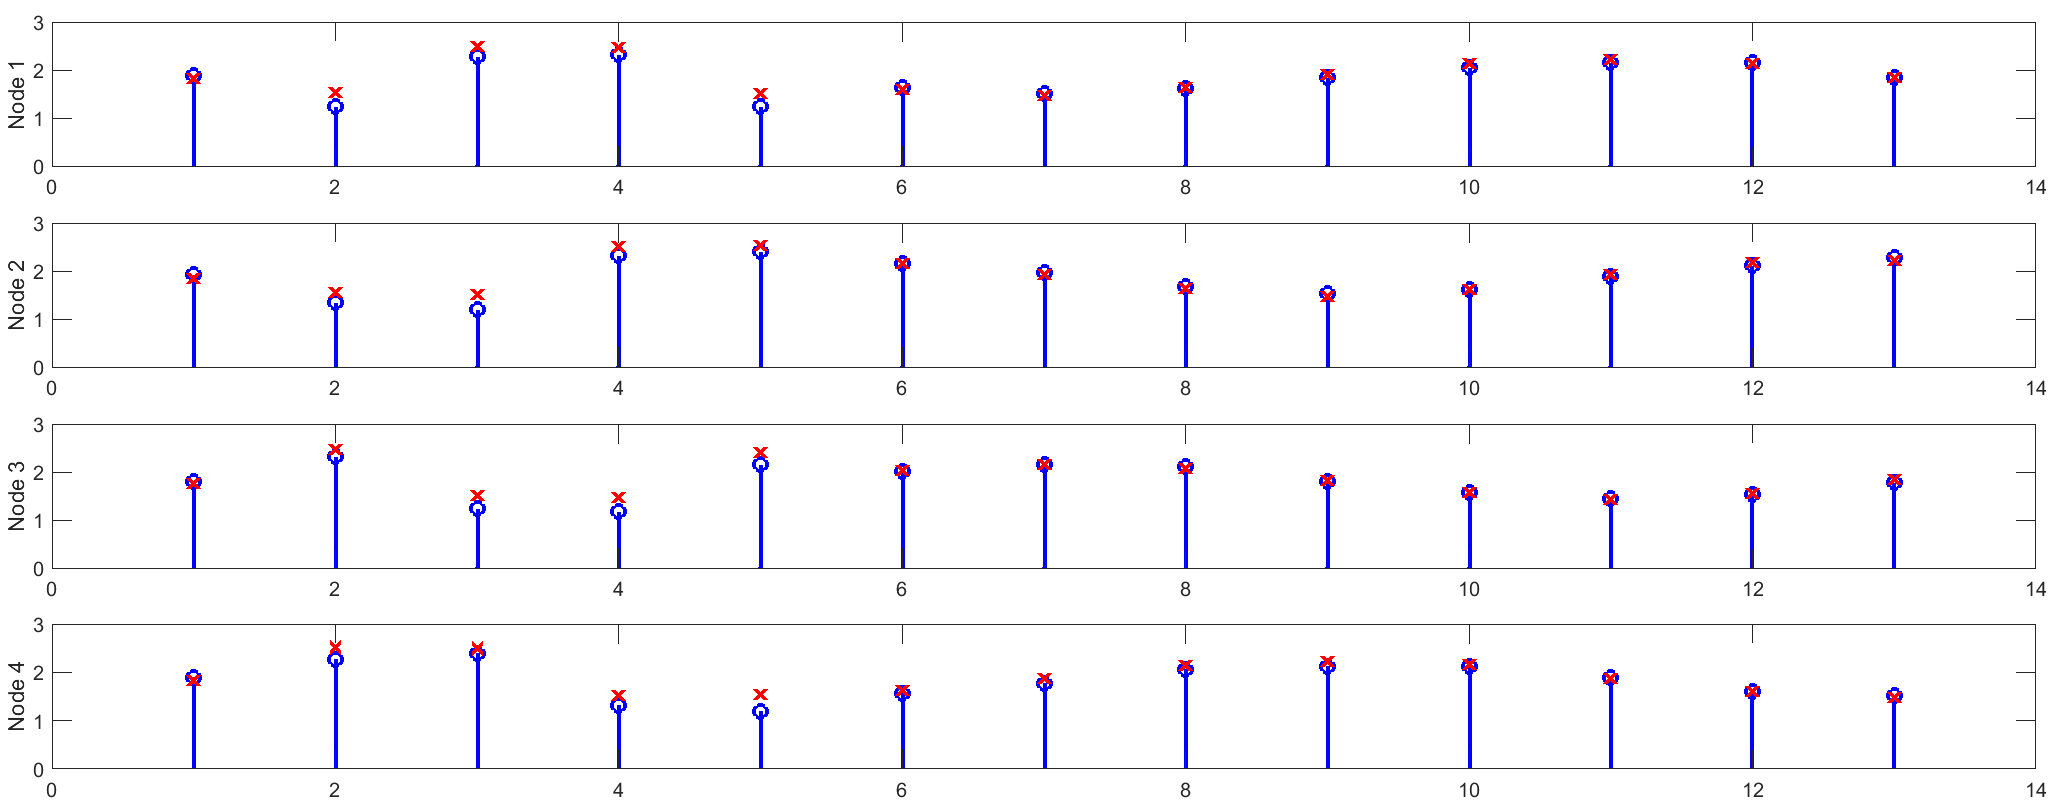
\includegraphics[width=0.9\linewidth]{../Images/Experiments-Results/nodes-estimations.png}
  \decoRule
  \caption[Γραφική αναπαράσταση της εκτίμησης θέσης - πραγματικής απόστασης]{Γραφική αναπαράσταση της εκτίμησης θέσης - πρα\-γμα\-τι\-κής απόστασης (Σύμφωνα με τα δεδομένα του \Tabl{multiple-nodes-est-act-dist}, όπου \textcolor{blue}{o} οι εκτιμήσεις και \textcolor{red}{x} οι πραγματικές αποστάσεις)}
  \label{fig:est-act-dist-figure}
\end{figure}

Από τις παραπάνω μετρήσεις καταλήγουμε σε συνολικό μέσο όρο σφάλματος τα 0.0974 m. Αν διαχωρίσουμε το σφάλμα, με βάση τις εξωτερικές (2-5) και εσωτερικές (1 και 6-13) θέσεις τότε μπορούμε να καταλήξουμε σε δύο επιπλέον σφάλματα. Για τις εξωτερικές ο μέσος όρος των σφαλμάτων είναι τα 0.2230m ενώ για τις εσωτερικές τα 0.0686m. Ο λόγος που συμβαίνει αυτό, σχετίζεται με την παραμόρφωση που προκαλεί ο φακός της κάμερας (με μεγαλύτερες επιδράσεις προς τα άκρα του image plane), και δεν έγινε εφικτό μέσω του calibration να διορθωθεί.

\FigCaptLabelBasedURL{../Images/Experiments-Results/multiple-nodes/combined/low-res/p2.png.low.png}
{Αντιληπτική ικανότητα από κάθε γωνία λήψης για την θέση 2}%
{multiple-nodes-perception}%
<1>

%----------------------------------------------------------------------

\subsection{Εκτίμηση θέσης και απεικόνιση}
Έχοντας συλλέξει τα δεδομένα που αναφέρθηκαν στη \Sect{multiple-nodes-data-collection}, μπορούσε να χρησιμοποιηθεί ο φορμαλισμός που περιγράφηκε στη \Sect{implementation-obj-mult} για την εκτίμηση της θέσης στον τρισδιάστατο χώρο. 

Χρησιμοποιήθηκαν 4 nodes - με ένα από αυτά να αποτελεί ταυτόχρονα χρέη master και worker node - όπου έστελναν στο σύστημα επαναλαμβανόμενα τα ranges και positions του κάθε node που αναφέρθηκαν παραπάνω, με τον τρόπο που περιγράφηκε στο προηγούμενο κεφάλαιο. Αφού το master λάβει τα πακέτα και πραγματοποιήσει την επεξεργασία, χρησιμοποιεί \textbf{geometry\_msgs/Pose} - αποτελεί ένα από τις βασικές μορφές μηνυμάτων για θέση του \Abbr{ROS} - για να γνωστοποιηθεί στο δίκτυο την εκτίμηση της θέση της μπάλας.

Σύμφωνα με τα παραπάνω, στην \Fig{exp-topics-nodes} φαίνονται τα περιεχόμενα των topic κατά την διαδικασία του πειράματος, ενώ στην \Fig{multi-exp-pos-estimations} μπορούμε να δούμε συνδυαστικά τις γραφικές, στις οποίες παρουσιάζονται οι θέσεις που βρισκόταν το αντικείμενο, καθώς και οι εκτιμήσεις της θέσης που τελικά προέκυψαν.

Από τις εκτιμήσεις και τις ακριβής θέσεις, μπορούμε τελικά να υπολογίσουμε το συνολικό σφάλμα του συστήματος. Για το οποίο καταλήγουμε, ότι το συνολικό σφάλμα εκτίμησης θέσης από το σμήνος να είναι τα 0,1159m.

\begin{figure} [H]
	\centering
	% -----------------
    \begin{minipage}{.5\textwidth}
      \centering
      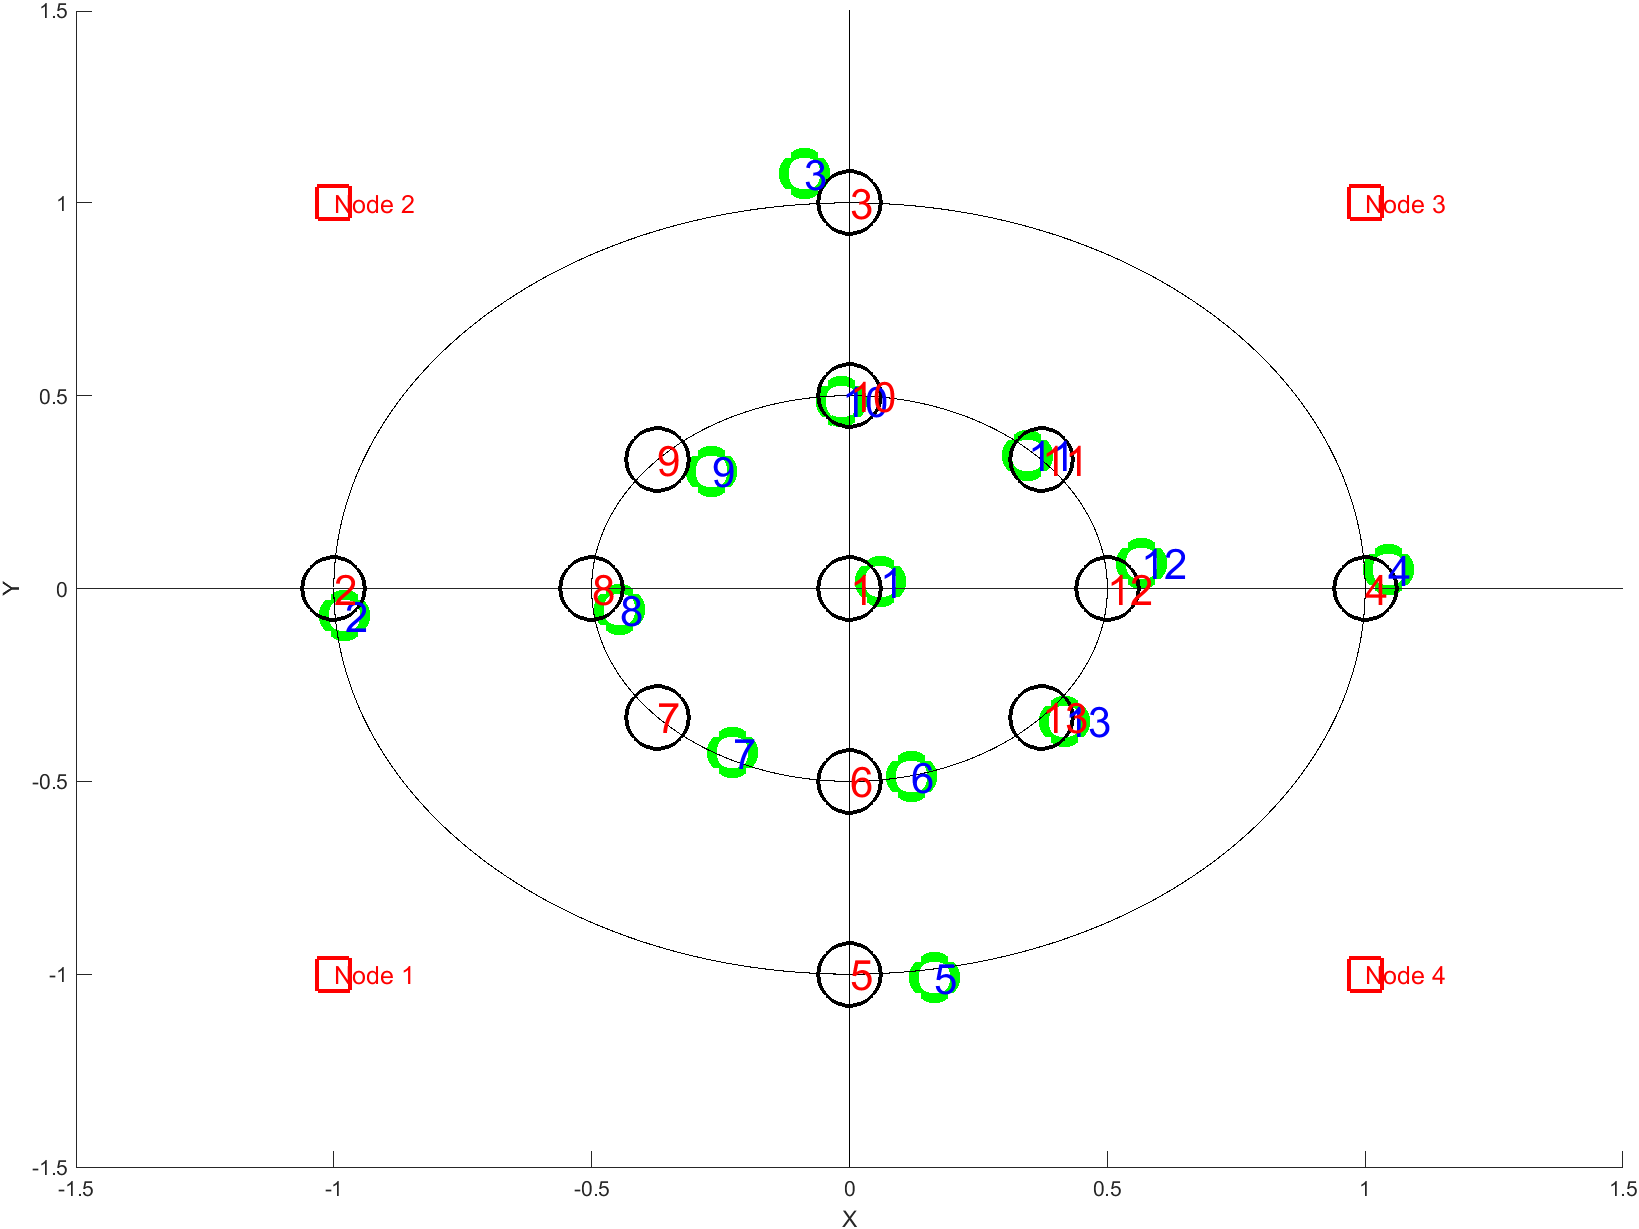
\includegraphics[width=0.9\linewidth]{../Images/Experiments-Results/nodes-pos-with-est-up.png}\\
      {(a) Top View}
    \end{minipage}%
    % -----------------
    \begin{minipage}{.5\textwidth}
      \centering
      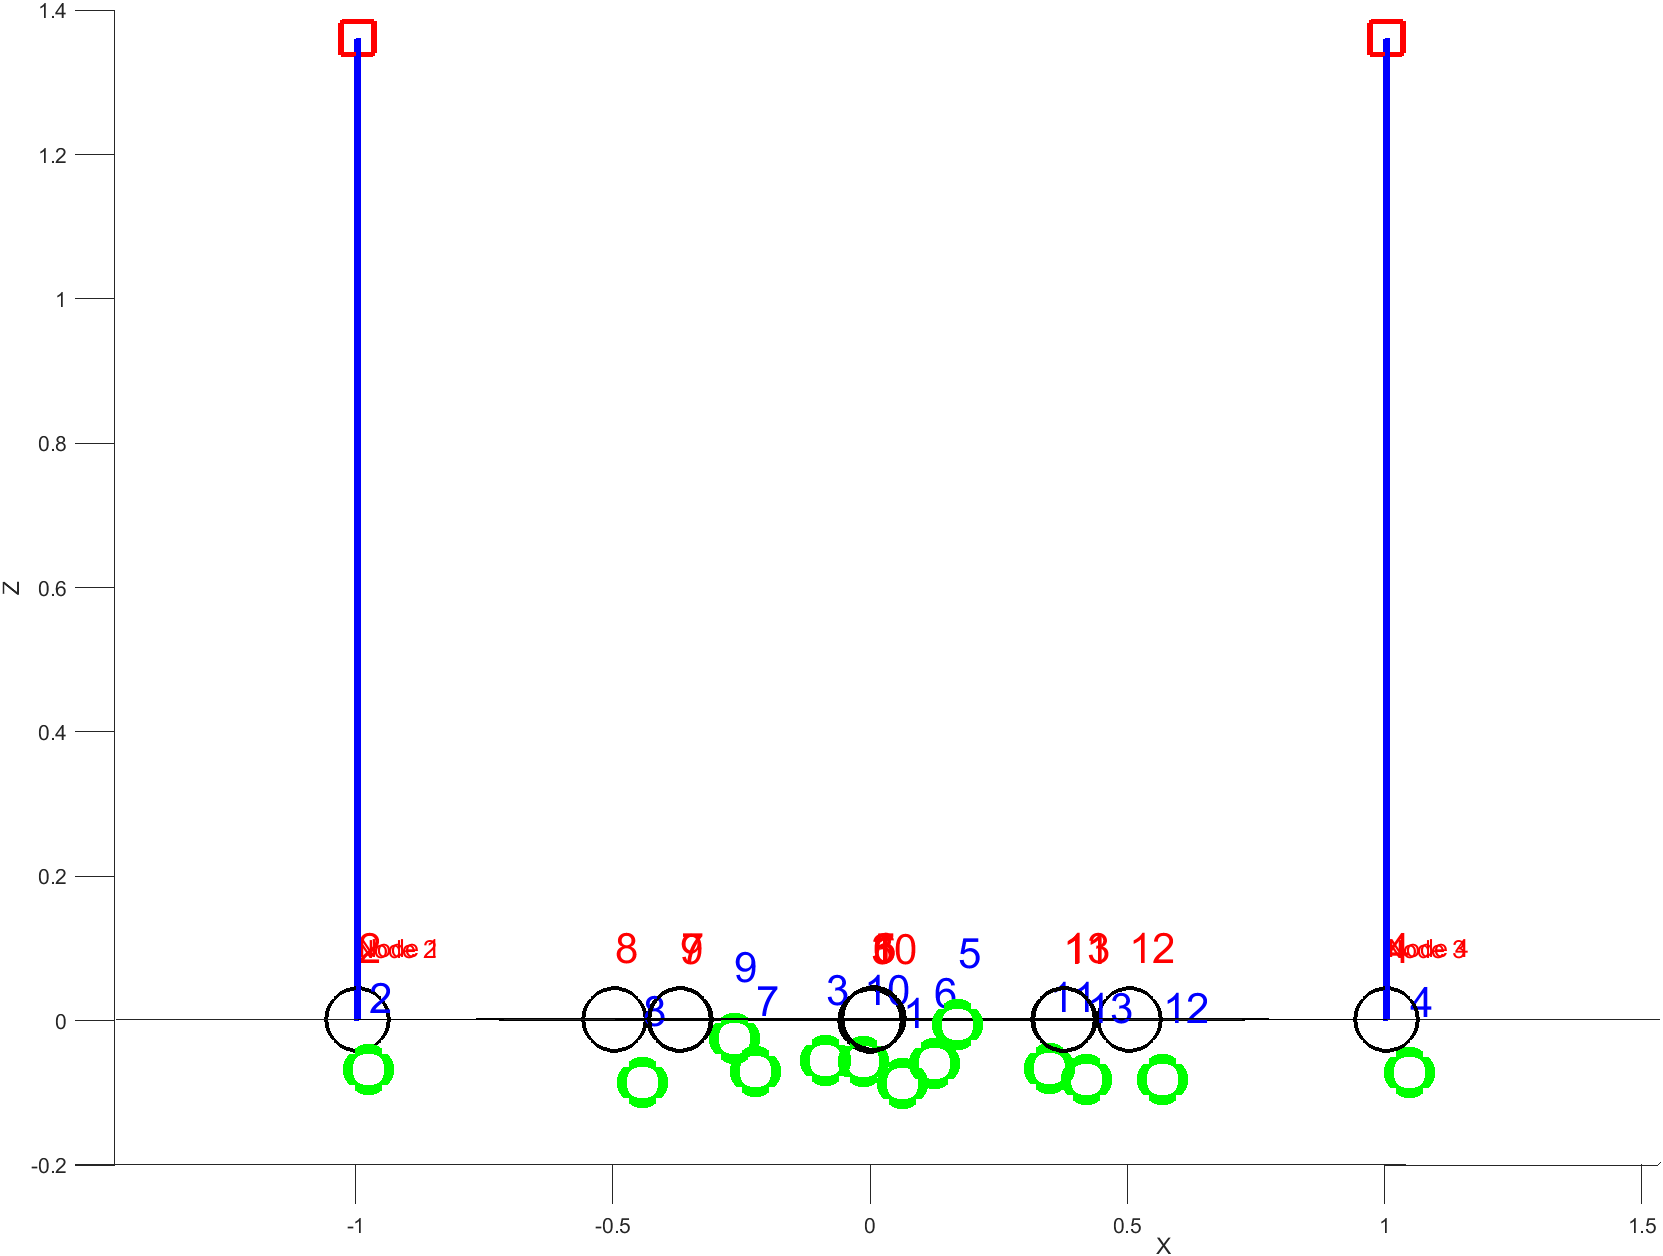
\includegraphics[width=.9\linewidth]{../Images/Experiments-Results/nodes-pos-with-est-side.png}\\
      {(b) Side View}
	  \end{minipage}
	% -----------------
  \begin{minipage}{\textwidth}
    \centering
    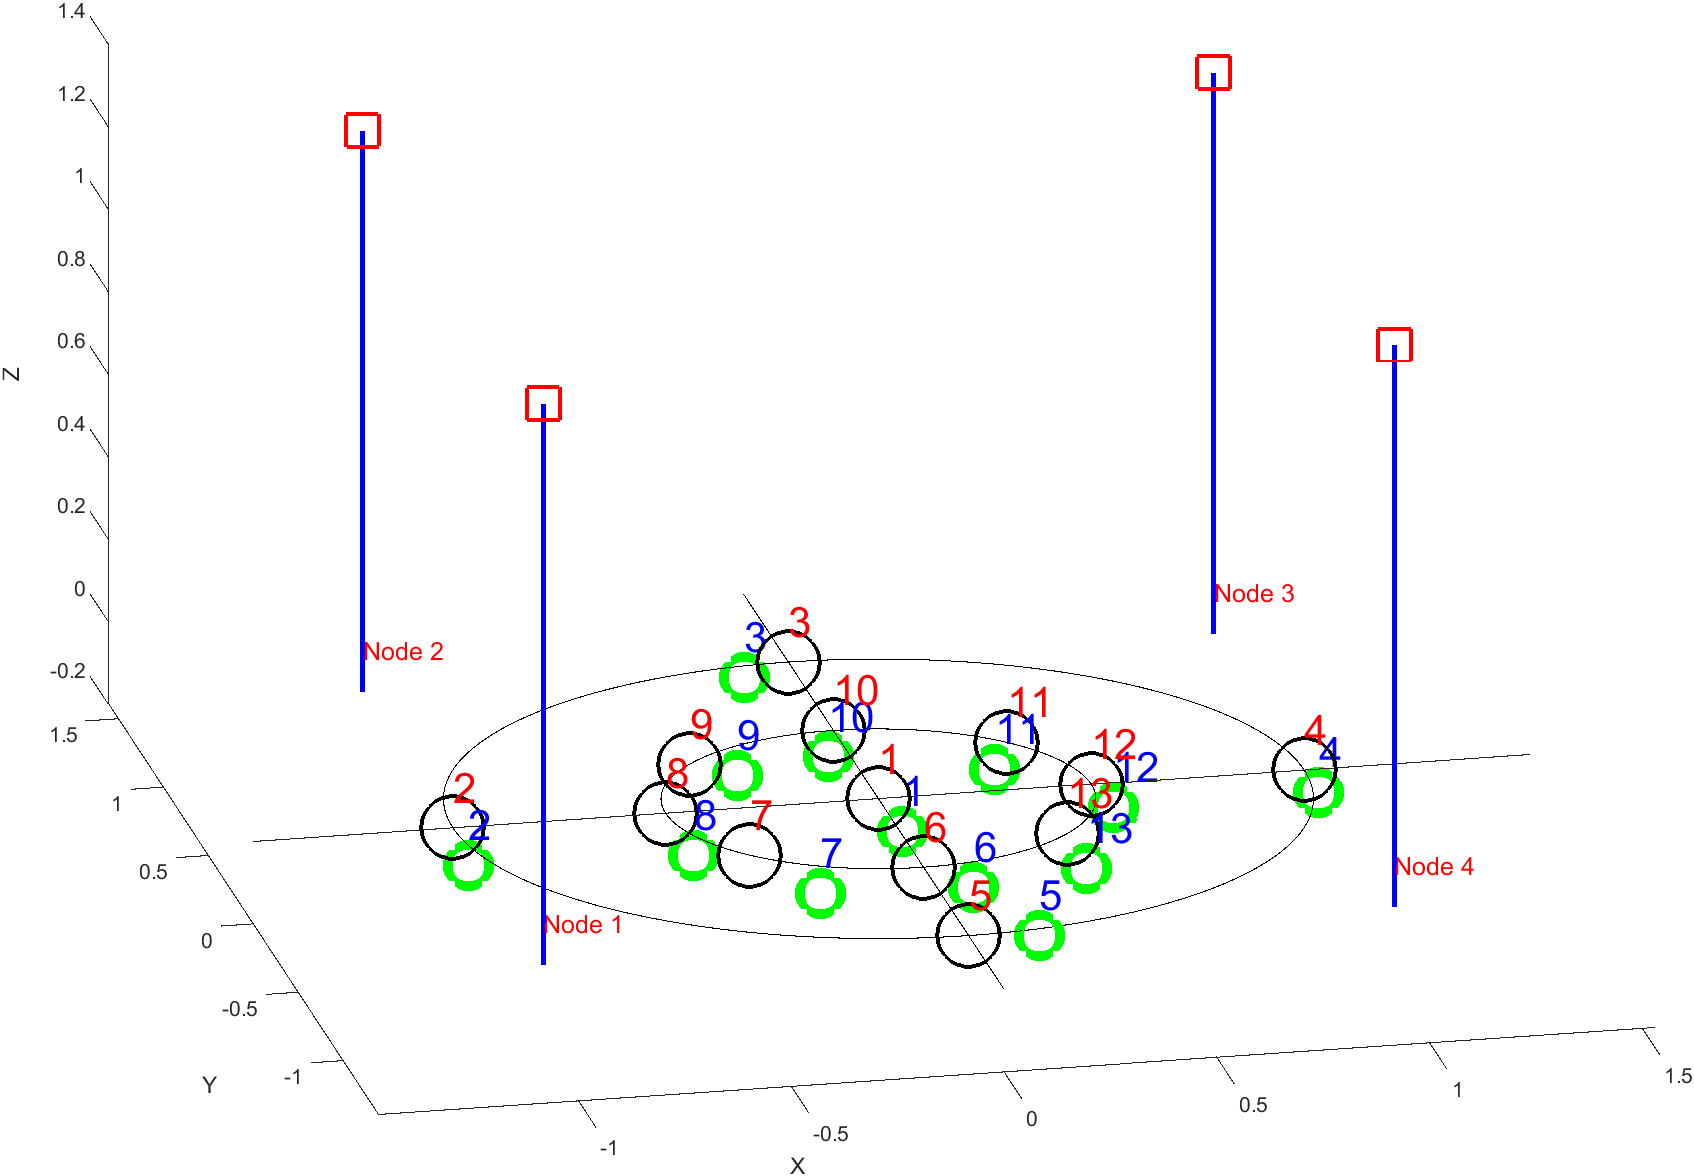
\includegraphics[width=.8\linewidth]{../Images/Experiments-Results/nodes-pos-with-est-angle.png}\\
    {(C) Angled View}
  \end{minipage}
% -----------------
    \hfill \break
    \decoRule
    \caption[Εκτίμηση θέσης του αντικειμένου.]{Εκτίμηση θέσης του αντικειμένου. Με \textcolor{black}{\LARGE$\circ$} είναι οι θέσεις στις οποίες τοποθετήθηκε το αντικείμενο ενώ με \textcolor{green}{\LARGE$\circ$} είναι οι θέσεις που έγινε εκτίμηση ότι βρίσκεται} %\CaptionBasedwithURL{Possible Embedded Linux Systems} 
    \label{fig:multi-exp-pos-estimations}
\end{figure}

\FigCaptLabelBasedURL{../Photos/topics.wr.png}
{Μέρος των εν λειτουργία nodes/topics, καθώς και απεικόνιση των πληροφοριών που αποστέλλουν στα topics τα 4 nodes, μαζί με την εκτίμηση της θέσης από τον master.}%
{exp-topics-nodes}%
<1>

%----------------------------------------------------------------------

\section{Επαλήθευση προσδιορισμού ID}
Όπως αναφέρθηκε στη \Sect{id-estimation} χρησιμοποιούμε την συχνότητα με την οποία αναβοσβήνει το led για τον καθορισμό του ID\footnote{Βίντεο από την διαδικασία του πειράματος μπορεί να βρεθεί στο \cite{experiment-blink-video}}. Σημαντικός παράγοντας για την επιλογή της συχνότητας είναι το frame-rate της κάμερας με την οποία δειγματοληπτούμε. 

Από το Nyquist–Shannon sampling theorem γνωρίζουμε ότι πρέπει να ισχύει $f_s > 2f_{max}$ μεταξύ της συχνότητας δειγματοληψίας και της μέγιστης συχνότητας σε ένα σήμα. Στην πράξη, είναι συχνό φαινόμενο να επιλέγουμε να διαφέρουν ακόμα και μία τάξη μεγέθους στην παραπάνω ανίσωση. Λόγω των 30fps της κάμερας καταλήγουμε να έχουμε ανά περίπου 33.33ms νέο καρέ, συνεπώς επιλέχθηκε ο χρόνος για τον οποίο θα είναι ενεργοποιημένο το led να είναι τα 70ms ώστε να καταγράφεται από τουλάχιστον 2 καρέ η ενεργοποίηση του. 

Για τις περιόδους ανάλογα με το ID επιλέχθηκαν οι χρόνοι 500ms για ID = 1, 1500ms για ID = 2, 2500ms για ID = 3, κλπ., ώστε να υπάρχει ένα περιθώριο 1000ms για πιθανά σφάλματα μεταξύ των μετρήσεων. 

Η \Fig{id-osci-samples} παρουσιάζει τους παλμούς στους οποίους ενεργοποιείται το led, και κρατάμε αποδεκτό το ID = 1 για durations μεταξύ των παλμών durations <= 1000ms, όμοια για ID = 2 έχουμε 1000ms < duration <= 2000ms, κλπ.

\begin{figure} [H]
	\centering
	% -----------------
    \begin{minipage}{.5\textwidth}
      \centering
      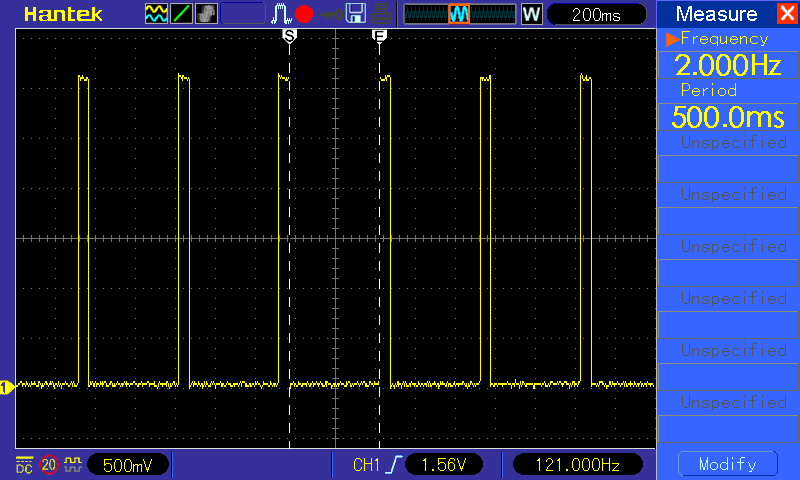
\includegraphics[width=0.9\linewidth]{../Images/Experiments-Results/node-pulses-0_5sec.png}\\
      {(a) Συχνότητα του led για ID = 1}
    \end{minipage}%
    % -----------------
    \begin{minipage}{.5\textwidth}
      \centering
      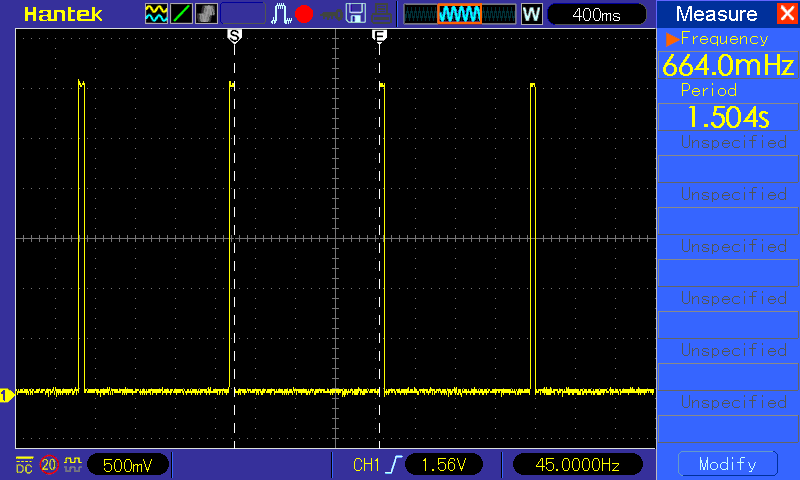
\includegraphics[width=.9\linewidth]{../Images/Experiments-Results/node_pulses_1_5sec.png}\\
      {(b) Συχνότητα του led για ID = 2}
	  \end{minipage}
% -----------------
    \hfill \break
    \decoRule
    \caption[Παράδειγμα δύο εκ των τεσσάρων συχνοτήτων για την λειτουργία του led που επιλέχθηκαν.]{Παράδειγμα δύο εκ των τεσσάρων συχνοτήτων για την λειτουργία του led που επιλέχθηκαν.}%\CaptionBasedwithURL{Possible Embedded Linux Systems} 
    \label{fig:id-osci-samples}
\end{figure}

Τέλος, η \Fig{exp-led-freq} παρουσιάζει στιγμιότυπο κατά την διαδικασία επαλήθευσης της λειτουργίας, στο οποίο παρουσιάζεται τόσο το ID που εκτιμήθηκε όσο και το duration μεταξύ την παλμών.

\FigCaptLabelBasedURL{../Images/Experiments-Results/frequency-analysis.png}
{Στιγμιότυπο της διαδικασίας πείραματος, κατά την διάρκεια καθορισμού του ID του αντικειμένου με βάση την συχνότητα που αναβοσβήνει το led}%
{exp-led-freq}%
<.8>

Από τα παραπάνω πειράματα, δείχνεται ότι είναι εφικτός ο προσδιορισμός της θέσης της μπάλας. Παρόλα αυτά, λόγω των περιορισμών που αναφέρθηκαν, σε αυτήν την μορφή που βρίσκεται ακόμα το σύστημα, συμπεραίνουμε ότι πρα\-γμα\-το\-ποι\-εί τις βέλτιστες προσεγγίσεις της θέσης, όταν το αντικείμενο ανιχνεύεται περίπου στο μέσω του image plane σε αποστάσεις κάτω των 5m.

Ακόμα, ενώ μπορεί να προσδιοριστεί μοναδικά το ID του αντικειμένου που εντοπίζεται, είναι φανερό ότι ο χρόνος που χρειάζεται ώστε αξιόπιστα να καθοριστεί αυτό\udot δεν είναι πεπερασμένος και μπορεί να χρειαστεί μερικά δευτερόλεπτα. Ο οποίος εξαρτάται από το πλήθος των μοναδικών ID που θέλουμε να ανιχνεύσουμε, το duration που έχει προεπιλεχθεί για κάθε ID, καθώς και τον αριθμό των επαναλήψεων που επιθυμούμε να επαναλάβουμε την παραπάνω διαδικασία ώστε πριν προσδιορίσουμε το ID ώστε αξιόπιστα να έχουμε εκτίμηση του.






   % Design Verification and Performance Results
\chapter{Τελικά Συμπεράσματα και Μελλοντικές Ε\-ξε\-λί\-ξεις} % Main chapter title
\label{chap:Chapter7}

\epigraph{”Μία επαρκής έρευνα τείνει να είναι αρκετή να υποστηρίξει τα συμπεράσματα τα οποία εξάγουμε"}{\textit{Arthur Bloch}}

Έπειτα από την ολοκλήρωση των πειραματικών διαδικασιών, είμαστε πλέον σε θέση για καταλήξουμε σε συγκεκριμένα συμπεράσματα για την παρούσα διπλωματική,
καθώς και τα σημεία τα οποία μελλοντικά μπορούν να βελτιωθούν ή να εξελιχθούν. 

\section{Συμπεράσματα}
Αρχικά, ο λόγος επιλογής της HSV μεθόδου στην συγκεκριμένη εργασία - για την υλοποίηση του object detection - ήταν διότι μπορεί να παρέχει ικανοποιητική απόδοση όντως πρώτη γενιά, με μικρές σχετικά ανάγκες επεξεργασίας. Παρόλα αυτά, κύριο αρνητικό της είναι, η ανάγκη πριν την χρήση του συστήματος να πραγματοποιηθεί calibration με βάση το scene λειτουργίας. 

Σχετικά με τα χαρακτηριστικά του Hough Transform. Αυτός είχε αποδεκτά α\-πο\-τε\-λέ\-σμα\-τα σε σκηνές με μικρό πλήθος από edges στο background. Ενώ, σε περιπτώσεις με αρκετά noisy υπόβαθρα θα πρέπει να αποφεύγεται η επιλογή του. Καθώς, ακόμα και στις δοκιμές που έγιναν σε 16-core Workstation με AMD Ryzen 7 2700X ως επεξεργαστή, παρουσιάστηκαν σημαντικά frame drops ώστε να κάνουν την ανίχνευση του αντικειμένου να μην μπορεί να γίνει σε πραγματικό χρόνο\footnote{Η συγκεκριμένη απόδοση εξαρτάται σε σημαντικό βαθμό από την επιλογή των παραμέτρων που χρησιμοποιούμε για το Hough Τransform, οι οποίες καθορίζουν και πόσο σωστά γίνεται το detection}. 

Το σύστημα δοκιμάστηκε τόσο σε indoor και outdoor περιβάλλοντα, κάτω από διαφορετικές συνθήκες φωτισμού, και ο πιο ακριβής εντοπισμός του αντικειμένου στο image plane που προέκυψε - ήταν σε κατάσταση ημέρας. Όμως, παρατηρήθηκε ότι ακόμα και σε συνθήκες χαμηλού φωτισμού ήταν δυνατή η ανίχνευση του αντικειμένου, αρκεί η πηγή φωτός να μην φωτοβολούσε υπό συγκεκριμένη κατεύθυνση, αλλά να ήταν πιο ομαλά diffused στο χώρο.

Το πιο σημαντικό συμπέρασμα από το σύνολο της εργασίας, είναι το proof of concept το οποίο μας παρέχει για την δυνατότητα εντοπισμού αντικειμένων σε real time χρόνο από low-computation low-cost Embedded Linux συστήματα. Αυτός ο εντοπισμός, έγινε με γνώμονα να αφορά drone του σμήνους για relative positioning - τα οποία φέρουν στο πλαίσιο τους παρόμοιες μορφολογίες όπως αυτό της μπάλας και για τα οποία δεν έχουμε την δυνατότητα με άλλο τρόπο να εντοπίσουμε την θέση τους. Παρόλα αυτά, πολύ εύκολα μπορεί να χρησιμοποιηθεί ακόμα και για τον εντοπισμό εχθρικών \Abbr{UAV}s, για τα οποία εξ' ορισμού λόγω της ετερογένειας τους δεν γνωρίζουμε την θέση τους, ακολουθώντας παρόμοια λογική ότι φέρουν ένα χαρακτηριστικό στο body τους. Ενώ, μπορεί ακόμα και να χρησιμοποιηθεί για τον προσδιορισμό της θέσης άλλων επίγειων ή εναέριων αντικειμένων από το swarm, όπως για παράδειγμα σε αποστολές \Abbr{SandR}(S\symbol{`\&}R).  

\section{Μελλοντικές Εξελίξεις}
Μέσω των παραπάνω συμπερασμάτων, μπορούν να προταθούν και πιθανές εξελίξεις οι οποίες θα βοηθήσουν τελικά, στην πραγματοποίηση ενός συστήματος, το οποίο θα είναι σε θέση, ανεξάρτητα από το περιβάλλον και την δυναμικότητα του, να πραγματοποιήσει εντοπισμό αντικειμένων στον χώρο. 

\begin{itemize}
    \item Για να ξεπεραστεί ο περιορισμός της πραγματοποίησης calibration πριν την λειτουργία του συστήματος - ακολουθώντας την ίδια προσέγγιση υ\-λο\-ποίη\-σης - μελλοντικά ενδιαφέρουσα τακτική είναι η αντικατάσταση της κάμερας που χρησιμοποιήθηκε με μία Infrared (\Abbr{IR}).
    \item Επίσης, ενδιαφέρουσα μελλοντική επέκταση είναι να απομακρυνθούμε από μία αυτή καθ' αυτή computer vision προσέγγιση εντοπισμού του αντικειμένου, και να χρησιμοποιηθεί κάποια machine learning εναλλακτική. Ως παράδειγμα, χρησιμοποιώντας Tiny-YOLO για το object detection. Με αυτόν τον τρόπο θα είναι δυνατός ο εντοπισμός μεγαλύτερης γκάμας αντικειμένων από το σύστημα.
    \item Σημαντικό είναι να γίνουν μελλοντικά και συγκρίσεις του προσδιορισμού της θέσης με εναλλακτικές μεθόδους, όπως Triangulation και να αξιοποιηθεί πληροφορία σχετικά με την γωνία για το localization.
    \item Όταν το σύστημα φτάσει σε σημείο να υλοποιηθεί σε πραγματικά drones, είναι πολύ πιθανόν η κάμερα για λόγους σχετικά με τους κραδασμούς, να βρίσκεται πάνω σε Gimbal για σταθεροποίηση της εικόνας. Μία άμεση επέκταση, είναι η εκμετάλλευση του Gimbal, ώστε να βελτιωθούν οι μετρήσεις με το να κινεί την κάμερα ώστε το αντικείμενο παρά τις κινήσεις που πραγματοποιεί να βρίσκεται στο μέσω της εικόνας.
    \item Η ύπαρξη ενός μηχανισμού smoothing για τις μετρήσεις απόστασης και γωνίας - ώστε να αποφεύγονται τα spikes - είναι εξίσου κάτι που πρόκειται να βελτιώσει την απόδοση συνολικά του συστήματος. Καθώς έτσι, ακόμα και τις χρονικές στιγμές τις οποίες δεν ανιχνεύεται σωστά ή λόγω θορύβου περιλαμβάνει με\-γα\-λύ\-τε\-ρα σφάλματα από τα επιτρεπτά, ο προσδιορισμός της θέσης θα συνεχίζει να γίνεται σε ρεαλιστικά πλαίσια. Σε αυτό μπορεί να βοηθήσουν προσεγγίσεις με βάση το optical flow των αντικειμένων.
    \item Για να έχει πραγματική χρήση του σύστηματος, ένα ακόμα ζήτημα αφορά τα ranges μέχρι τα οποία αξιόπιστα θα μπορούν αν υπολογιστούν. Eίναι σημαντικό λοιπόν να δοκιμαστούν διαφορετικές τεχνικές - πέρα από το structure from reference - για αυτόν τον υπολογισμό, με μία από αυτές
    προτεινόμενη να είναι το stereo vision.
    \item Σκοπός είναι να δημιουργηθεί ένα distributed αυτόνομο σύστημα το οποίο δεν θα παρουσιάζει κάποιο single point of failure σε μία πιθανή αποστολή, την οποία θα πρέπει να διεκπεραιώσει με επιτυχία. Για αυτόν τον λόγο πρέπει να βρεθεί τρόπος να ξεπεραστεί ο περιορισμός που υπάρχει μέχρι αυτήν την στιγμή και προέρχεται από την αρχιτεκτονική του ROS, ότι το master node είναι προκαθορισμένο πριν από την έναρξη λειτουργίας του συστήματος. Ενώ μελλοντικά, σε περίπτωση που το node που αναλαμβάνει αυτήν την λειτουργία του προκληθεί κάποιο malfunction θα πρέπει να μπορεί on the fly να αντικατασταθεί και να αναλάβει κάποιο άλλο drone αυτήν την θέση.
    \item Πρέπει επιπλέον να γίνουν δοκιμές με πραγματικά δεδομένα για τις θέσεις των nodes, τα οποία με μεγάλη ακρίβεια θα προσδιορίζουν την θέση του. Αυτό μπορεί να γίνει είτε με χρήση RTK GPS είτε με οικονομικότερες εναλλακτικές αν συνεχίζει να μας ενδιαφέρει το relative positioning. Μία εξ' αυτών είναι η χρήση των UWB για το σχετικό localization πρώτα των drones μεταξύ τους - με τρόπους που περιγράφτηκαν στο κεφάλαιο με το θεωρητικό υπόβαθρο - και σε δεύτερο επίπεδο, γνωρίζοντας τις σχετικές θέσεις τελικά να πρα\-γμα\-το\-ποιού\-με τον εντοπισμό ετερογενούς object. 
    \item Σχετικά με τον καθορισμό του ID, μπορούν να επιλεχθούν τεχνικές κω\-δι\-κο\-ποί\-η\-σης για τον καθορισμό τους, ώστε σε πεπερασμένο χρονικό διάστημα να γνωρίζουμε σε ποιο node αναφερόμαστε. Δύο πιθανές προσεγγίσεις είναι με χρήση Huffman ή Golomb codes.
    \item Η πιο σημαντική μελλοντική επέκταση, είναι φυσικά οι δοκιμές του συστήματος σε πραγματικά drone, και πιθανόν να βρεθεί τρόπος να αντικατασταθεί η ανάγκη για επικοινωνία μέσω WiFi με μία που να μπορεί να καλύψει αξιόπιστα μεγαλύτερες αποστάσεις.
  \end{itemize}



   % Future work

%----------------------------------------------------------------------------------------
%	THESIS CONTENT - APPENDICES
%----------------------------------------------------------------------------------------

\appendix % Cue to tell LaTeX that the following "chapters" are Appendices

% Include the appendices of the thesis as separate files from the Appendices folder
% Uncomment the lines as you write the Appendices

% Todo: comment out if not needed	
% % Appendix A

\chapter{Frequently Asked Questions} % Main appendix title

\label{AppendixA} % For referencing this appendix elsewhere, use \ref{AppendixA}

\section{How do I change the colors of links?}

The color of links can be changed to your liking using:

{\small\verb!\hypersetup{urlcolor=black}!}, or

{\small\verb!\hypersetup{citecolor=green}!}, or

{\small\verb!\hypersetup{allcolor=blue}!}.

\noindent If you want to completely hide the links, you can use:

{\small\verb!\hypersetup{allcolors=.}!}, or even better: 

{\small\verb!\hypersetup{hidelinks}!}.

\noindent If you want to have obvious links in the PDF but not the printed text, use:

{\small\verb!\hypersetup{colorlinks=false}!}.

% \include{Appendices/AppendixB}
% \include{Appendices/AppendixC}

%----------------------------------------------------------------------------------------
%	BIBLIOGRAPHY
%----------------------------------------------------------------------------------------

\cleardoublepage
\phantomsection
\addcontentsline{toc}{chapter}{References}
\printbibliography[keyword={References}, title={References}]
\printbibliography[keyword={Link}, title={External Links}]

%----------------------------------------------------------------------------------------

\end{document}
